%% abtex2-modelo-trabalho-academico.tex, v-1.9.7 laurocesar
%DIF LATEXDIFF DIFFERENCE FILE
%DIF DEL tcc_leonardo_antes/tcc_abntex2/main.tex   Fri Jul  1 20:07:09 2022
%DIF ADD tcc_leonardo_revisado/main.tex            Fri Jul  1 19:38:03 2022
%% Copyright 2012-2018 by abnTeX2 group at http://www.abntex.net.br/ 
%%
%% This work may be distributed and/or modified under the
%% conditions of the LaTeX Project Public License, either version 1.3
%% of this license or (at your option) any later version.
%% The latest version of this license is in
%%   http://www.latex-project.org/lppl.txt
%% and version 1.3 or later is part of all distributions of LaTeX
%% version 2005/12/01 or later.
%%
%% This work has the LPPL maintenance status `maintained'.
%% 
%% The Current Maintainer of this work is the abnTeX2 team, led
%% by Lauro César Araujo. Further information are available on 
%% http://www.abntex.net.br/
%%
%% This work consists of the files abntex2-modelo-trabalho-academico.tex,
%% abntex2-modelo-include-comandos and abntex2-modelo-references.bib
%%

% ------------------------------------------------------------------------
% ------------------------------------------------------------------------
% abnTeX2: Modelo de Trabalho Academico (tese de doutorado, dissertacao de
% mestrado e trabalhos monograficos em geral) em conformidade com 
% ABNT NBR 14724:2011: Informacao e documentacao - Trabalhos academicos -
% Apresentacao
% ------------------------------------------------------------------------
% ------------------------------------------------------------------------

\documentclass[
	% -- opções da classe memoir --
	12pt,				% tamanho da fonte
	openright,			% capítulos começam em pág ímpar (insere página vazia caso preciso)
	oneside,			% para impressão em recto e verso. Oposto a oneside
	a4paper,			% tamanho do papel. 
	% -- opções da classe abntex2 --
	%chapter=TITLE,		% títulos de capítulos convertidos em letras maiúsculas
	%section=TITLE,		% títulos de seções convertidos em letras maiúsculas
	%subsection=TITLE,	% títulos de subseções convertidos em letras maiúsculas
	%subsubsection=TITLE,% títulos de subsubseções convertidos em letras maiúsculas
	% -- opções do pacote babel --
	% english,			% idioma adicional para hifenização
	% french,				% idioma adicional para hifenização
	% spanish,			% idioma adicional para hifenização
	brazil				% o último idioma é o principal do documento
	]{abntex2}

% ---
% Pacotes básicos 
% ---
\usepackage{lmodern}			% Usa a fonte Latin Modern			
\usepackage[T1]{fontenc}		% Selecao de codigos de fonte.
\usepackage[utf8]{inputenc}		% Codificacao do documento (conversão automática dos acentos)
\usepackage{indentfirst}		% Indenta o primeiro parágrafo de cada seção.
\usepackage{color}				% Controle das cores
\usepackage{graphicx}			% Inclusão de gráficos
\usepackage{microtype} 			% para melhorias de justificação
\usepackage{hyperref}
\usepackage[printonlyused]{acronym}
\usepackage{multirow}
\usepackage[table,xcdraw]{xcolor}
% ---
		
% ---
% Pacotes adicionais, usados apenas no âmbito do Modelo Canônico do abnteX2
% ---
\usepackage{lipsum}				% para geração de dummy text
% ---

% ---
% Pacotes de citações
% ---
\usepackage[brazilian,hyperpageref]{backref}	 % Paginas com as citações na bibl
\usepackage[alf]{abntex2cite}	% Citações padrão ABNT

% --- 
% CONFIGURAÇÕES DE PACOTES
% --- 

% ---
% Configurações do pacote backref
% Usado sem a opção hyperpageref de backref
\renewcommand{\backrefpagesname}{Citado na(s) página(s):~}
% Texto padrão antes do número das páginas
\renewcommand{\backref}{}
% Define os textos da citação
\renewcommand*{\backrefalt}[4]{
	\ifcase #1 %
		Nenhuma citação no texto.%
	\or
		Citado na página #2.%
	\else
		Citado #1 vezes nas páginas #2.%
	\fi}%
% ---

% ---
% Informações de dados para CAPA e FOLHA DE ROSTO
% ---
\titulo{Desenvolvimento de um escalonador para \textit{Kubernetes} distribuído em microsserviços}
\autor{Leonardo Valério Anastácio}
\local{Joinville}
\data{2022}
\orientador{Dr. Guilherme Piêgas Koslovski}
\instituicao{%
  Universidade do Estado de Santa Catarina -- Udesc
  \par
  Centro de Ciências Tecnológicas
  \par
  Bacharelado em Ciência da Computação}
\tipotrabalho{Monografia}
% O preambulo deve conter o tipo do trabalho, o objetivo, 
% o nome da instituição e a área de concentração 
%\preambulo{Modelo canônico de trabalho monográfico acadêmico em conformidade com as normas ABNT apresentado à comunidade de usuários \LaTeX.}
% ---


% ---
% Configurações de aparência do PDF final

% alterando o aspecto da cor azul
\definecolor{blue}{RGB}{41,5,195}

% informações do PDF
\makeatletter
\hypersetup{
     	%pagebackref=true,
		pdftitle={\@title}, 
		pdfauthor={\@author},
    	pdfsubject={\imprimirpreambulo},
	    pdfcreator={LaTeX with abnTeX2},
		pdfkeywords={abnt}{latex}{abntex}{abntex2}{trabalho acadêmico}, 
		colorlinks=true,       		% false: boxed links; true: colored links
    	linkcolor=blue,          	% color of internal links
    	citecolor=blue,        		% color of links to bibliography
    	filecolor=magenta,      		% color of file links
		urlcolor=blue,
		bookmarksdepth=4
}
\makeatother
% --- 

% ---
% Posiciona figuras e tabelas no topo da página quando adicionadas sozinhas
% em um página em branco. Ver https://github.com/abntex/abntex2/issues/170
\makeatletter
\setlength{\@fptop}{5pt} % Set distance from top of page to first float
\makeatother
% ---

% ---
% Possibilita criação de Quadros e Lista de quadros.
% Ver https://github.com/abntex/abntex2/issues/176
%
\newcommand{\quadroname}{Quadro}
\newcommand{\listofquadrosname}{Lista de quadros}

\newfloat[chapter]{quadro}{loq}{\quadroname}
\newlistof{listofquadros}{loq}{\listofquadrosname}
\newlistentry{quadro}{loq}{0}

% configurações para atender às regras da ABNT
\setfloatadjustment{quadro}{\centering}
\counterwithout{quadro}{chapter}
\renewcommand{\cftquadroname}{\quadroname\space} 
\renewcommand*{\cftquadroaftersnum}{\hfill--\hfill}

\setfloatlocations{quadro}{hbtp} % Ver https://github.com/abntex/abntex2/issues/176
% ---

% --- 
% Espaçamentos entre linhas e parágrafos 
% --- 

% O tamanho do parágrafo é dado por:
\setlength{\parindent}{1.3cm}

% Controle do espaçamento entre um parágrafo e outro:
\setlength{\parskip}{0.2cm}  % tente também \onelineskip

% ---
% compila o indice
% ---
\makeindex
% ---

% ----
% Início do documento
% ----
%DIF PREAMBLE EXTENSION ADDED BY LATEXDIFF
%DIF UNDERLINE PREAMBLE %DIF PREAMBLE
\RequirePackage[normalem]{ulem} %DIF PREAMBLE
\RequirePackage{color}\definecolor{RED}{rgb}{1,0,0}\definecolor{BLUE}{rgb}{0,0,1} %DIF PREAMBLE
\providecommand{\DIFaddtex}[1]{{\protect\color{blue}\uwave{#1}}} %DIF PREAMBLE
\providecommand{\DIFdeltex}[1]{{\protect\color{red}\sout{#1}}}                      %DIF PREAMBLE
%DIF SAFE PREAMBLE %DIF PREAMBLE
\providecommand{\DIFaddbegin}{} %DIF PREAMBLE
\providecommand{\DIFaddend}{} %DIF PREAMBLE
\providecommand{\DIFdelbegin}{} %DIF PREAMBLE
\providecommand{\DIFdelend}{} %DIF PREAMBLE
\providecommand{\DIFmodbegin}{} %DIF PREAMBLE
\providecommand{\DIFmodend}{} %DIF PREAMBLE
%DIF FLOATSAFE PREAMBLE %DIF PREAMBLE
\providecommand{\DIFaddFL}[1]{\DIFadd{#1}} %DIF PREAMBLE
\providecommand{\DIFdelFL}[1]{\DIFdel{#1}} %DIF PREAMBLE
\providecommand{\DIFaddbeginFL}{} %DIF PREAMBLE
\providecommand{\DIFaddendFL}{} %DIF PREAMBLE
\providecommand{\DIFdelbeginFL}{} %DIF PREAMBLE
\providecommand{\DIFdelendFL}{} %DIF PREAMBLE
%DIF HYPERREF PREAMBLE %DIF PREAMBLE
\providecommand{\DIFadd}[1]{\texorpdfstring{\DIFaddtex{#1}}{#1}} %DIF PREAMBLE
\providecommand{\DIFdel}[1]{\texorpdfstring{\DIFdeltex{#1}}{}} %DIF PREAMBLE
\newcommand{\DIFscaledelfig}{0.5}
%DIF HIGHLIGHTGRAPHICS PREAMBLE %DIF PREAMBLE
\RequirePackage{settobox} %DIF PREAMBLE
\RequirePackage{letltxmacro} %DIF PREAMBLE
\newsavebox{\DIFdelgraphicsbox} %DIF PREAMBLE
\newlength{\DIFdelgraphicswidth} %DIF PREAMBLE
\newlength{\DIFdelgraphicsheight} %DIF PREAMBLE
% store original definition of \includegraphics %DIF PREAMBLE
\LetLtxMacro{\DIFOincludegraphics}{\includegraphics} %DIF PREAMBLE
\newcommand{\DIFaddincludegraphics}[2][]{{\color{blue}\fbox{\DIFOincludegraphics[#1]{#2}}}} %DIF PREAMBLE
\newcommand{\DIFdelincludegraphics}[2][]{% %DIF PREAMBLE
\sbox{\DIFdelgraphicsbox}{\DIFOincludegraphics[#1]{#2}}% %DIF PREAMBLE
\settoboxwidth{\DIFdelgraphicswidth}{\DIFdelgraphicsbox} %DIF PREAMBLE
\settoboxtotalheight{\DIFdelgraphicsheight}{\DIFdelgraphicsbox} %DIF PREAMBLE
\scalebox{\DIFscaledelfig}{% %DIF PREAMBLE
\parbox[b]{\DIFdelgraphicswidth}{\usebox{\DIFdelgraphicsbox}\\[-\baselineskip] \rule{\DIFdelgraphicswidth}{0em}}\llap{\resizebox{\DIFdelgraphicswidth}{\DIFdelgraphicsheight}{% %DIF PREAMBLE
\setlength{\unitlength}{\DIFdelgraphicswidth}% %DIF PREAMBLE
\begin{picture}(1,1)% %DIF PREAMBLE
\thicklines\linethickness{2pt} %DIF PREAMBLE
{\color[rgb]{1,0,0}\put(0,0){\framebox(1,1){}}}% %DIF PREAMBLE
{\color[rgb]{1,0,0}\put(0,0){\line( 1,1){1}}}% %DIF PREAMBLE
{\color[rgb]{1,0,0}\put(0,1){\line(1,-1){1}}}% %DIF PREAMBLE
\end{picture}% %DIF PREAMBLE
}\hspace*{3pt}}} %DIF PREAMBLE
} %DIF PREAMBLE
\LetLtxMacro{\DIFOaddbegin}{\DIFaddbegin} %DIF PREAMBLE
\LetLtxMacro{\DIFOaddend}{\DIFaddend} %DIF PREAMBLE
\LetLtxMacro{\DIFOdelbegin}{\DIFdelbegin} %DIF PREAMBLE
\LetLtxMacro{\DIFOdelend}{\DIFdelend} %DIF PREAMBLE
\DeclareRobustCommand{\DIFaddbegin}{\DIFOaddbegin \let\includegraphics\DIFaddincludegraphics} %DIF PREAMBLE
\DeclareRobustCommand{\DIFaddend}{\DIFOaddend \let\includegraphics\DIFOincludegraphics} %DIF PREAMBLE
\DeclareRobustCommand{\DIFdelbegin}{\DIFOdelbegin \let\includegraphics\DIFdelincludegraphics} %DIF PREAMBLE
\DeclareRobustCommand{\DIFdelend}{\DIFOaddend \let\includegraphics\DIFOincludegraphics} %DIF PREAMBLE
\LetLtxMacro{\DIFOaddbeginFL}{\DIFaddbeginFL} %DIF PREAMBLE
\LetLtxMacro{\DIFOaddendFL}{\DIFaddendFL} %DIF PREAMBLE
\LetLtxMacro{\DIFOdelbeginFL}{\DIFdelbeginFL} %DIF PREAMBLE
\LetLtxMacro{\DIFOdelendFL}{\DIFdelendFL} %DIF PREAMBLE
\DeclareRobustCommand{\DIFaddbeginFL}{\DIFOaddbeginFL \let\includegraphics\DIFaddincludegraphics} %DIF PREAMBLE
\DeclareRobustCommand{\DIFaddendFL}{\DIFOaddendFL \let\includegraphics\DIFOincludegraphics} %DIF PREAMBLE
\DeclareRobustCommand{\DIFdelbeginFL}{\DIFOdelbeginFL \let\includegraphics\DIFdelincludegraphics} %DIF PREAMBLE
\DeclareRobustCommand{\DIFdelendFL}{\DIFOaddendFL \let\includegraphics\DIFOincludegraphics} %DIF PREAMBLE
%DIF LISTINGS PREAMBLE %DIF PREAMBLE
\RequirePackage{listings} %DIF PREAMBLE
\RequirePackage{color} %DIF PREAMBLE
\lstdefinelanguage{DIFcode}{ %DIF PREAMBLE
%DIF DIFCODE_UNDERLINE %DIF PREAMBLE
  moredelim=[il][\color{red}\sout]{\%DIF\ <\ }, %DIF PREAMBLE
  moredelim=[il][\color{blue}\uwave]{\%DIF\ >\ } %DIF PREAMBLE
} %DIF PREAMBLE
\lstdefinestyle{DIFverbatimstyle}{ %DIF PREAMBLE
	language=DIFcode, %DIF PREAMBLE
	basicstyle=\ttfamily, %DIF PREAMBLE
	columns=fullflexible, %DIF PREAMBLE
	keepspaces=true %DIF PREAMBLE
} %DIF PREAMBLE
\lstnewenvironment{DIFverbatim}{\lstset{style=DIFverbatimstyle}}{} %DIF PREAMBLE
\lstnewenvironment{DIFverbatim*}{\lstset{style=DIFverbatimstyle,showspaces=true}}{} %DIF PREAMBLE
%DIF END PREAMBLE EXTENSION ADDED BY LATEXDIFF

\begin{document}

% Seleciona o idioma do documento (conforme pacotes do babel)
%\selectlanguage{english}
\selectlanguage{brazil}

% Retira espaço extra obsoleto entre as frases.
\frenchspacing 

% ---
% Capa
% ---
\imprimircapa
% ---

% ---
% Folha de rosto
% (o * indica que haverá a ficha bibliográfica)
% ---
\imprimirfolhaderosto*
% ---



% ---
% Inserir a ficha bibliografica
% ---

% Isto é um exemplo de Ficha Catalográfica, ou ``Dados internacionais de
% catalogação-na-publicação''. Você pode utilizar este modelo como referência. 
% Porém, provavelmente a biblioteca da sua universidade lhe fornecerá um PDF
% com a ficha catalográfica definitiva após a defesa do trabalho. Quando estiver
% com o documento, salve-o como PDF no diretório do seu projeto e substitua todo
% o conteúdo de implementação deste arquivo pelo comando abaixo:
%
% \begin{fichacatalografica}
%     \includepdf{fig_ficha_catalografica.pdf}
% \end{fichacatalografica}

% \begin{fichacatalografica}
%	\sffamily
%	\vspace*{\fill}					% Posição vertical
%	\begin{center}					% Minipage Centralizado
%	\fbox{\begin{minipage}[c][8cm]{13.5cm}		% Largura
%	\small
%	\imprimirautor
%	%Sobrenome, Nome do autor
%	
%	\hspace{0.5cm} \imprimirtitulo  / \imprimirautor. --
%	\imprimirlocal, \imprimirdata-
%	
%	\hspace{0.5cm} \thelastpage p. : il. (algumas color.) ; 30 cm.\\
%	
%	\hspace{0.5cm} \imprimirorientadorRotulo~\imprimirorientador\\
%	
%	\hspace{0.5cm}
%	\parbox[t]{\textwidth}{\imprimirtipotrabalho~--~\imprimirinstituicao,
%	\imprimirdata.}\\
%	
%	\hspace{0.5cm}
%		1. Palavra-chave1.
%		2. Palavra-chave2.
%		2. Palavra-chave3.
%		I. Orientador.
%		II. Universidade xxx.
%		III. Faculdade de xxx.
%		IV. Título 			
%	\end{minipage}}
%	\end{center}
%\end{fichacatalografica}
% ---

% ---
% Inserir folha de aprovação
% ---

% Isto é um exemplo de Folha de aprovação, elemento obrigatório da NBR
% 14724/2011 (seção 4.2.1.3). Você pode utilizar este modelo até a aprovação
% do trabalho. Após isso, substitua todo o conteúdo deste arquivo por uma
% imagem da página assinada pela banca com o comando abaixo:
%
% \begin{folhadeaprovacao}
% \includepdf{folhadeaprovacao_final.pdf}
% \end{folhadeaprovacao}
%
\begin{folhadeaprovacao}

  \begin{center}
    {\ABNTEXchapterfont\large\imprimirautor}

    \vspace*{\fill}\vspace*{\fill}
    \begin{center}
      \ABNTEXchapterfont\bfseries\Large\imprimirtitulo
    \end{center}
    \vspace*{\fill}

    \hspace{.45\textwidth}
    \begin{minipage}{.5\textwidth}
        \imprimirpreambulo
    \end{minipage}%
    \vspace*{\fill}
   \end{center}

   Trabalho aprovado. \imprimirlocal, -- de -------- de ----

   \assinatura{\textbf{\imprimirorientador} \\ Orientador} 
   \assinatura{\textbf{Dr. Maurício Aronne Pillon} \\ Membro Banca Examinadora}
   \assinatura{\textbf{Dr. Rafael Rodrigues Obelheiro} \\ Membro Banca Examinadora}
   %\assinatura{\textbf{Professor} \\ Convidado 3}
   %\assinatura{\textbf{Professor} \\ Convidado 4}

   \begin{center}
    \vspace*{0.5cm}
    {\large\imprimirlocal}
    \par
    {\large\imprimirdata}
    \vspace*{1cm}
  \end{center}

\end{folhadeaprovacao}
% ---

% ---
% Dedicatória
% ---
% \begin{dedicatoria}
%   \vspace*{\fill}
%   \centering
%   \noindent
%   \textit{ Este trabalho é dedicado às crianças adultas que,\\
%   quando pequenas, sonharam em se tornar cientistas.} \vspace*{\fill}
% \end{dedicatoria}
% ---

% ---
% Agradecimentos
% ---
% \begin{agradecimentos}
% Os agradecimentos principais são direcionados à Gerald Weber, Miguel Frasson,
% Leslie H. Watter, Bruno Parente Lima, Flávio de Vasconcellos Corrêa, Otavio Real
% Salvador, Renato Machnievscz\footnote{Os nomes dos integrantes do primeiro
% projeto abn\TeX\ foram extraídos de
% \url{http://codigolivre.org.br/projects/abntex/}} e todos aqueles que
% contribuíram para que a produção de trabalhos acadêmicos conforme
% as normas ABNT com \LaTeX\ fosse possível.
% Agradecimentos especiais são direcionados ao Centro de Pesquisa em Arquitetura
% da Informação\footnote{\url{http://www.cpai.unb.br/}} da Universidade de
% Brasília (CPAI), ao grupo de usuários
% \emph{latex-br}\footnote{\url{http://groups.google.com/group/latex-br}} e aos
% novos voluntários do grupo
% \emph{\abnTeX}\footnote{\url{http://groups.google.com/group/abntex2} e
% \url{http://www.abntex.net.br/}}~que contribuíram e que ainda
% contribuirão para a evolução do \abnTeX.
%
% \end{agradecimentos}
% ---

% ---
% Epígrafe
% ---
% \begin{epigrafe}
%    \vspace*{\fill}
%	\begin{flushright}
%		\textit{``Não vos amoldeis às estruturas deste mundo, \\
%		mas transformai-vos pela renovação da mente, \\
%		a fim de distinguir qual é a vontade de Deus: \\
%		o que é bom, o que Lhe é agradável, o que é perfeito.\\
%		(Bíblia Sagrada, Romanos 12, 2)}
%	\end{flushright}
%\end{epigrafe}
% ---

% ---
% RESUMOS
% ---
% resumo em português
\setlength{\absparsep}{18pt} % ajusta o espaçamento dos parágrafos do resumo
\begin{resumo}
    Na contemporaneidade, nota-se uma tendência no desenvolvimento de sistemas distribuídos, a qual é impulsionada pela conteinerização de microsserviços provisionados em \textit{data centers}. Especificamente, contêiner é uma tecnologia responsável por encapsular o ambiente da aplicação abstraindo particularidades de sistema operacional, bibliotecas e configurações. Em plataformas de computação atuais (\textit{e.g.}, \textit{data centers}, nuvem) essa tecnologia é implantada em larga escala, pois o contêiner empacota aplicações com o objetivo de otimizar o uso de recurso computacional da máquina hospedeira. O \textit{Kubernetes} é um orquestrador de contêineres responsável por criar, gerenciar e escalar microsserviços na forma de contêineres. O escalonador padrão do \textit{Kubernetes} atua apenas nas estratégias de espalhamento ou agrupamento de contêineres. Para reparar essa \DIFdelbegin \DIFdel{deficiência}\DIFdelend \DIFaddbegin \DIFadd{limitação}\DIFaddend , na literatura encontram-se técnicas de escalonamento que refletem em redução de consumo energético, uso total de recursos ou equidade entre usuários. Entretanto, grande parte desses estudos não consideram o desenvolvimento de um algoritmo escalável. O escalonador baseado em arquitetura distribuída fornece otimização do uso dos recursos do \textit{data center}, como também, melhor tolerância a falhas, por consequência, diminuição considerável do tempo de espera de escalonamento em cenário de falhas. Dessa forma, o presente trabalho visou o desenvolvimento de um escalonador distribuído baseado em microsserviços para \textit{Kubernetes}, a partir do resultados observou-se um bom desempenho da proposta quando comparado com a abordagem padrão de escalonamento do \textit{Kubernetes}.

    \textbf{Palavras-chave}: Sistemas distribuídos, microsserviços, contêiner, \textit{Kubernetes}, escalonamento.
\end{resumo}

% resumo em inglês
\begin{resumo}[Abstract]
 \begin{otherlanguage*}{english}
   Nowdays there is a tendency in the development of distributed systems, which is driven by the containerization of microservices provisioned in data centers. Specifically, a container is a technology that encapsulate the application environment, abstract particularities of the operating system, libraries and configurations. In actual computing platforms (\textit{e.g.}, data centers, cloud) this technology is deployed on a large scale, because the container packages applications with the aim of optimizing the use of the host machine's computational resources. The \textit{Kubernetes} is a container orchestrator responsible for creating, managing and scaling microservices represented by containers. The default scheduler of \textit{Kubernetes} only works on spreading or container binpacking strategies. In the literature there are scheduling techniques that reflect in energy consumption reduction, total use of resources or equity between users. But, most of these studies do not consider the development of a scalable algorithm. The scheduler based on distributed architecture provides optimization at the use of \textit{data center} resources, better fault tolerance, consequently, a considerable reduction in the scheduling waiting time in a failure scenario. Therefore, this study aims to develop a distributed scheduler based on microservices for \textit{Kubernetes}, thus increasing scalability and reducing scheduling waiting time and \textit{makespan} metrics.
   \vspace{\onelineskip}

   \noindent 
   \textbf{Keywords}: Distributed Systems, microservices, container, \textit{Kubernetes}, scheduling.
 \end{otherlanguage*}
\end{resumo}
% ---
% ---

% ---
% inserir lista de ilustrações, quadros e tabelas
% ---
% ---
% inserir lista de ilustrações
% ---
\pdfbookmark[0]{\listfigurename}{lof}
\listoffigures*
\cleardoublepage
% ---

% ---
% inserir lista de quadros
% ---
% \pdfbookmark[0]{\listofquadrosname}{loq}
% \listofquadros*
% \cleardoublepage
% ---

% ---
% inserir lista de tabelas
% ---
% \pdfbookmark[0]{\listtablename}{lot}
% \listoftables*
% \cleardoublepage
% ---

% ---
% inserir lista de abreviaturas e siglas
% ---
% ---
% inserir lista de abreviaturas e siglas
% ---
\pretextualchapter{\listadesiglasname}
\begin{acronym}[RWTH Aachen ]
    \large
	\acro{DC}[Dc]{\it Data center}
	\acro{DDD}[\textit{DDD}]{\textit{Design} orientado a domínio}
	\acro{HPC}[HPC]{\textit{High Performance Computing}}
	\acro{HTTP}[\textit{HTTP}]{Protocolo de Transferência de Hipertexto}
	\acro{IAAS}[\textit{IaaS}]{Infraestrutura como um Serviço}
	\acro{K8}[k8's]{\textit{Kubernetes}}
	\acro{PAAS}[\textit{PaaS}]{Plataforma como um Serviço}
	\acro{QOS}[\textit{QoS}]{\textit{Quality-of-Service}}
	\acro{RPC}[\textit{RPC}]{Protocolo de Chamada de Procedimento Remoto}
	\acro{SAAS}[\textit{SaaS}]{Software como um Serviço}
	\acro{SO}[\textit{SO}]{Sistema Operacional}
	\acro{TCC}[TCC]{Trabalho de Conclusão de Curso}
	\acro{UDESC}[UDESC]{Universidade do Estado de Santa Catarina}
	\acro{VM}[\textit{VM's}]{Máquinas virtuais}
	\acro{WWW}[\textit{WWW}]{\textit{World Wide Web}}
	\acro{KMS}[\textit{KMS}]{\textit{Kubernetes Micro Scheduler}}
\end{acronym}
\cleardoublepage
% ---
% ---

% ---
% inserir o sumario
% ---
\pdfbookmark[0]{\contentsname}{toc}
\tableofcontents*
\cleardoublepage
% ---



% ----------------------------------------------------------
% ELEMENTOS TEXTUAIS
% ----------------------------------------------------------
\textual

% ----------------------------------------------------------
% Introdução (exemplo de capítulo sem numeração, mas presente no Sumário)
% ----------------------------------------------------------
\chapter{Introdução}
Na contemporaneidade nota-se uma tendência das organizações em mover aplicações de escala corporativa para a Computação em Nuvem. As razões para essa ocorrência são múltiplas: alta disponibilidade e redundância, escala automática, gerenciamento integrado de \textit{data center} e fluxo de desenvolvimento \cite{Fritzsch}. Impulsionado pelo paradigma imposto pela Computação em Nuvem, a forma de arquitetar, testar, e implantar \DIFdelbegin \DIFdel{software }\DIFdelend \DIFaddbegin \textit{\DIFadd{software}} \DIFaddend mudou fundamentalmente, de forma que aplicações escaláveis migram de monolíticas para distribuída em microsserviços, para se enquadrar na Computação em Nuvem.

O termo microsserviço surgiu nos últimos anos para descrever um método específico de arquitetar \textit{software} como um conjunto de serviços que são escalados e implementados independentemente \cite{FowlerMicrosservice}. No contexto de Nuvem Computacional, os microsserviços podem ser utilizados na forma de contêineres, que são unidades de \DIFdelbegin \DIFdel{software }\DIFdelend \DIFaddbegin \textit{\DIFadd{software}} \DIFaddend autônomas que encapsulam aplicações e todas suas dependências. No contêiner, os recursos de um nó computacional são compartilhados sem a necessidade da instalação e configuração de dependências. Dessa forma, permitindo que os provedores de estrutura virtual instanciem, realoquem e otimizem suas aplicações de forma mais flexível com desempenho virtual próximo ao \textit{bare metal}. Além de todos esses benefícios, os contêineres oferecem isolamento a nível de sistema operacional, assim, no ponto de vista do usuário, o contêiner executa um sistema operacional independente \cite{Fazio2016, Assuno}. 

A virtualização de contêineres baseada no sistema operacional GNU/Linux é a mais popular, sendo denominada de \textit{Linux container virtualization} (LCV). Gerenciadores LCV encontrados \DIFdelbegin \DIFdel{no presente }\DIFdelend \DIFaddbegin \DIFadd{na atualidade }\DIFaddend são \textit{Docker}, \textit{Linux Containers} (LXC) e \textit{OpenVZ} \cite{Fazio2016}. Entre os \DIFdelbegin \DIFdel{softwares }\DIFdelend \DIFaddbegin \textit{\DIFadd{softwares}} \DIFaddend de virtualização de microsserviços baseados em contêineres, destaca-se \textit{Docker}. Essa tecnologia proporciona funcionalidades além da capacidade de virtualização, pois facilita o processo de criação, construção e controle de versão de imagens de contêineres \cite{Redhat}.
\DIFdelbegin %DIFDELCMD < 

%DIFDELCMD < %%%
\DIFdelend %DIF > 
Existem ferramentas que gerenciam e coordenam o escalonamento de contêineres em \textit{clusters}. Para a administração de contêineres \textit{docker} é comum o uso de tecnologias como \textit{Docker Swarm} e \ac{K8}. Ao utilizar essas ferramentas, o usuário possuirá controle da infraestrutura de maneira simplificada e será capaz de criar, alterar e remover contêineres de forma eficiente. De acordo com \citeonline{Rodriguez2018}, tecnologias como \textit{Docker Swarm} e \textit{Kubernetes} são classificados como orquestradores de contêineres. Os orquestradores atuais, além de oferecer estrutura de controle do ambiente de virtualização, também são responsáveis pelo escalonamento, replicação e alta disponibilidade das aplicações. 

Para \citeonline{Arundel}, o \textit{Kubernetes} é considerado o Sistema Operacional das Nuvens Computacionais, sendo o sistema de orquestração de contêineres padrão no mercado. Para isso, o \textit{Kubernetes} oferece um ambiente robusto para implantação de sistemas voltados para Nuvem. As principais características do orquestrador são: escala automática de cargas de trabalho, balanceamento de carga, escalonamento por agrupamento ou espalhamento, e monitoramento do \textit{cluster}.
\DIFdelbegin %DIFDELCMD < 

%DIFDELCMD < %%%
\DIFdelend %DIF > 
O \textit{Kubernetes} é um sistema de orquestração que agrupa contêineres em \textit{pods}. \textit{Pod} é um grupo com um ou mais contêineres que compartilham recursos de armazenamento e rede. Dessa forma, contêineres dispostos em um mesmo \textit{pod} são escalonados e executados simultaneamente \cite{Google}. Ou seja, todas as dependências que a aplicação conteinerizada necessita serão lançadas e agrupadas ao mesmo tempo e \textit{pod}, respectivamente. Além disso, a \textit{Google} disponibiliza, de forma oficial, bibliotecas que utilizam \DIFdelbegin \DIFdel{API }\textit{\DIFdel{(Application Programming Interface)}} %DIFAUXCMD
\DIFdelend \DIFaddbegin \textit{\DIFadd{Application Programming Interface}} \DIFadd{(API) }\DIFaddend do \textit{cluster} \textit{Kubernetes}  para as principais linguagens de programação (\textit{e.g.}, \textit{.NET}, \textit{Python}, \textit{Java}, \textit{Go}, \textit{JavaScript}, \textit{Haskell}). Por meio da API é possível obter o estado do \textit{cluster}, configurar, lançar e escalonar \textit{pods} \textit{Kubernetes} \cite{KubernetesAPI}.

Para realizar o escalonamento dos \textit{pods}, o \textit{kube-scheduler} executa um fluxo de operações que são separadas em duas categorias, sendo elas, \DIFdelbegin \DIFdel{(1) filtragem e (2) }\DIFdelend \DIFaddbegin \DIFadd{filtragem e }\DIFaddend ranqueamento. Em resumo, a filtragem consiste em investigar \textit{nodes} que são capazes de executar o \textit{pod} a ser escalonado, ou seja, nessa etapa há a seleção dos \textit{nodes} do \textit{cluster} que satisfazem a solicitação de recursos do \textit{pod}. O ranqueamento, por sua vez, classifica os \textit{nodes} eleitos pela filtragem e seleciona o \textit{node} que obter a maior pontuação de acordo a solicitação de recursos do \textit{\DIFdelbegin \DIFdel{Pod}\DIFdelend \DIFaddbegin \DIFadd{pod}\DIFaddend } \cite{Kubescheduler}.

A principal limitação do \textit{kube-scheduler} é na etapa anterior à \DIFdelbegin \DIFdel{Filtragem, }\DIFdelend \DIFaddbegin \DIFadd{filtragem: }\DIFaddend o \textit{Kubernetes} utiliza \DIFaddbegin \DIFadd{um }\DIFaddend método ingênuo na escolha do próximo contêiner a ser escalonado, que consiste em escalonar de acordo com a ordem de chegada. Essa técnica também é conhecida como \textit{\DIFdelbegin \DIFdel{FCFS }\DIFdelend First-Come-First-Serverd\DIFdelbegin %DIFDELCMD < \MBLOCKRIGHTBRACE %%%
\DIFdel{ou }\DIFdelend \DIFaddbegin } \DIFadd{(FCFS) ou }\DIFaddend \textit{\DIFdelbegin \DIFdel{FIFO }\DIFdelend First-In-First-Out} \DIFaddbegin \DIFadd{(FIFO)~}\DIFaddend \cite{Ye2007}. A limitação do \textit{kube-scheduler}, na utilização do \textit{FCFS}, reflete diretamente na escalabilidade do problema, que por consequência, degrada o \textit{makespan} \DIFaddbegin \DIFadd{(tempo total) }\DIFaddend e tempo de espera de escalonamento. Alguns motivos são elencados para defender a escolha do \textit{FCFS}, por exemplo, garantia da ausência de inanição e simples implementação algorítmica. Embora exista o consenso que há espaço de melhoria algorítmica, substituir essa técnica de escalonamento por um algoritmo refinado é uma tarefa complexa \cite{CarastanSantos2019}.

Para o desenvolvimento de uma arquitetura distribuída de escalonamento há a necessidade de elencar algumas métricas para validação da abordagem. O presente trabalho considerou de forma primordial duas métricas relacionadas com o desempenho de escalonamento: tempo de espera de escalonamento e \textit{makespan}. O tempo de espera, como a denominação sugere, é o tempo decorrido do contêiner na fila de espera até ser escalonado, considerado um \textit{delay} do momento em que o contêiner foi submetido à plataforma até sua execução. O \textit{makespan}, uma métrica diretamente proporcional ao tempo de espera, reflete no tempo total que o contêiner permaneceu na plataforma, ou seja, do momento em que foi submetido até a sua finalização. Além dessas duas métricas será analisado o comportamento do \textit{slowdown} na arquitetura distribuída proposta. O propósito do \textit{slowdown} é estabelecer proporção entre tempo de espera de um trabalho em relação ao seu tempo de processamento. As métricas aqui apresentadas, de forma resumida, são melhor exploradas na Seção 2.4.1.

\section{Objetivos}
\label{obj}

\subsection{Objetivo geral}
\label{objgeral}

Os objetivos gerais deste trabalho refletiram no desenvolvimento de um escalonador distribuído para \textit{Kubernetes}, utilização da abordagem de microsserviços na implementação e validação da abordagem diante as métricas de otimização: tempo de espera de escalonamento e \textit{makespan}.

\subsection{Objetivos específicos}
\label{objesp}

\begin{itemize}
    \item Compreender \textit{Kubernetes};
    \item Revisar escalonamento descentralizado (utilizando particionamento e duplicação de trabalho);
    \item Revisar orquestração de contêineres;
    \item Revisar arquitetura de microsserviços;
    \item Desenvolver um escalonador distribuído baseado em microsserviços;
    \item Analisar o desempenho do escalonador proposto em relação ao tempo de espera e \textit{makespan}; e
    \item Analisar o comportamento do \textit{slowdown} em arquitetura distribuída.
\end{itemize}

\newpage
\subsection{Organização do texto}
\DIFaddbegin 

\DIFadd{\textcolor{red}{TODO: atualizar com todos os capítulos}
}

\DIFaddend O presente trabalho está organizado a partir da seguinte estrutura: o Capítulo 2 aborda uma revisão de literatura acerca do tema proposto, desde revisão de Computação em Nuvem até alcançar as especificidades do projeto revisando \textit{Kubernetes}, microsserviços e escalonamento de tarefas. Ao fim do Capítulo 2 são apresentados os trabalhos relacionados sobre escalonamento de contêineres com diferentes objetivos. No Capítulo 4 é detalhado a proposta distribuída como também explora os seus resultados, ao passo que o Capítulo 5 conclui o trabalho.
% ----------------------------------------------------------

% ----------------------------------------------------------
% Revisão de literatura
% ----------------------------------------------------------
\chapter{Revisão de Literatura}
\DIFaddbegin 

\DIFadd{\textcolor{red}{TODO: atualizar. Está incorreto a numeracao. as consideracoes estao na 2.6.}
}

\DIFaddend Este capítulo aborda os conceitos fundamentais relacionados ao presente trabalho. Na Seção 2.1
\DIFdelbegin \DIFdel{é apresentada }\DIFdelend \DIFaddbegin \DIFadd{são apresentados }\DIFaddend os principais conceitos referentes a virtualização baseada em contêineres, em seguida, na Seção 2.2 é realizada uma revisão sobre os componentes principais do \textit{Kubernetes}. Logo, na Seção é 2.3, é introduzido o tema microsserviços, por fim, na Seção 2.4 é apresentada uma revisão acerca do tema escalonamento de tarefas.
\DIFaddbegin \DIFadd{A Seção 2.5 apresenta as considerações finais do capítulo.
}\DIFaddend 

\section {Computação em Nuvem}
Há muitas definições formais para o termo Computação em Nuvem. A definição internacionalmente aceita pelo \textit{NIST} (\textit{National Institute of Standards and Technology})\cite{mell2011nist} visa o acesso compartilhado, isolado e sob-demanda para um ambiente de recursos computacionais (\textit{e.g.}, redes, servidores, discos, aplicações e serviços). Nesse contexto, os recursos de computação são agrupados e isolados para atender multiusuários. Ou seja, usuários isolados que compartilham recursos computacionais, os quais são dinamicamente provisionados conforme a demanda. Nesse formato há a exigência de rápido ajuste de acordo com a necessidade de recursos \cite{Bersten2014}.

\subsection{Virtualização e Nuvem}
A virtualização é considerada uma técnica que permite criar ambientes simulados a partir de um único sistema, seja ele físico ou não. Dessa forma, classifica-se virtualização como tecnologia, enquanto que Nuvem como um ambiente, conjunto de recursos computacionais gerenciável, que, pode ou não, manipular virtualização \cite{Redhat-virtualization-vs-cloud}. Nos dias atuais, a virtualização de recursos é um dos pontos chaves das Nuvens modernas, a partir da virtualização as Nuvens são capazes de gerenciar ambientes elásticos, que compartilham recursos computacionais isolados logicamente \cite{Zhang2010}. Portanto, Virtualização e Nuvem não são sinônimos.

A virtualização convencional é a baseada na execução de um \textit{hipervisor} no topo de uma máquina física. Um \textit{hipervisor} é um software que cria e executa \ac{VM}. Ao utilizar \textit{hipervisor} o administrador é capaz de otimizar o uso de recursos físicos e modular partes individuais da infraestrutura no formato de \ac{VM}. Assim, os recursos são consumidos com mais eficiência na arquitetura \textit{hipervisor} quando comparado com implantações \textit{bare-metal} (direto em \textit{hardware}). Em contrapartida, apesar da otimização em relação ao \textit{bare-metal}, o \textit{hipervisor} executa múltiplos \textit{kernels} em uma única máquina física, tornando custoso o isolamento das aplicações e processos \cite{scheepers2014virtualization}.
\DIFdelbegin %DIFDELCMD < 

%DIFDELCMD < %%%
\DIFdelend %DIF > 
O presente trabalho não realizará revisão completa sobre virtualização em nuvem, uma vez que na literatura são encontrado diversos trabalhos exploratórios acerca do assunto \cite{Assuno}, \cite{lu2014cloud}, \cite{aceto2013cloud}

\subsection{Contêineres}
Na contemporaneidade, os contêineres são considerados a abordagem padrão para executar cargas de trabalho. No contexto do presente trabalho, um contêiner reflete em uma unidade computacional, que é responsável por executar as aplicações. Para gerenciamento de contêineres existem diferentes orquestradores, como por exemplo, \textit{Kubernetes} e \textit{docker swarm}.
\DIFdelbegin %DIFDELCMD < 

%DIFDELCMD < %%%
\DIFdelend %DIF > 
Um contêiner compreende em um conjunto de um ou mais processos dispostos de forma isolada do \ac{SO} hospedeiro. Todas dependências que são necessárias para execução do contêiner são fornecidos por uma imagem distinta. Para a maioria dos motores de contêineres, a imagem representa os passos necessários para construção de um contêiner. A virtualização baseada em contêineres (conteinerização) é considerada uma solução portável, pois permite executar o mesmo contêiner em implantações distintas. Portanto, os contêineres são ideais para encapsular aplicações, migrá-las para hospedeiros distintos sem maiores impasses, e implantar em Nuvem \citeonline{Redhat-lxc}.

Na literatura há diversas comparações entre contêineres e \ac{VM}, como desempenho, uso de recursos e segurança. O contêiner é um processo que utiliza o mesmo \textit{kernel} que o \ac{SO} hospedeiro. Já a \ac{VM} simula um \ac{SO} pleno. Outro ponto a destacar, por convenção, o tamanho de um contêiner é mensurado em \textit{megabytes}, já a \ac{VM} em \textit{gigabyte}. Além disso, nota-se uma tendência de utilizar contêineres para construção de sistemas baseado em microsserviços. Os principais fatores para essa associação é que os contêineres se enquadram no fluxo de desenvolvimento e implantação em Nuvem, são mais leves, e possuem tempo de construção e inicialização inferiores as tradicionais \ac{VM}.

Tanto a conteinerização quanto a virtualização por \textit{hipervisor} são soluções utilizadas para a implantação de \ac{SAAS} em Nuvem. Entretanto, ao passar do tempo, a conteinerização se tornará um padrão para construção de \ac{SAAS} com características escaláveis, já as \ac{VM} irão continuar com papel importante no provisionamento de \ac{SO} sob-demanda e no fornecimento de \ac{PAAS}.
\DIFdelbegin %DIFDELCMD < 

%DIFDELCMD < %%%
\DIFdelend %DIF > 
As tecnologias de conteinerização são consideradas um ecossistema que fornecem ferramentas para a conteinerização. Esse ecossistema é composto por Contêiner de Aplicação, Contêiner de Sistema, Gerenciador de Contêiner e Orquestrador de Contêineres. Nessa seção serão explanados os dois primeiros sistemas, enquanto que Orquestrador de contêineres será explicado na seção \textit{Kubernetes}.

\subsection{Contêiner de Aplicação e Contêiner de Sistema}
Apesar de se basearem nas mesmas tecnologias e conceitos, há uma diferença clara entre Contêiner de Aplicação e Contêiner de Sistema, e está relacionada ao seu uso. Contêiner de Sistema visa a execução de um \ac{SO} completo, e o Contêiner de Aplicação é designado à implantação de uma aplicação ou de um componente de uma aplicação \newline \citeonline{casalicchio2020state}. Contêiner de Aplicação refere-se a um contêiner cujo único encargo é executar uma única aplicação dentro de um ambiente isolado. Entretanto, há a possibilidade de utilizar Contêiner de Aplicação como Contêiner de Sistema, mas esse comportamento não está de acordo com \textit{Docker development guidelines and best practices} \cite{berg2016guidelines}\DIFdelbegin \DIFdel{. Pois }\DIFdelend \DIFaddbegin \DIFadd{, pois }\DIFaddend Contêiner de Aplicação são designados para executar aplicações no formato de microsserviços. Diferente dos Contêiner de Sistema que são projetados para, em nível de comparação, executar um \ac{SO} de forma similar as \ac{VM}. Um exemplo de Contêiner de Aplicação é o \textit{docker}, um exemplo de Contêiner de Sistema é o \textit{Linux Containers (LXD)}.

%%\subsection{\textit{Docker}}

%%Segundo \cite{Redhat}, o \textit{Docker} se resume em conjunto de tecnologias, as quais incluem projetos \textit{Open Source}, ferramentas que resultaram desses projeto, e a empresa \textit{Docker Inc}. Em resumo, o termo \textit{Docker} é uma ferramenta de conteinerização para gerenciamento, criação e uso de contêineres \textit{Linux}. Com o \textit{Docker} é possível provisionar contêineres como fossem aplicações isoladas elásticas e extremamente leves.

%%Docker é uma plataforma de código aberto, desenvolvido na linguagen \textit{Go} pela \textit{Google}. 

\subsection{Gerenciadores de Contêiner de Aplicação}
O Gerenciador de Contêiner de Aplicação é considerado um \textit{framework} que fornece ferramentas que auxiliam no gerenciamento de todo o ciclo de vida do contêiner. O ciclo de vida de um contêiner, desde o desenvolvimento até execução em ambiente de produção, de acordo com \textit{IBM} \cite{ibm-ciclo}, compreende em:

\subparagraph{Obtenção:}
Aquisição da imagem do contêiner. Essa etapa é considerada o ponto inicial para a criação de um novo contêiner. Em contêineres \textit{docker} há a concepção de camadas de imagens, significa que uma imagem pode ser derivada de outras imagens. Além disso, a imagem pode ser limpa, reflexo direto do \textit{kernel}.
\subparagraph{Construção:}
Em \textit{docker} há um arquivo de definição chamado \textit{Dockerfile}, nele \DIFdelbegin \DIFdel{é definido }\DIFdelend \DIFaddbegin \DIFadd{são definidas }\DIFaddend todas as dependências e a maneira que a aplicação será executada. Normalmente\DIFaddbegin \DIFadd{, }\DIFaddend em um arquivo \textit{Dockerfile} há a escolha da imagem base, passos para montagem do contêiner, e um ponto de entrada para execução de um processo \DIFdelbegin \DIFdel{, }\DIFdelend \DIFaddbegin \DIFadd{principal (}\DIFaddend comumente são utilizados processos em segundo plano\DIFaddbegin \DIFadd{)}\DIFaddend . Para que ocorra a construção do contêiner com sucesso, todos os passos de montagem devem ser executados com êxito.
\subparagraph{Entrega:}
Esse passo é referente a forma que será concebida a entrega da imagem do contêiner, já construído, para o ambiente de produção. \DIFaddbegin \DIFadd{\textcolor{red}{TODO: o que é entregar então?  Use um exemplo prático.}
}\DIFaddend \subparagraph{Implantação:}
Consiste na implantação da imagem do contêiner em ambiente de  produção. Ou seja, essa etapa envolve todos os passos necessários para que uma nova imagem seja implantada no ambiente de produção. \DIFaddbegin \DIFadd{\textcolor{red}{TODO: o que é implantar então? Use um exemplo prático.}
}\DIFaddend \subparagraph{Execução:}
Nessa etapa é definido o ambiente de execução do contêiner, que pode envolver: dimensionamento da aplicação por meio de réplicas, verificação de falhas e conexão com outros serviços e réplicas.

\subparagraph{Gerenciamento:}
O passo final refere-se ao gerenciamento da aplicação conteinerizada em ambiente de produção. Nessa fase, a aplicação pode estar em execução ou em suspensão. Em gerenciamento, \DIFaddbegin \DIFadd{o }\DIFaddend comportamento da aplicação é monitorada, o sistema deve ser capaz de gerenciar as falhas nos contêineres que estão em execução, por exemplo, forçando a reinicialização. Enquanto que a suspensão é um estado para depuração da aplicação, com o objetivo de encontrar a origem da falha. Posteriormente, o processo passa por todas as fases novamente, iniciando em Obtenção.

Gerenciadores de Contêineres são classificados em auto-hospedados ou baseados em soluções gerenciadas. Soluções auto-hospedadas percorrem todo o ciclo de implementação de um Gerenciador de Contêiner de Aplicação: instalação, configuração e gerenciamento em \textit{datacenters} privados, máquinas virtuais ou até mesmo em \textit{clouds} geograficamente distribuídas. Por outro lado, soluções gerenciadas são \DIFdelbegin \DIFdel{ofertados }\DIFdelend \DIFaddbegin \DIFadd{ofertadas }\DIFaddend por provedores de nuvem e necessitam apenas de configuração parcial \cite{casalicchio2020state}. Assim, as plataformas de conteinerização \textit{docker, LXD, OpenVZ} podem ser configuradas da mesma maneira que Gerenciadores de Contêiner de Aplicação, portanto, são exemplos de soluções auto-hospedas. Os exemplos mais populares de soluções gerenciadas são das empresas \textit{Google} e \textit{Amazon} que possuem serviços como, respectivamente, \textit{GKE} (\textit{Google Kubernetes Engine}) e \textit{EKS} (\textit{Elastic Kubernetes Service}).

\section{\textit{Kubernetes}}
Para \citeonline{Arundel}, o \textit{Kubernetes} é considerado o Sistema Operacional das Nuvens Computacionais, sendo o sistema de orquestração de contêineres padrão no mercado. Para isso, o \textit{Kubernetes} oferece um ambiente robusto para implantação de sistemas voltados para nuvem. As principais características do orquestrador são: escala automática de cargas de trabalho por meio de replicação serviço, balanceamento de carga, escalonamento por agrupamento ou espalhamento, e monitoramento do \textit{cluster}.

O \textit{Kubernetes} é um sistema de orquestração que agrupa contêineres em \textit{pods}. \textit{Pod} é um grupo com um ou mais contêineres que compartilham recursos de armazenamento e rede. Dessa forma, contêineres dispostos em um mesmo \textit{pod} são escalonados e executados juntos \cite{Google}. Ou seja, todas as dependências que a aplicação conteinerizada necessita serão lançadas e agrupadas ao mesmo tempo e \textit{pod}, respectivamente. Além disso, a \textit{Google} disponibiliza, de forma oficial, bibliotecas que utilizam API \textit{(Application Programming Interface)} do \textit{cluster} \textit{Kubernetes}  para as principais linguagens de programação (\textit{e.g.}, \textit{.NET}, \textit{Python}, \textit{Java}, \textit{Go}, \textit{JavaScript}, \textit{Haskell}). Por meio da API é possível obter o estado do \textit{cluster}, configurar, lançar e escalonar \textit{pods} no \textit{Kubernetes} \cite{KubernetesAPI}.

\subsection{Componentes \textit{Kubernetes}}
Um \textit{cluster} \textit{Kubernetes} consiste em um conjunto de servidores, chamados de \textit{nodes}, que executam serviços conteinerizados. O sistema principal do \textit{Kubernetes} é o \textit{Control Plane}, que é responsável por tomada de decisões, escalonamento e controle do estado do \textit{cluster}. O \textit{Control Plane} reside em um \textit{node} específico denominado \textit{Master} e consiste em cinco componentes:

\begin{itemize}
    \item \textit{Kube-apiserver}: Servidor \textit{frontend} para o \textit{Control Plane}, trata requisições que são direcionadas à \textit{API} do \textit{Kubernetes};
    \item \textit{Etcd}: Banco de dados, do tipo \textit{chave-valor}, que armazena informações sobre o estado do \textit{cluster};
    \item \textit{Kube-scheduler}: Componente responsável por observar novos \textit{pods} e escaloná-los em um \textit{node};
    \item \textit{Kube-controller-manager}: Executa os controladores de recurso, que incluem: Controlador de \textit{nodes}, Controlador de Réplicas, Controlador de Autenticação. Este componente é responsável verificar o estado do \textit{cluster}, das cargas de trabalho e serviços, com objetivo de mover o estado atual para o estado desejado.
    \item \textit{Cloud-controller-manager}: Responsável por gerenciar a interação com o provedor de Nuvem.
\end{itemize}

O diagrama de um \textit{cluster kubernetes} com todos os componentes interligados é visualizado na Figura \ref{fig:components_of_kubernetes}.
%DIF > 
\DIFaddbegin \DIFadd{O exemplo é composto por três }\textit{\DIFadd{nodes}} \DIFadd{gerenciados pelo }\textit{\DIFadd{Control Plane}}\DIFadd{.
%DIF > 
Destaca-se a presença do }\textit{\DIFadd{sched}}\DIFadd{, ou seja, o escalonador responsável por selecionar os hospedeiros para os contêineres.
}\DIFaddend 

\begin{figure}[h!]
	\caption{\label{fig:components_of_kubernetes}Componentes \textit{cluster Kubernetes}}
	\centering
	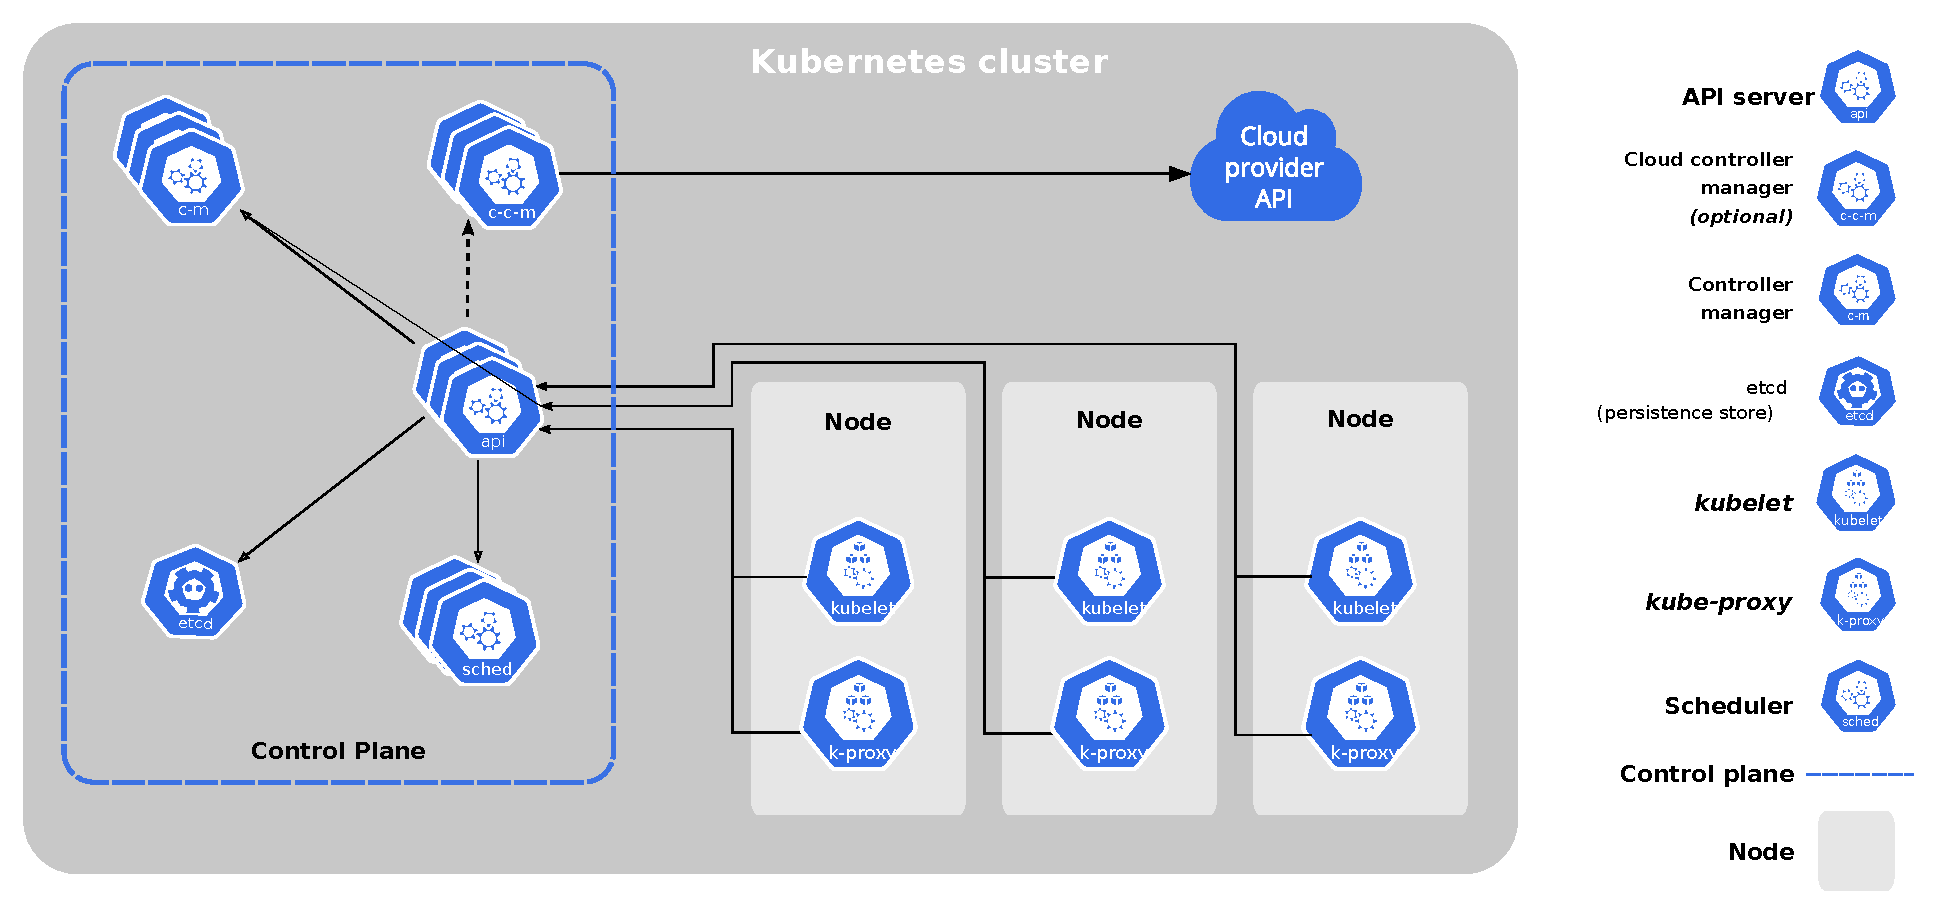
\includegraphics[width=.84\linewidth]{assets/components-of-kubernetes.pdf}
	\legend{Fonte: \citeonline{kubernetesCoreComponentes}}
\end{figure}

\newpage
\subsection{Objetos e serviços Kubernetes}
Além dos componentes do \textit{Control Plane} existem outros objetos e serviços que são fundamentais para a conteinerização, funcionamento do \textit{Kubernetes}, ou são pertinentes a este trabalho. 

\subparagraph{\textit{Pods}:} representa a menor unidade de objeto no \textit{Kubernetes}. Em resumo um \textit{pod} é uma carga de trabalho que é \DIFdelbegin \DIFdel{executado }\DIFdelend \DIFaddbegin \DIFadd{executada }\DIFaddend em \textit{nodes} do \textit{cluster} no formato de um processo.
\textit{Pod} é considerado um grupo com um ou mais contêineres, os quais compartilham \DIFdelbegin \DIFdel{recurso }\DIFdelend \DIFaddbegin \DIFadd{recursos }\DIFaddend de disco e rede\DIFdelbegin \DIFdel{, cada }\DIFdelend \DIFaddbegin \DIFadd{. 
Cada }\DIFaddend \textit{pod} contém especificação declarativa da execução dos contêineres que possui. A comunicação entre os contêineres de um mesmo \textit{pod} é feita por meio de \textit{inter-process comunication (IPC)}, como semáforos \textit{SystemV}, ou, utilizando a memória compartilhada \textit{POSIX}. Por padrão, contêineres em \textit{pods} distintos não se comunicam por meio de \textit{IPC} sem configuração personalizada. Desse modo, a comunicação entre contêineres em \textit{pods} distintos é concebida via troca de mensagem utilizando protocolo \textit{IP}.

\subparagraph{\textit{ReplicaSet}:}
Considerado um serviço responsável pelo controle de réplicas de \textit{pods} solicitado. Assim, o \textit{ReplicaSet} garante a disponibilidade de um número de \textit{pods}.

\subparagraph{\textit{Deployments}:}
fornece atualizações declarativas para \textit{pods} e \textit{replicaSets}. Ou seja, o \textit{deployment} é usado para atualização de estado de \textit{pods} e \textit{ReplicaSets}. O uso comum de \textit{deployments} em relação aos \textit{pod} é na atualização de imagem do contêiner, já para \textit{ReplicaSet} seria na atualização no número de réplicas disponíveis desejado.

\subsection{Detalhes de escalonamento}
Para realizar o escalonamento dos \textit{pods}, o \textit{kube-scheduler} executa um fluxo de operações que são separadas em duas categorias: Filtragem e Ranqueamento. Em resumo, a filtragem consiste em investigar \textit{nodes} que são capazes de executar o \textit{pod} a ser escalonado, ou seja, nessa etapa há a seleção dos \textit{nodes} do \textit{cluste} que satisfazem a solicitação de recursos do \textit{pod}. O ranqueamento, por sua vez, classifica os \textit{nodes} eleitos pela filtragem e seleciona o \textit{node} que obter a maior pontuação de acordo a solicitação de recursos do \textit{pod} \cite{Kubescheduler}.

A técnica de escalonamento utilizada pelo \textit{kube-scheduler} é denominada \textit{First-Come-First-Served} (FCFS), \DIFdelbegin \DIFdel{conhecido }\DIFdelend \DIFaddbegin \DIFadd{conhecida }\DIFaddend também como \textit{First-In-First-Out} (FIFO), que consiste em escalonar os serviços pela ordem de chegada. Alguns motivos são elencados para defender a escolha dessa técnica, por exemplo, garantia da ausência de inanição e simples implementação algorítmica. Embora exista o consenso que há espaço de melhoria, substituir essa técnica de escalonamento por um algoritmo aprimorado 
requer um estudo de caso específico bem definido \cite{CarastanSantos2019}.

\subsection{Customização do \textit{kube-scheduler}}
\label{customizacao_kube_scheduler}
De acordo com \citeonline{ibm-sched} há 4 meios de customizar o escalonador do \textit{Kubernetes}, que serão abordados nessa seção.

\subparagraph{Alteração do código fonte:}
A primeira técnica consiste em clonar o repositório do código fonte do \textit{Kubernetes}, modificar o comportamento do escalonador padrão, recompilar o projeto e executar o escalonador. Essa prática não é recomendada pois há a necessidade de alinhar o código alterado com o fluxo de execução do \textit{Kubernetes}\DIFdelbegin \DIFdel{, o }\DIFdelend \DIFaddbegin \DIFadd{.
O }\DIFaddend segundo fator que desmotiva esse método, é que o próprio \textit{Kubernetes} oferece meios para alterar o comportamento do escalonador sem a necessidade de alterar o código fonte.

\subparagraph{Múltiplos escalonadores:}
A segunda técnica é executar um escalonador customizado ao lado do escalonador padrão. O escalonador customizado é conteinerizado no formato de \textit{pod} e orquestrado pelo próprio \textit{Kubernetes}. Para que o escalonador padrão e o customizado não disputem os mesmos \textit{pods}, na criação \DIFdelbegin \DIFdel{do }\DIFdelend \DIFaddbegin \DIFadd{de novos }\DIFaddend \textit{\DIFdelbegin \DIFdel{pod}\DIFdelend \DIFaddbegin \DIFadd{pods}\DIFaddend } é preciso identificar o método de escalonamento por meio do nome do escalonador. Caso contrário, a co-existência de múltiplos escalonadores causa o bloqueio de sincronização. 
\DIFdelbegin \DIFdel{A comunicação do }\textit{\DIFdel{pod}}%DIFAUXCMD
\DIFdel{, abstraído em escalonador de contêineres, com a }\textit{\DIFdel{API}} %DIFAUXCMD
\DIFdel{do }\textit{\DIFdel{Kubernetes}} %DIFAUXCMD
\DIFdel{é custosa. Pois o }\textit{\DIFdel{pod}} %DIFAUXCMD
\DIFdel{irá consumir a }\textit{\DIFdel{API}} %DIFAUXCMD
\DIFdel{do }\textit{\DIFdel{Kubernetes}} %DIFAUXCMD
\DIFdel{por meio do protocolo }%DIFDELCMD < \ac{HTTP}%%%
\DIFdel{.
}\DIFdelend %DIF > A comunicação do \textit{pod}, abstraído em escalonador de contêineres, com a \textit{API} do \textit{Kubernetes} é custosa. Pois o \textit{pod} irá consumir a \textit{API} do \textit{Kubernetes} por meio do protocolo \ac{HTTP}.

\subparagraph{Extensão do escalonador padrão:}
A terceira solução é denominada Extensão, considerada a solução mais simples, que objetiva adicionar funcionalidades extras ao \textit{kube-scheduler}. Extensão é entendido como a configuração de ganchos (\textit{webhooks}) que o \textit{Kubernetes} oferece para executar filtragem e ranqueamento dos \textit{nodes} de forma customizada. Ganchos devem ser interpretados como gatilhos, que são funções personalizadas que o \textit{Kubernetes} engatilha para alterar algum comportamento padrão ou adicionar novas funcionalidades. Devido a simplicidade, esse método apresenta algumas limitações. 
\DIFdelbegin \DIFdel{A }\DIFdelend \DIFaddbegin \DIFadd{Por exemplo, a }\DIFaddend transferência de dados, entre o escalonador customizado e o padrão, é realizada via protocolo \ac{HTTP}, ocasionando custo alto de comunicação. O segundo problema está relacionado com a própria limitação da abordagem, pois altera apenas os procedimentos das fases de filtragem e ranqueamento, não atuando no início nem no fim de nenhuma outra etapa de escalonamento. 

\subparagraph{\textit{Framework} de escalonamento:}
O quarto método de customizar o escalonador padrão do \textit{Kubernetes} é denominado \textit{framework} de escalonamento. Essa técnica consiste em adicionar pontos de extensão no escalonador padrão do \textit{Kubernetes}, chamados \textit{plugins}, que são incluídos em tempo de compilação. Os \textit{plugins} podem ser habilitados, desabilitados e reordenados. \textit{Plugins} são adicionados nos ciclos padrões de escalonamento -- \textit{scheduling} e \textit{binding}. No ciclo \textit{scheduling} está habilitado a extensão por meio de 8 \textit{plugins}: \textit{sort, PreFilter, Filter, PreScore, Score, NormalizeScore, Reserve, Permit}. Já, na fase de \textit{binding} há 3 pontos de extensão: \textit{PreBind, Bind, PostBind}. O presente trabalho não realizará revisão completa sobre os pontos de extensão, uma vez que a documentação explora este assunto de forma ampla \cite{schedulerframework}.

\DIFaddbegin \DIFadd{\textcolor{red}{TODO: qual voce usará? Deixe claro aqui.}
}

\DIFaddend \subsection{Alta disponibilidade}
A configuração de um \textit{cluster} \textit{Kubernetes} visando alta disponibilidade é essencial para o uso de aplicações conteinerizadas em produção. A alta disponibilidade é alcançada a partir da replicação do \textit{node} \textit{master}, com isso, eliminando um único ponto de falha para os componentes do \textit{Control Plane}, que são fundamentais para o funcionamento do \textit{Kubernetes} \cite{Kubeha}.

Em uma implantação do \textit{Kubernetes} com configuração \DIFaddbegin \DIFadd{padrão }\DIFaddend de alta disponibilidade, a instância do banco de dados \textit{etcd} será \DIFdelbegin \DIFdel{replicadas }\DIFdelend \DIFaddbegin \DIFadd{replicada, }\DIFaddend utilizando um algoritmo de consenso, e todos os servidores \textit{kube-apiserver} estarão disponíveis por meio de um balanceador de carga. \DIFdelbegin \DIFdel{Enquanto que }\DIFdelend \DIFaddbegin \DIFadd{Ainda, }\DIFaddend os demais componentes (\textit{Kube-controller-manager}, \textit{Cloud-controller-manager}, \textit{kube-scheduler}) estarão apenas com uma instância ativa no \textit{cluster}. Portanto, a replicação do \textit{node master} torna-se uma solução eficaz para tolerância a falhas, contudo, não resolve a escalabilidade do problema de escalonamento. Isso ocorro porque as réplicas do \textit{kube-scheduler} não atuam em conjunto no processo de escalonamento.

\section{Microsserviços}

De acordo com \citeonline{FowlerMicrosservice} não há definição precisa de microsserviços, contudo, existem algumas características em comum acerca das implantações dessa arquitetura. Como por exemplo, um conjunto de serviços que constitui um sistema, controle descentralizado da informação, automação da implantação de \DIFdelbegin \DIFdel{software }\DIFdelend \DIFaddbegin \textit{\DIFadd{software}} \DIFaddend e uso heterogêneo de linguagens de programação e banco de dados.
\DIFaddbegin \DIFadd{Detalhes sobre definições e conceitos de microsserviços são revisados na presente seção, uma vez que o presente trabalho utilizará tal abordagem para implementação do escalonador.
}\DIFaddend 

\subsection{Definições e conceitos}
A arquitetura de microsserviços visa o desenvolvimento de um sistema como um conjunto de serviços sucintos seccionados em processos independentes, podendo ou não compartilhar o mesmo hospedeiro \cite{lewis2012microservices}. Isto é, microsserviços são pequenas aplicações que podem ser implantadas, escaladas e testadas independentemente, que possuem um conjunto limitado de funcionalidades para resolver um só objetivo. Uma única responsabilidade, por um lado, deve ser \DIFdelbegin \DIFdel{interpretado }\DIFdelend \DIFaddbegin \DIFadd{interpretada }\DIFaddend como uma única razão para mudar ou uma única razão para ser \DIFdelbegin \DIFdel{substituído}\DIFdelend \DIFaddbegin \DIFadd{substituída}\DIFaddend . Por outro lado, deve ser interpretada como um sistema que \DIFdelbegin \DIFdel{possuí }\DIFdelend \DIFaddbegin \DIFadd{possui }\DIFaddend uma funcionalidade apenas, o qual tem de ser facilmente  compreendido fora de seu contexto. Considera-se que o conceito de microsserviço está relacionado com a filosofia \textit{unix}: "Escreva programas que façam apenas uma coisa, mas que façam bem feita" e "Escreva programas que trabalhem juntos" \cite{thones2015microservices}.

\DIFdelbegin \DIFdel{Para a interação entre os serviços que compõe um sistema, os microsserviços se beneficiam de protocolos leves para troca de mensagem, como }%DIFDELCMD < \ac{RPC}%%%
\DIFdel{, protocolo de mensagens e, se for necessário, é possível utilizar }%DIFDELCMD < \ac{HTTP}%%%
\DIFdel{. O }%DIFDELCMD < \ac{HTTP} %%%
\DIFdel{é a forma habitual  que o navegador carrega páginas da }%DIFDELCMD < \ac{WWW}%%%
\DIFdel{, enquanto que, }%DIFDELCMD < \ac{RPC} %%%
\DIFdel{e fila de mensagens são protocolos comumente empregado para comunicação de sistemas distribuídos \mbox{%DIFAUXCMD
\cite{ericraymond2003}}\hspace{0pt}%DIFAUXCMD
.
}\DIFdelend %DIF > Para a interação entre os serviços que compõe um sistema, os microsserviços se beneficiam de protocolos leves para troca de mensagem, como \ac{RPC}, protocolo de mensagens e, se for necessário, é possível utilizar \ac{HTTP}~\cite{ericraymond2003}.
\DIFaddbegin 

%DIF > . O \ac{HTTP} é a forma habitual  que o navegador carrega páginas da \ac{WWW}, enquanto que, \ac{RPC} e fila de mensagens são protocolos comumente empregado para comunicação de sistemas distribuídos 
\DIFaddend 

\subsection{Do monolítico ao microsserviços}
Em engenharia de \DIFdelbegin \DIFdel{software}\DIFdelend \DIFaddbegin \textit{\DIFadd{software}}\DIFaddend , um sistema monolítico \DIFdelbegin \DIFdel{constituí-se }\DIFdelend \DIFaddbegin \DIFadd{constitui-se }\DIFaddend de uma única unidade, \DIFaddbegin \DIFadd{ou seja, }\DIFaddend todo código é vinculado a um único processo. Aplicações comerciais geralmente são dividas em três partes, lado cliente, habitualmente uma página \textit{web}, banco de dados e uma aplicação do lado servidor. Em uma aplicação \textit{web}, esse servidor lida com o \ac{HTTP}, executa a regra de domínio e persiste informações no banco de dados. O sistema do lado servidor é considerado \DIFdelbegin \DIFdel{um }\DIFdelend monolítico. Por consequência, qualquer alteração no sistema influenciará em construir e implantar uma nova versão da aplicação.

Desenvolver de forma monolítica é a maneira natural de construir sistemas, \DIFaddbegin \DIFadd{sendo que }\DIFaddend toda a lógica é gerenciada por um único processo. O projeto para esse tipo de sistema equivale a segregar as partes/módulos do sistema por meio das técnicas de programação da linguagem utilizada, por exemplo classes, interfaces, hierarquia, etc. Entretanto, sistemas monolíticos não \DIFdelbegin \DIFdel{performam na questão de escalabilidade. Pois escalar monolítico }\DIFdelend \DIFaddbegin \DIFadd{oferecem escalabilidade, pois escalar tal sistema }\DIFaddend consiste em replicar o sistema de forma integral. 
\DIFdelbegin \DIFdel{Já em }\DIFdelend \DIFaddbegin \DIFadd{Por sua vez, }\DIFaddend uma aplicação baseada em microsserviços proporciona um escalabilidade inteligente, pois replica as partes de acordo com a necessidade por meio de um balanceador de carga dedicado para cada serviço, como ilustra a \DIFdelbegin \DIFdel{figura }\DIFdelend \DIFaddbegin \DIFadd{Figura~}\DIFaddend \ref{monolitico-microsservico}.

\begin{figure}[ht!]
    \caption{\label{monolitico-microsservico}Comparação entre Monolítico e Microsserviços}
    \centering
    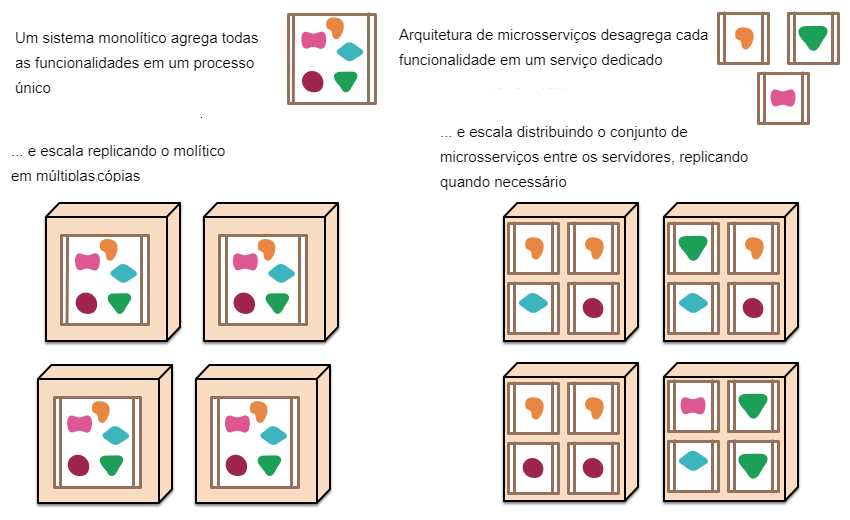
\includegraphics[width=0.85\linewidth]{assets/monilitico-microsservico.png}
    \legend{Fonte: \citeonline{FowlerMicrosservice}}
\end{figure}

\subsection{Projeto de Microsserviço guiado pelo \textit{DDD}}
O \ac{DDD}, no contexto de engenharia de \DIFdelbegin \DIFdel{software}\DIFdelend \DIFaddbegin \textit{\DIFadd{software}}\DIFaddend , é uma metodologia que conecta conceitos de linguagem de programação, por exemplo nome de classes, métodos, e atributos com o domínio do negócio \cite{DDD}. Define-se domínio como a área de conhecimento, ou seja, as funcionalidades do sistema a nível de negócio \cite{evans2014domain}.
\DIFdelbegin %DIFDELCMD < 

%DIFDELCMD < %%%
\DIFdelend %DIF > 
De acordo com \citeonline{FowlerMicrosservice}, o \ac{DDD} decompõe um domínio complexo em múltiplas partes, \DIFdelbegin \DIFdel{na literatura é definido }\DIFdelend \DIFaddbegin \DIFadd{sendo definido na literatura }\DIFaddend como contextos delimitados (\textit{bounded context}), como também visa o projeto do relacionamento entre esses. Este padrão é \DIFdelbegin \DIFdel{utilizada }\DIFdelend \DIFaddbegin \DIFadd{utilizado }\DIFaddend tanto para projetar sistemas monolíticos quanto \DIFdelbegin \DIFdel{distribuída em microsserviços. Nota-se uma correlação semântica entre um serviço e um contexto delimitado, que reforça a separação lógica do domínio em serviços isolados, consequentemente, }\DIFdelend \DIFaddbegin \DIFadd{distribuídos }\DIFaddend em microsserviços. 
\DIFdelbegin \DIFdel{Isto é, o contexto delimitado do conceito do }%DIFDELCMD < \ac{DDD} %%%
\DIFdel{se torna um excelente candidato à um microsserviço \mbox{%DIFAUXCMD
\cite{newman2015building}}\hspace{0pt}%DIFAUXCMD
. Contudo, nem todo contexto delimitado deve ser relacionado à um microsserviço independente. Segundo o criador do }%DIFDELCMD < \ac{DDD}%%%
\DIFdel{, Eric Evans, há diferentes tipos de contexto delimitado que não mapeiam diretamente a um serviço isolado.
}%DIFDELCMD < 

%DIFDELCMD < %%%
\DIFdelend %DIF > Nota-se uma correlação semântica entre um serviço e um contexto delimitado, que reforça a separação lógica do domínio em serviços isolados, consequentemente, em microsserviços. Isto é, o contexto delimitado do conceito do \ac{DDD} se torna um excelente candidato à um microsserviço \cite{newman2015building}. Contudo, nem todo contexto delimitado deve ser relacionado à um microsserviço independente. Segundo o criador do \ac{DDD}, Eric Evans, há diferentes tipos de contexto delimitado que não mapeiam diretamente a um serviço isolado.
Um dos desafios de projetar sistemas baseados em serviços distribuídos é determinar a granularidade em termos de escopo e complexidade do microsserviço. O conjunto de funções que definem o microsserviço não deve ser extremamente simplista, muito menos agregar muita complexidade \cite{merson2020modeling}. Portanto, para permitir o gerenciamento descentralizado de acordo com o contexto do domínio, o ideal é unir os princípios do \ac{DDD} com a arquitetura de microsserviços.
%DIF > 
\DIFaddbegin \DIFadd{Tal abordagem é seguida na presente proposta de escalonamento de contêineres, formalmente descrita no Capítulo~3.
}\DIFaddend 

\section{Escalonamento de \DIFdelbegin \DIFdel{Tarefas}\DIFdelend \DIFaddbegin \DIFadd{Contêineres}\DIFaddend }

\DIFdelbegin \DIFdel{Escalonamento consiste }\DIFdelend \DIFaddbegin \DIFadd{O escalonamento consiste em }\DIFaddend um processo de tomada de decisão, que é usado regularmente no ramo da manufatura, serviços industriais e sistemas operacionais. O escalonamento lida com alocação de recursos para tarefas em determinados períodos de tempo, visando otimizar um ou mais objetivos \cite{pinedo2012scheduling}. Sendo alguns desses objetivos, por exemplo, redução do tempo de espera das tarefas, maximização do uso de recursos (espalhamento), ou minimização do uso total de recursos (agrupamento).

Neste trabalho, escalonamento é um procedimento \DIFdelbegin \DIFdel{o qual soluciona }\DIFdelend \DIFaddbegin \DIFadd{que soluciona as }\DIFaddend alocações de recursos computacionais. Recursos refletem em quantidade mensurável de memória, processamento e dispositivos de rede de um \DIFdelbegin \DIFdel{, ou conjunto, de }\DIFdelend \DIFaddbegin \DIFadd{ou mais }\DIFaddend nós computacionais  (também denominado por máquinas). \DIFdelbegin \DIFdel{Segundo \mbox{%DIFAUXCMD
\citeonline{brucker1999resource}}\hspace{0pt}%DIFAUXCMD
, considere que }\DIFdelend \DIFaddbegin \DIFadd{Formalmente, segundo \mbox{%DIFAUXCMD
\citeonline{brucker1999resource}}\hspace{0pt}%DIFAUXCMD
, }\DIFaddend $m$ máquinas $M_j (j = 1, \dots, m)$ \DIFdelbegin \DIFdel{deverão }\DIFdelend \DIFaddbegin \DIFadd{devem }\DIFaddend processar $n$ trabalhos $J_i (i = 1, \dots, n)$. 
Vinculado a cada trabalho $J_i$ há um número \DIFdelbegin \DIFdel{$n_i$ de tarefas $(O_{i1}, O_{i2}, \dots, O_{in_i})$, }\DIFdelend \DIFaddbegin \DIFadd{$t_i$ de tarefas $(O_{i1}, O_{i2}, \dots, O_{it_i})$, e }\DIFaddend para cada tarefa há uma solicitação de recursos $p_{ij}$. 
Dessa forma, o escalonamento é um processo de tomada de decisão que, a partir da requisição de recursos \DIFdelbegin \DIFdel{da tarefa}\DIFdelend \DIFaddbegin \DIFadd{das tarefas}\DIFaddend ,  investigará os nós computacionais  factíveis e indicará o escalonamento ideal de $J_i$ para $M_j$ de acordo com a otimização de alguma métrica de interesse. Um escalonamento válido para alocação de trabalhos pode ser representado por meio do diagrama de Gantt, como exemplifica a \DIFdelbegin \DIFdel{figura \ref{gantt-schedulling}.
}\DIFdelend \DIFaddbegin \DIFadd{Figura \ref{gantt-schedulling}.
\textcolor{red}{TODO: explique a figura. Por qual motivo repete os índices dos jobs??? Explique o que está desenhado.}
}\DIFaddend 

\begin{figure}[ht!]
    \caption{\label{gantt-schedulling}Visualização escalonamento por meio do diagrama de Gantt}
    \centering
    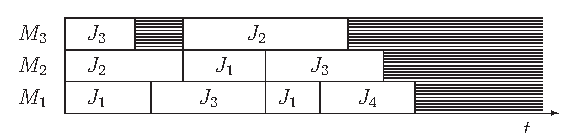
\includegraphics[width=\linewidth]{assets/gantt-scheduling.pdf}
    \legend{Fonte: \citeonline{brucker1999resource}}
\end{figure}

De acordo com \cite{pinedo2012scheduling}, o problema de escalonamento é representado por uma tripla $\alpha|\beta|\gamma$. O campo $\alpha$ representa o ambiente, interpreta-se como o perfil da arquitetura que detém os recursos em que os trabalhos serão escalonados. O campo $\beta$ define detalhes de processamento e restrições que estão vinculados ao trabalho, pode conter nenhuma, uma única ou várias entradas. Já o campo $\gamma$ descreve a função objetivo a qual visa otimização de alguma métrica de interesse, normalmente contém apenas uma entrada.

Para este trabalho, a entrada $\gamma$ será definida pelo perfil \textbf{Máquinas em Paralelo com Diferentes Velocidades} e é representado pelo rótulo $Qm$. Este cenário consiste em $m$ máquinas heterogêneas, que não necessariamente possuem a mesma quantidade de recursos. Considera-se a principal abordagem das nuvens computacionais atualmente \cite{krauter2002taxonomy}.

A entrada $\beta$ é definida pelo conjunto \textbf{Prazo ou \textit{deadline}} ($P$), \textbf{Restrição de Elegibilidade} ($M$) e \textbf{Processamento em Lote} ($batch(b)$). Se o rótulo $P$ está presente em $\beta$, então para cada trabalho $J_{k}$ será atribuído um prazo de entrega $P_{k}$, dessa forma, $J_k$ não deve ser escalonado após o prazo $P_{k}$. Se $P$ não está incluído em $\beta$, logo não há restrição de \textit{deadline} de escalonamento. O rótulo $M$ denota que nem todas as máquinas são capazes de processar o trabalho $J_{k}$, assim, o conjunto $M_{k}$ representa as máquinas que satisfazem as restrições de $J_{k}$, que por consequência, são elegíveis ao escalonamento. Por último, se há rótulo $batch(b)$ em $\beta$, então, uma máquina é apta a processar quantidade $b$ de trabalhos de forma simultânea.

Portanto, $\beta=\{P, M, batch(b)\}$. O campo $\gamma$, que está relacionado com métricas de escalonamento e funções objetivos, será desenvolvido na seção subsequente.

\subsection{Métricas de Escalonamento e Função Objetivo}
De acordo com \cite{Feitelson98}, há um conjunto de métricas relevantes a respeito do desempenho de algoritmos de escalonamentos. O presente trabalho visa a otimização das seguintes métricas: tempo de espera de escalonamento \DIFdelbegin \DIFdel{, }\DIFdelend \DIFaddbegin \DIFadd{e }\DIFaddend \textit{makespan}. Além disso, \DIFaddbegin \DIFadd{ocorrerá a }\DIFaddend análise do comportamento do \textit{slowdown}.

\subsubsection{Tempo de Espera}
\DIFdelbegin \DIFdel{Considere }\DIFdelend \DIFaddbegin \DIFadd{Considerando }\DIFaddend $Submetido_k$ \DIFaddbegin \DIFadd{como }\DIFaddend o momento em que o trabalho $J_k$ foi submetido à plataforma, $Inicio_k$ o momento em que o trabalho $J_k$ iniciou sua execução\DIFdelbegin \DIFdel{. A }\DIFdelend \DIFaddbegin \DIFadd{, a }\DIFaddend Equação \ref{eq:1} mensura o tempo de espera, ou seja, o tempo que o trabalho permanece na fila até ser escalonado.
\DIFdelbegin \DIFdel{Para um trabalho $J_k$ o tempo de espera $T_k$ é determinado pela equação:
}\DIFdelend 

\begin{equation} \label{eq:1}
T_k = Inicio_k - Submetido_k
\end{equation}

\DIFdelbegin \DIFdel{Minimização }\DIFdelend \DIFaddbegin \DIFadd{A minimização }\DIFaddend do tempo de espera é um \DIFdelbegin \DIFdel{problema de escalonamento conhecido }\DIFdelend \DIFaddbegin \DIFadd{objetivo conhecido e }\DIFaddend importante no fornecimento de \textit{Quality of Service (QoS)} em \DIFdelbegin \DIFdel{muitas indústrias }\DIFdelend \DIFaddbegin \DIFadd{muitos cenários }\DIFaddend \cite{Ye2007}. Por ser classificado como um problema \textit{NP-Hard} \cite{Kubiak1993}, na literatura \DIFdelbegin \DIFdel{é encontrada }\DIFdelend \DIFaddbegin \DIFadd{são encontradas }\DIFaddend diferentes heurísticas que aproximam-se da solução ideal, pois não há algoritmo de busca eficiente que encontre uma sequência ótima\DIFdelbegin \DIFdel{\mbox{%DIFAUXCMD
\cite{Ye2007}}\hspace{0pt}%DIFAUXCMD
}\DIFdelend .

\subsubsection{\textit{Makespan}}
A próxima métrica a ser considerada é o \textit{makespan}, que é uma métrica diretamente vinculada ao tempo de completude de um trabalho. O cálculo é definido pelo tempo de término da última tarefa de um trabalho a deixar o sistema. \DIFdelbegin \DIFdel{Considere }\DIFdelend \DIFaddbegin \DIFadd{Considerando }\DIFaddend que um trabalho $J_k$ possui $n$ tarefas vinculadas $O_{k,1}, O_{k,2}, ..., O_{k,n}$, e para cada tarefa $O_{k,i}$ há vinculado \DIFaddbegin \DIFadd{o }\DIFaddend tempo de finalização $C_i$, assim o \textit{makespan} $C_{max, k}$ de $J_k$ é calculado de acordo com a \DIFdelbegin \DIFdel{equação:
}\DIFdelend \DIFaddbegin \DIFadd{Equação~\ref{eq:make}.
}\DIFaddend 

\begin{equation} \DIFaddbegin \label{eq:make}
\DIFaddend C_{max,k} = max(C_1, C_2, ..., C_n) 
\end{equation}

A minimização do \textit{makespan} resulta na otimização da utilização dos recursos computacionais \cite{pinedo2012scheduling}\DIFdelbegin \DIFdel{. Pois }\DIFdelend \DIFaddbegin \DIFadd{, pois }\DIFaddend o \textit{makespan} está relacionado ao tempo que o trabalho permanece na plataforma\DIFaddbegin \DIFadd{.
Ainda}\DIFaddend , a sua minimização acarreta em melhor agrupamento do escalonamento, que por consequência, ocorrendo a liberação do uso de recursos em um menor período de tempo.

\subsubsection{\textit{Slowdown}}
Por último, outra métrica abordada neste trabalho é o \textit{slowdown}, que é definido pela relação entre o tempo total que o trabalho permaneceu na plataforma com o tempo atual de processamento gasto com o mesmo. Assim o \textit{slowdown} $Sd_k$ de $J_k$  é definido pela Equação \ref{eq:2}\DIFdelbegin \DIFdel{:
}%DIFDELCMD < 

%DIFDELCMD < %%%
\begin{displaymath} \DIFdel{%DIFDELCMD < \label{eq:2}%%%
Sd_{k} = \frac{T_{k} + P_{k}}{P_{k}}
}\end{displaymath}%DIFAUXCMD
%DIFDELCMD < 

%DIFDELCMD < %%%
\DIFdelend \DIFaddbegin \DIFadd{, sendo que }\DIFaddend \(P_{k}\) é o tempo de processamento de \(J_k\).
\DIFaddbegin 

\begin{equation} \DIFadd{\label{eq:2}
Sd_{k} = \frac{T_{k} + P_{k}}{P_{k}}
}\end{equation}

\DIFaddend O propósito do \textit{slowdown} é estabelecer  proporção entre tempo de espera de um trabalho em relação ao seu tempo de processamento \cite{Maccio2018}, com o objetivo de atribuir uma distribuição equilibrada do tempo de espera entre os trabalhos com diferentes cargas de trabalho \cite{CarastanSantos2019}.

\subsubsection{Função Objetivo}
Portanto o campo $\gamma$ (função objetivo) da definição de escalonamento refere-se à minimização do tempo de espera, \textit{makespan}, logo, $\gamma = T, C_{max}$. Em cenários como \ac{HPC}, os resultados visados por meio da otimização desse conjunto de métricas são: Melhor \textit{QoS} por meio da minimização do tempo de espera; Otimizar a utilização dos recursos computacionais mediante a minimização do \textit{makespan}; \DIFaddbegin \DIFadd{e }\DIFaddend Analisar o comportamento do \textit{slowdown}.

\subsection{Escalonamento Distribuído}

Aplicações atuais fundamentam-se na análise e processamento de um grande volume de dados, como por exemplo, \textit{Data Mining}, \textit{Machine Learning}, \textit{Deep Learning} e banco de dados. Dessa forma, conforme a demanda de poder computacional cresce, as estruturas responsáveis pela execução dessas aplicações os acompanham, refletindo no aumento de complexidade tanto em tamanho como em algoritmos refinados de gerenciamento \cite{Wang2016LoadbalancedAL}. A nível de comparação desse reflexo, a empresa \textit{Google} executa centenas de milhares de cargas de trabalho, de \DIFdelbegin \DIFdel{muitos }\DIFdelend milhares de aplicativos em \DIFdelbegin \DIFdel{uma }\DIFdelend \DIFaddbegin \DIFadd{um }\DIFaddend conjunto de \textit{clusters}, cada qual com até dezenas de milhares de máquinas \cite{Google2015Borg}. 
Por consequência, os componentes \DIFdelbegin \DIFdel{internos }\DIFdelend de gerenciamento de um \textit{data center} de larga escala \DIFdelbegin \DIFdel{deve }\DIFdelend \DIFaddbegin \DIFadd{devem }\DIFaddend resolver os problemas internos com algoritmos complexos e sofisticados para cada tipo de cenário.

O escalonamento é um tema amplamente pesquisado, desde \DIFdelbegin \DIFdel{de }\DIFdelend otimização por meio de processamento em \textit{GPU} \cite{Nesi2018ScheduleGPU} como também baseado em arquitetura descentralizada empregando conceitos de \textit{blockchain} \cite{loch2021novel}. De acordo com a literatura, \DIFaddbegin \DIFadd{o }\DIFaddend escalonamento distribuído \DIFdelbegin \DIFdel{, hoje, }\DIFdelend é requisito fundamental para \textit{Data Centers} de larga escala \cite{Google2015Borg, Wang2019Pigeon}\DIFdelbegin \DIFdel{. Uma vez que , }\DIFdelend \DIFaddbegin \DIFadd{, uma vez que }\DIFaddend a principal dificuldade da abordagem centralizada está na escalabilidade e nos métodos de tolerâncias a falhas, que degradam por completo as métricas de \ac{QOS}. O escalonamento, no formato distribuído, resolve este problema de forma elaborada removendo o único ponto de falha ao particionar as requisições de alocação de recursos em um sistema distribuído.

\section{Trabalhos Relacionados}

A área de escalonamento de tarefas \DIFdelbegin \DIFdel{é estudada a décadas, considera-se um ramo com }\DIFdelend \DIFaddbegin \DIFadd{realiza a }\DIFaddend intersecção \DIFdelbegin \DIFdel{em }\DIFdelend \DIFaddbegin \DIFadd{de }\DIFaddend diferentes campos da ciência da computação. Um dos principais fatores que impulsionam a intersecção entre as áreas está na natureza do problema de escalonamento, pois \DIFdelbegin \DIFdel{na maioria dos casos }\DIFdelend resolver um problema de escalonamento reflete em otimizar um problema \textit{NP-difícil}. Dessa forma, na literatura \DIFdelbegin \DIFdel{, encontra-se }\DIFdelend \DIFaddbegin \DIFadd{encontram-se }\DIFaddend diferentes pesquisas que refletem em soluções heurísticas e refinadas, muitas vezes relacionadas com a área de inteligência artificial. Por se tratar da solução de um problema \textit{\DIFdelbegin \DIFdel{np-difícil}\DIFdelend \DIFaddbegin \DIFadd{Np-difícil}\DIFaddend }, a solução computada basta ser boa o suficiente para um cenário específico, sendo assim, a solução encontrada nem sempre é refletida na ótima global.

Esta seção analisará trabalhos recentes da literatura que possuem relação com escalonamento de contêineres. Por ainda se tratar de um recorte amplo na área de escalonamento, aqui \DIFdelbegin \DIFdel{analisou-se }\DIFdelend \DIFaddbegin \DIFadd{analisaram-se }\DIFaddend diferentes trabalhos que atacam \DIFdelbegin \DIFdel{diferentes }\DIFdelend características \DIFdelbegin \DIFdel{, seja relacionado }\DIFdelend \DIFaddbegin \DIFadd{distintas, sejam relacionadas }\DIFaddend com otimização energética em \textit{data centers} como também trabalhos que buscaram otimizar o desempenho de escalonamento.

\DIFdelbegin \subsection{\DIFdel{Redução do custo energético}}
%DIFAUXCMD
\addtocounter{subsection}{-1}%DIFAUXCMD
\DIFdelend No trabalho de \citeonline{sureshkumar2017optimizing} os autores propuseram um algoritmo de escalonamento de contêineres, para a tecnologia \textit{docker}, baseado em balanceamento de carga. O algoritmo consiste em um limiar calculado a partir da sobrecarga do \textit{cluster}\DIFdelbegin \DIFdel{, o }\DIFdelend \DIFaddbegin \DIFadd{.
O }\DIFaddend objetivo do limiar é que as cargas dos contêineres não sejam \DIFdelbegin \DIFdel{muito altas e }\DIFdelend \DIFaddbegin \DIFadd{altas ou }\DIFaddend baixas. Quando a carga ultrapassa o limiar, um novo contêiner é criado no balanceamento de carga. Por outro lado, quando a carga é muito baixa, o contêiner é destruído com o objetivo de economizar custo energético.

\DIFdelbegin \subsection{\DIFdel{Otimização multi objetivo}}
%DIFAUXCMD
\addtocounter{subsection}{-1}%DIFAUXCMD
\DIFdel{Em }\DIFdelend \DIFaddbegin \DIFadd{Por sua vez, em }\DIFaddend \citeonline{liu2018new} os autores desenvolveram um novo algoritmo de escalonamento de contêineres denominado \textit{multipot}. Neste projeto \DIFdelbegin \DIFdel{foi estudado }\DIFdelend \DIFaddbegin \DIFadd{foram estudados }\DIFaddend múltiplos critérios para a seleção de um \textit{node} para provisionar o contêiner. O algoritmo considera cinco métricas chaves: \DIFdelbegin %DIFDELCMD < \begin{enumerate}
%DIFDELCMD < 	\item %%%
\DIFdelend Uso de CPU de cada \textit{node}; \DIFdelbegin %DIFDELCMD < \item %%%
\DIFdelend Uso de memória de cada \textit{node}; \DIFdelbegin %DIFDELCMD < \item %%%
\DIFdelend Tempo da transmissão da imagem do contêiner na internet; \DIFdelbegin %DIFDELCMD < \item %%%
\DIFdelend Associação entre os contêineres e os \textit{nodes}; \DIFdelbegin %DIFDELCMD < \item %%%
\DIFdelend \DIFaddbegin \DIFadd{e }\DIFaddend Agrupamento de contêineres.
\DIFdelbegin %DIFDELCMD < \end{enumerate}
%DIFDELCMD < %%%
\DIFdelend %DIF > 
Todas essas métricas foram consideradas, pois \DIFdelbegin \DIFdel{, }\DIFdelend de acordo com os autores, afetam \DIFdelbegin \DIFdel{no }\DIFdelend \DIFaddbegin \DIFadd{o }\DIFaddend desempenho das aplicações que estão sendo executadas pelos contêineres. A função objetivo de escalonamento é a otimização da composição de todas as métricas chaves, ou seja, para cada métrica chave é relacionado um escore, \DIFdelbegin \DIFdel{esses escores }\DIFdelend \DIFaddbegin \DIFadd{que }\DIFaddend são agrupados em uma função de composição que representa a função objetivo.

Em \citeonline{menouer2019new} foi desenvolvido uma nova estratégia de escalonamento baseado em um algoritmo de decisão multi-critério. A abordagem consiste em escalonar contêineres baseado em três critérios que estão relacionados a todos os \textit{nodes}  que constitui a infraestrutura de nuvem: (1) O número de contêineres em execução; (2) A disponibilidade de CPU; (3) A disponibilidade do espaço de memória.
\DIFdelbegin %DIFDELCMD < 

%DIFDELCMD < %%%
\DIFdel{Em }\DIFdelend \DIFaddbegin \DIFadd{De forma complementar, em~}\DIFaddend \citeonline{menouer2019power} os autores utilizaram técnicas refinadas de \textit{machine learning} em um ambiente de nuvem para construção de um escalonador de contêineres. O objetivo dessa abordagem é reduzir o consumo energético de infraestruturas de nuvens heterogêneas. O \DIFdelbegin \DIFdel{principio }\DIFdelend \DIFaddbegin \DIFadd{princípio }\DIFaddend corresponde a dois passos denominados (1) aprender e (2) escalonar, que são aplicados a cada novo contêiner que é submetido à plataforma. No passo (1) é estimado o consumo energético de cada \textit{node}, logo, é elencado grupos de \textit{nodes} que formam uma estrutura de nuvem heterogênea em um \textit{cluster} de acordo com o seu consumo energético.
Já no passo (2), é selecionado o \textit{node} que corresponde  ao menor consumo energético. O algoritmo foi implementado para a plataforma \textit{docker swarm}.

\DIFdelbegin \subsection{\DIFdel{Considerações parciais}}
%DIFAUXCMD
\addtocounter{subsection}{-1}%DIFAUXCMD
\DIFdelend \DIFaddbegin \section{\DIFadd{Considerações parciais}}

\DIFadd{\textcolor{red}{TODO: aqui você precisa escrever as consideracoes do capitulo. Conecte todos os itens. Ligue os pontos. Deixe claro o que vem no próximo capítulo.}
}

\DIFaddend Está seção elencou alguns do trabalhos encontrados na literatura acerca do tema escalonamento de contêineres. Nota-se que os trabalhos envolvidos possuem definição de parâmetros e métricas de otimização, como por exemplo: consumo energético, desempenho. Por se tratar de um recorte grande na literatura, o tema escalonamento abre espaço para implementação de diferentes soluções para o problema. Todavia, os trabalhos relacionados aqui elencados não consideram o fator escalabilidade, não há nenhuma solução distribuída. A escassez de projetos de escalonamento de contêineres que envolvam o desenvolvimento de uma arquitetura distribuída, é uma das principais motivações para o presente trabalho.

% ----------------------------------------------------------

% ----------------------------------------------------------
% Trabalhos relacionados
% ----------------------------------------------------------
% \chapter{Trabalhos Relacionados}
%%
%%\textcolor{red}{Linha escalonadores distribuidos: revisao do Wilton}
%%
%%MapReduce, Spark, XYZ
%%Conclusão: a minha ideia é que pode ser usado qualquer escalonador, desde que seja possível representar como microsserviço (stateless).
%%
%%\textcolor{red}{Tecer comentários sobre TF: replicas ja foram usadas para contornar falhas. %%\url{https://gkoslovski.github.io/files/ijguc-2019.pdf}}
%%
%%Tabela de conclusao. Colunas: 1 ref, 2 foco, 3 container/VM/tarefa. Mostrar que microsservico é uma opção viavel.
%%
%%A área de escalonamento possui diversas referencias fortes em diversas áreas. Entretanto, a conteinerização é um termo recente comparado a toda história 

A área de escalonamento de tarefas é estudada a décadas, considera-se um ramo com intersecção em diferentes campos da ciência da computação. Um dos principais fatores que impulsionam a intersecção entre as áreas está na natureza do problema de escalonamento, pois na maioria dos casos resolver um problema de escalonamento reflete em otimizar um problema \textit{NP-difícil}. Dessa forma, na literatura, encontra-se diferentes pesquisas que refletem em soluções heurísticas e refinadas, muitas vezes relacionadas com a área de inteligência artificial. Por se tratar da solução de um problema \textit{np-difícil}, a solução computada basta ser boa o suficiente para um cenário específico, sendo assim, a solução encontrada nem sempre é refletida na ótima global.

Esta seção analisará trabalhos recentes da literatura que possuem relação com escalonamento de contêineres. Por ainda se tratar de um recorte amplo na área de escalonamento, aqui analisou-se diferentes trabalhos que atacam diferentes características, seja relacionado com otimização energética em \textit{data centers} como também trabalhos que buscaram otimizar o desempenho de escalonamento.

\section{Redução do custo energético}
No trabalho de \citeonline{sureshkumar2017optimizing} os autores propuseram um algoritmo de escalonamento de contêineres, para a tecnologia \textit{docker}, baseado em balanceamento de carga. O algoritmo consiste em um limiar calculado a partir da sobrecarga do \textit{cluster}, o objetivo do limiar é que as cargas dos contêineres não sejam muito altas e baixas. Quando a carga ultrapassa o limiar, um novo contêiner é criado no balanceamento de carga. Por outro lado, quando a carga é muito baixa, o contêiner é destruído com o objetivo de economizar custo energético.

\section{Otimização multi objetivo}
Em \citeonline{liu2018new} os autores desenvolveram um novo algoritmo de escalonamento de contêineres denominado \textit{multipot}. Neste projeto foi estudado múltiplos critérios para a seleção de um \textit{node} para provisionar o contêiner. O algoritmo considera cinco métricas chaves:
\begin{enumerate}
	\item Uso de CPU de cada \textit{node};
	\item Uso de memória de cada \textit{node};
	\item Tempo da transmissão da imagem do contêiner na internet;
	\item Associação entre os contêineres e os \textit{nodes};
	\item Agrupamento de contêineres.
\end{enumerate}
Todas essas métricas foram consideradas, pois, de acordo com os autores, afetam no desempenho das aplicações que estão sendo executadas pelos contêineres. A função objetivo de escalonamento é a otimização da composição de todas as métricas chaves, ou seja, para cada métrica chave é relacionado um escore, esses escores são agrupados em uma função de composição que representa a função objetivo.

Em \citeonline{menouer2019new} foi desenvolvido uma nova estratégia de escalonamento baseado em um algoritmo de decisão multi-critério. A abordagem consiste em escalonar contêineres baseado em três critérios que estão relacionados a todos os \textit{nodes}  que constitui a infraestrutura de nuvem: (1) O número de contêineres em execução; (2) A disponibilidade de CPU; (3) A disponibilidade do espaço de memória.

Em \citeonline{menouer2019power} os autores utilizaram técnicas refinadas de \textit{machine learning} em um ambiente de nuvem para construção de um escalonador de contêineres. O objetivo dessa abordagem é reduzir o consumo energético de infraestruturas de nuvens heterogêneas. O principio corresponde a dois passos denominados (1) aprender e (2) escalonar, que são aplicados a cada novo contêiner que é submetido à plataforma. No passo (1) é estimado o consumo energético de cada \textit{node}, logo, é elencado grupos de \textit{nodes} que formam uma estrutura de nuvem heterogênea em um \textit{cluster} de acordo com o seu consumo energético.
Já no passo (2), é selecionado o \textit{node} que corresponde  ao menor consumo energético. O algoritmo foi implementado para a plataforma \textit{docker swarm}.

\section{Considerações parciais}
Está seção elencou alguns do trabalhos encontrados na literatura acerca do tema escalonamento de contêineres. Nota-se que os trabalhos envolvidos possuem definição de parâmetros e métricas de otimização, como por exemplo: consumo energético, desempenho. Por se tratar de um recorte grande na literatura, o tema escalonamento abre espaço para implementação de diferentes soluções para o problema. Todavia, os trabalhos relacionados aqui elencados não consideram o fator escalabilidade, não há nenhuma solução distribuída. A escassez de projetos de escalonamento de contêineres que envolvam o desenvolvimento de uma arquitetura distribuída, é uma das principais motivações para o presente trabalho.
 


% ----------------------------------------------------------

% ----------------------------------------------------------
% Proposta
% ----------------------------------------------------------
\chapter{KMS - \textit{Kubernetes Micro Scheduler}}

Este capítulo tem como objetivo apresentar os processos de desenvolvimento do escalonador distribuído proposto, denominado \ac{KMS}. A escolha do nome está concentrada na etimologia da palavra \textbf{micro}, a qual significa \textbf{pequeno}, visto que um dos principais objetivos do presente trabalho é distribuir o escalonador utilizando conceitos de \textbf{micro}sserviços. Ou seja, fragmentar um escalonador monolítico em pequenos sistemas que operam de forma independentes, mas em conjunto refletem um sistema distribuído robusto.

No início do capítulo é apresentado um comparativo entre o \ac{KMS} com as atuais abordagens de escalonamento do \textit{Kubernetes}, o principal objetivo nesta seção é confrontar as arquiteturas em cenários de falhas. Ao passo que, as seções subsequentes são dedicadas ao funcionamento dos componentes do \ac{KMS}, como também as trocas de mensagens. Exceto a Seção 3.2, que é destinada à apresentar a documentação baseada na engenharia de requisitos para delimitar o escopo do projeto.

%O presente trabalho visa o desenvolvimento de um escalonador distribuído, baseado em microsserviços, e a sua implantação no \textit{Kubernetes}. Dessa forma, os principais objetivos do escalonador proposto são ampliar a escalabilidade visando otimizar as métricas de tempo de espera de escalonamento e \textit{makespan}, como também tratar as falhas de forma competente.

%O desafio inicial é a identificação dos microsserviços a partir de uma abordagem fundamentada em sistemas distribuídos. O segundo desafio é relacionado ao desenvolvimento do projeto, o qual será visado um sistema documentado, consistente e tolerante a falhas, alcançados por meio de uma arquitetura robusta e replicável. O terceiro desafio compreende na implantação da solução para o \textit{Kubernetes}, como também os resultados a partir das métricas de interesse.
\DIFdelbegin %DIFDELCMD < \newpage
%DIFDELCMD < %%%
\DIFdelend \DIFaddbegin 

\DIFaddend \section{Comparativo com abordagem padrão do \textit{Kubernetes}}
A visualização \DIFdelbegin \DIFdel{do desempenho }\DIFdelend \DIFaddbegin \DIFadd{da proposta e desempenho esperado }\DIFaddend do escalonador proposto \DIFdelbegin \DIFdel{distribuído }\DIFdelend é notável ao ser comparado com as demais abordagens de escalonamento que o \textit{Kubernetes} oferece (com e sem réplica do \textit{node master)}, como esboça a Figura \ref{fig:comp_sched}.
\DIFdelbegin %DIFDELCMD < 

%DIFDELCMD < \begin{figure}[h!]
%DIFDELCMD < 	%%%
%DIFDELCMD < \caption{%
{%DIFAUXCMD
%DIFDELCMD < \label{fig:comp_sched}%%%
\DIFdelFL{Comparação das abordagens de escalonamento}}
	%DIFAUXCMD
%DIFDELCMD < \centering
%DIFDELCMD < 	%%%
%DIF <  \includegraphics[width=\linewidth]{figuras/schedule-proposal.png}
	%DIF <  \hspace*{-.85in}
	%DIFDELCMD < 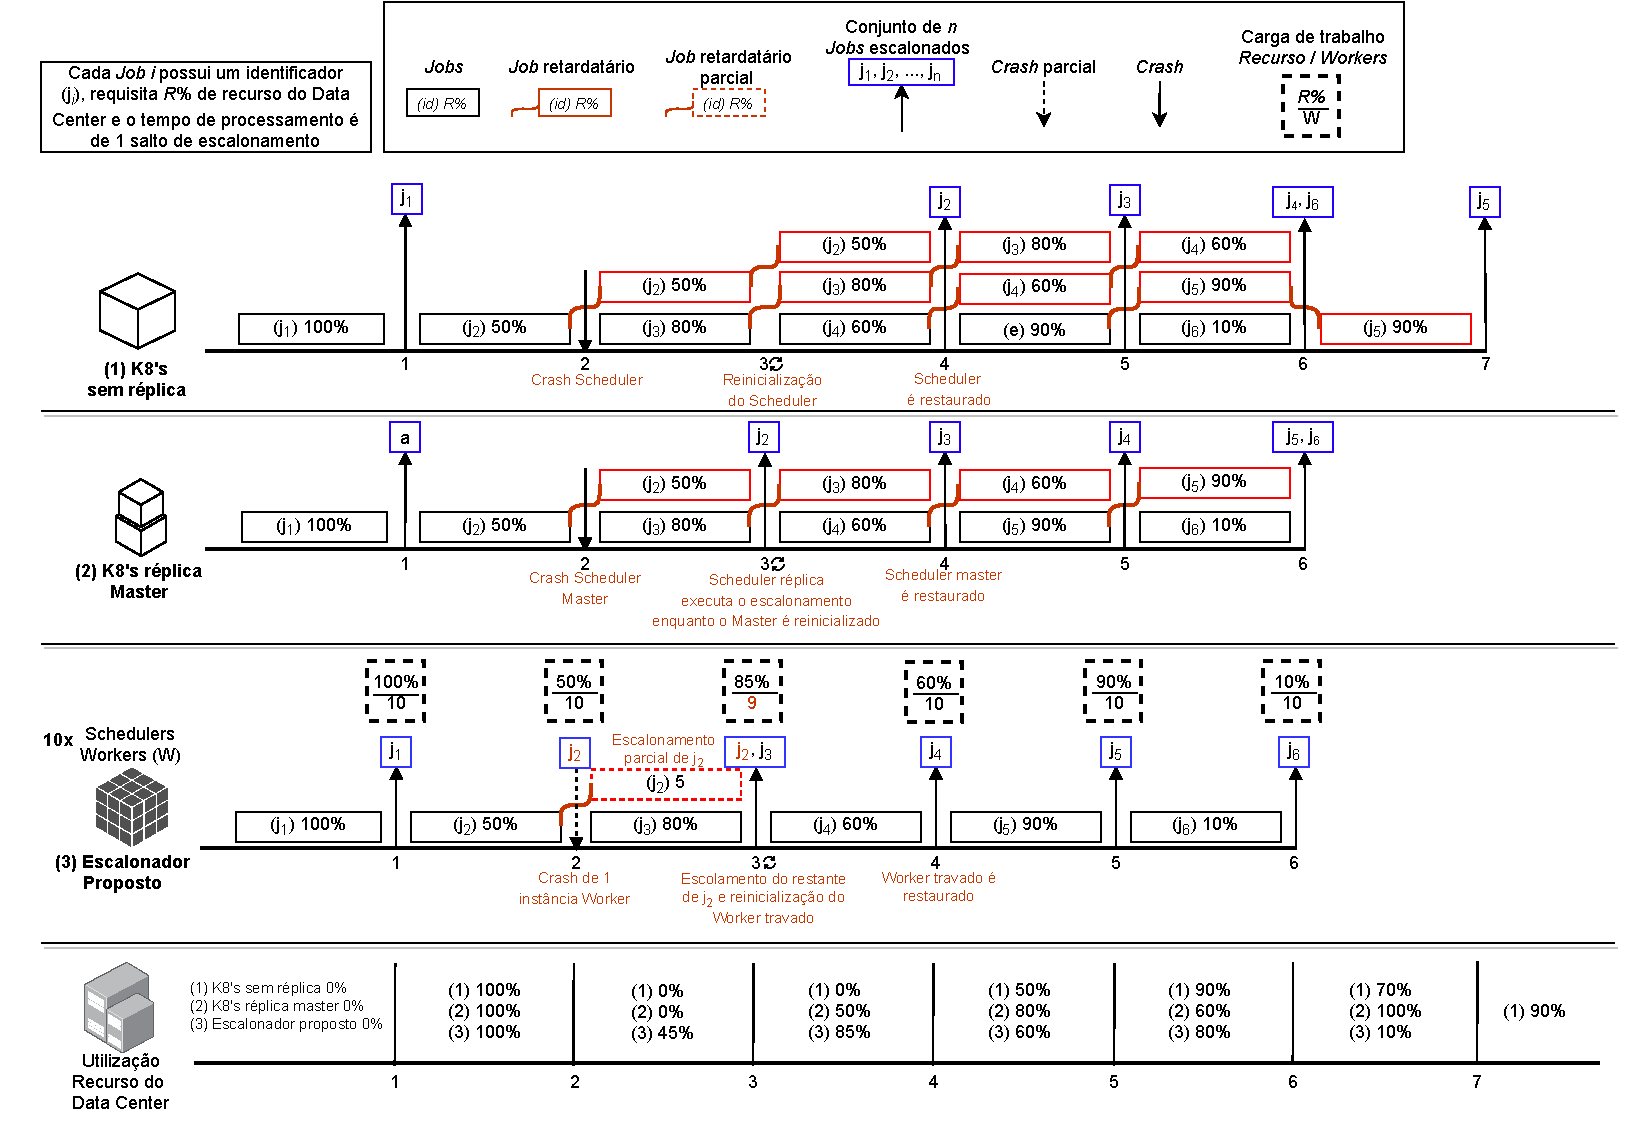
\includegraphics[width=1\linewidth]{assets/schedule-proposal.drawio.pdf}
%DIFDELCMD < 	\legend{Fonte: O autor}
%DIFDELCMD < \end{figure}
%DIFDELCMD < 

%DIFDELCMD < %%%
\DIFdel{A Figura \ref{fig:comp_sched} }\DIFdelend \DIFaddbegin \DIFadd{A figura }\DIFaddend representa o comportamento de três métodos de escalonamento de contêineres: Escalonador padrão \textit{Kubernetes} com \textit{(1)} e sem \textit{(2)} réplica e o escalonador distribuído proposto \textit{(3)} em um período de tempo dividido em eventos de escalonamento. No primeiro evento de escalonamento há uma solicitação de 100\% de uso dos recursos, e em todas as abordagens o escalonamento é executado com sucesso, pois os recursos estavam disponíveis e não ocorreram falhas.
\DIFaddbegin 

\DIFaddend No segundo evento há uma nova solicitação que consome 50\% dos recursos, entretanto, houve a simulação de uma falha do tipo \textit{crash}. Por conta disso, a abordagem \textit{(1)} utilizará um evento de escalonamento para reinicialização do sistema e a abordagem \textit{(2)} redirecionará as requisições para a réplica de escalonamento. Diferente disso, o escalonador distribuído \textit{(3)} é capaz de executar o escalonamento parcial, dado que a falha ocorreu em apenas uma unidade do sistema distribuído. A principal consequência no comportamento do escalonador \textit{(1)} e \textit{(2)} é no atraso das requisições em efeito cascata. Por consequência, todas as requisições que excedem a capacidade de recursos são atrasadas para o próximo passo de escalonamento, causando degradamento do tempo de espera e \textit{slowdown}.

%\DIFaddbegin \begin{figure}[h!]
%	\caption{\label{fig:comp_sched}\DIFaddFL{Comparação das abordagens de escalonamento}}
%	\centering
	%DIF >  \includegraphics[width=\linewidth]{figuras/schedule-proposal.png}
	%DIF >  \hspace*{-.85in}
%	\includegraphics[width=1\linewidth]{assets/schedule-proposal.pdf}
%	\legend{Fonte: O autor}
%\end{figure}

\DIFaddend \section{Levantamento de Requisitos}

Nessa seção objetiva-se desenvolver uma documentação compreensível do sistema distribuído proposto guiado pela engenharia de requisitos. O levantamento de requisitos é o passo inicial para entendimento do escopo e objetivos do \ac{KMS}, foi desenvolvido utilizando a técnica de análise de cenário e objetivos desejados. No contexto do presente trabalho, buscou-se elencar os requisitos funcionais a partir do comportamento do sistema distribuído e suas funcionalidades, já os requisitos não funcionais aqueles que representam as propriedades e restrições desejadas. 

\subparagraph{Requisitos funcionais}
\begin{enumerate}
	\item Escalonar cargas de trabalho utilizando arquitetura hierárquica de sistemas distribuídos, denominada \textit{master/\DIFdelbegin \DIFdel{slave}\DIFdelend \DIFaddbegin \DIFadd{worker}\DIFaddend };
	\item Segmentar o \textit{cluster}\DIFdelbegin \DIFdel{, cada }\DIFdelend \DIFaddbegin \DIFadd{. Cada }\DIFaddend segmento será gerenciado por um escalonador dedicado denominado \textit{worker};
	\item \textit{Workers} serão responsáveis por escalonar cargas de trabalhos nos segmentos do \textit{cluster};
	\item Implementação de estratégias de escalonamento conhecidas na literatura, como por exemplo: \textit{Round-Robin}, \textit{Binpack} e \textit{Easy Backfiling}; e
	\item Possibilidade de intercambiar o algoritmo de escalonamento.
\end{enumerate}

\subparagraph{Requisitos não funcionais}
\begin{enumerate}
	\item O escalonador deverá ser compatível com o \textit{Kubernetes};
	\item Executar os microsserviços virtualizados em contêineres;
	\item O sistema não deve conter único ponto de falha, todos os componentes deverão serem distribuídos;
	\item Desenvolver os principais componentes (\textit{Master} e \textit{Worker}) no formato de microsserviços \textit{stateless}.
	\item Desenvolver um sistema distribuído de forma transparente, ou seja, promover acesso aos recursos distribuídos de forma oculta, como se fosse um único sistema para o usuário; e
	\item Utilizar a estratégia de múltiplos escalonadores, como discutido na seção 2.2.4.
\end{enumerate}

\section{Identificação dos Componentes}

Em síntese, o \ac{KMS} consiste em um modelo hierárquico de sistema distribuído, \DIFdelbegin \DIFdel{possuí }\DIFdelend \DIFaddbegin \DIFadd{possuindo }\DIFaddend 2 componentes principais: \textit{Master} e \textit{Worker}. O componente \textit{Master} corresponde ao único ponto de centralização, isso não significa que haverá um único ponto de falha no sistema, mas sim que este componente manterá apenas uma instância ativa executando o trabalho dentre todas as suas réplicas. Ao fazer uma analogia com a arquitetura Produtor/Consumidor, o componente \textit{Worker} corresponde ao Consumidor, pois é responsável por executar as ações de escalonamento do \ac{KMS}, enquanto que o \textit{Master} é interpretado como Produtor, em razão de lidar com a delegação de trabalho.


% Baseado em um modelo hierárquico, o sistema distribuído proposto consiste em dois componentes principais: \textit{master} e \textit{worker}. O componente \textit{master} corresponde ao único ponto de centralização, já o \textit{worker} é \textit{stateless} e replicável. Cada componente possui uma responsabilidade distinta e específica e em conjunto eles representam o \ac{KMS}.

\subsection{\textit{Master}}

Responsável por buscar cargas de trabalho (\textit{pods}) na fila de escalonamento do \textit{Kubernetes}, \DIFaddbegin \DIFadd{e }\DIFaddend em seguida distribuir as cargas para os \textit{Workers}.  Ou seja, é um componente relacionado com a delegação de trabalho, considerado o \DIFdelbegin \textbf{\DIFdel{Produtor}} %DIFAUXCMD
\DIFdelend \DIFaddbegin \DIFadd{produtor }\DIFaddend em um sistema distribuído.
\DIFdelbegin %DIFDELCMD < 

%DIFDELCMD < %%%
\DIFdelend %DIF > 
Um dos princípios do desenvolvimento, não só do componente \textit{Master}, mas sim de todo o sistema, é implementar uma arquitetura modular a qual seja possível intercambiar entre as técnicas de escalonamentos \DIFaddbegin \DIFadd{(seguindo os princípios DDD previamente descritos)}\DIFaddend . 
O primeiro ponto de escalonamento é encontrado na distribuição das cargas de trabalho do \textit{Master} para os \textit{Workers}. Por exemplo, duas estratégias são observadas na Figura \ref{fig:distribuicao_cargas}\DIFdelbegin \DIFdel{.
}%DIFDELCMD < 

%DIFDELCMD < \begin{figure}[h!]
%DIFDELCMD < 	%%%
%DIFDELCMD < \caption{%
{%DIFAUXCMD
%DIFDELCMD < \label{fig:distribuicao_cargas} %%%
\DIFdelFL{Estratégias de distribuição de cargas entre }\textit{\DIFdelFL{master}} %DIFAUXCMD
\DIFdelFL{e }\textit{\DIFdelFL{workers}}%DIFAUXCMD
}
	%DIFAUXCMD
%DIFDELCMD < \centering
%DIFDELCMD < 	%%%
%DIF <  \includegraphics[width=\linewidth]{figuras/schedule-proposal.png}
		%DIFDELCMD < 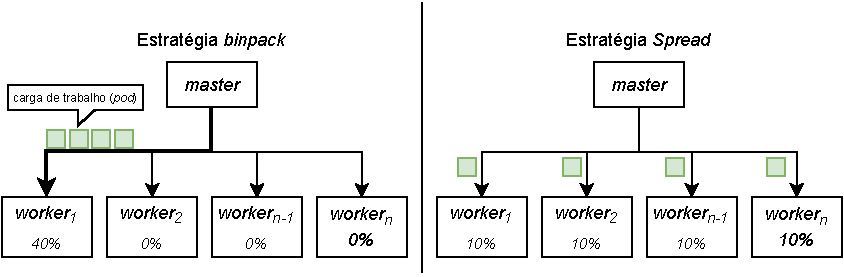
\includegraphics[width=\linewidth]{assets/distribuicao-trabalho.pdf}
%DIFDELCMD < 	\legend{Fonte: O autor}
%DIFDELCMD < \end{figure}
%DIFDELCMD < 

%DIFDELCMD < %%%
\DIFdel{Na Figura \ref{fig:distribuicao_cargas} há a implementação de duas estratégias de escalonamento}\DIFdelend : \textit{Binpack} e \textit{Spread}. \textit{Binpack} está relacionado com a minimização dos recursos, ou seja, o algoritmo selecionará o mesmo \textit{Worker} enquanto existirem recursos nessa unidade computacional - na imagem o \textit{worker$_1$} está apenas com 40\% de utilização, por isso todos os \textit{pods} estão sendo direcionados a ele. Já o \textit{Spread} possui como objetivo otimizar \DIFdelbegin \DIFdel{a utilização de }\DIFdelend \DIFaddbegin \DIFadd{o balanceamento de carga dos }\DIFaddend recursos, comumente utilizado \textit{round-robin}, \DIFdelbegin \DIFdel{é }\DIFdelend \DIFaddbegin \DIFadd{sendo }\DIFaddend possível notar que as cargas estão sendo distribuídas de forma igualitária entre os \textit{workers}.


\DIFaddbegin \begin{figure}[h!]
	\caption{\label{fig:distribuicao_cargas} \DIFaddFL{Estratégias de distribuição de cargas entre }\textit{\DIFaddFL{master}} \DIFaddFL{e }\textit{\DIFaddFL{workers}}}
	\centering
	%DIF >  \includegraphics[width=\linewidth]{figuras/schedule-proposal.png}
		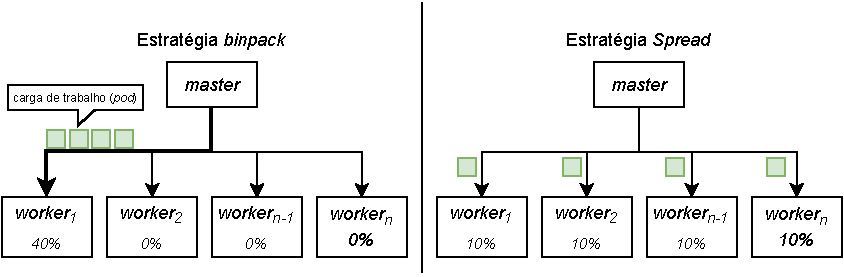
\includegraphics[width=\linewidth]{assets/distribuicao-trabalho.pdf}
	\legend{Fonte: O autor}
\end{figure}

\DIFaddend \subsection{\textit{Worker}}

O \textit{Worker} tem como objetivo resolver o escalonamento, ou seja, encontrar um \textit{node} específico para executar o \textit{pod}. A principal característica é ser um componente \textit{stateless} - não armazena estado.
Isso é possível, uma vez que foi desenvolvido no formato de microsserviço: recebe uma entrada, executa regras no escopo fechado da entrada e gera uma saída. Dessa forma, a entrada do \textit{Worker} consiste no estado atual do \textit{Cluster} e na lista de \textit{Pods}, que são informados, respectivamente, pela \textit{API} do \textit{Kubernetes} e pelo componente \textit{Master} do \ac{KMS}. Após ler a entrada são executadas operações em relação ao escalonamento, por fim, a saída representa o resultado do escalonamento. 
\DIFaddbegin 

\begin{figure}[h!]
	\caption{\label{fig:microsservico-worker} \DIFaddFL{Comparativo Microsserviço x }\textit{\DIFaddFL{Worker}}}
	\centering
	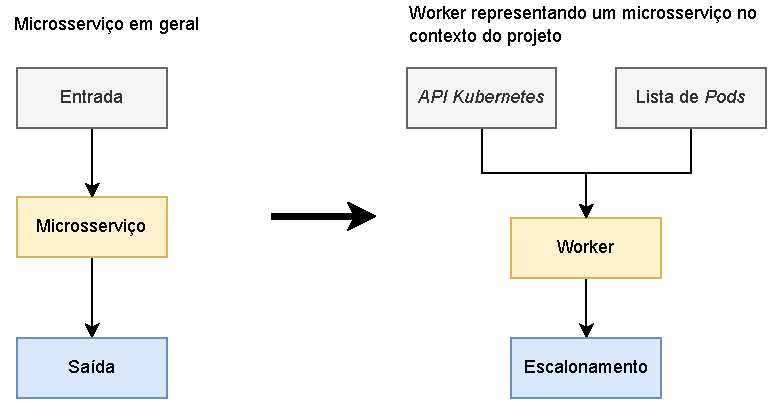
\includegraphics[width=\linewidth]{assets/microsservico-worker.pdf}
	\legend{Fonte: O autor}
\end{figure}

\DIFaddend A Figura \ref{fig:microsservico-worker} esboça o comparativo entre entre arquitetura de microsserviço genérica com o componente \textit{Worker}.
\DIFdelbegin %DIFDELCMD < 

%DIFDELCMD < \begin{figure}[h!]
%DIFDELCMD < 	%%%
%DIFDELCMD < \caption{%
{%DIFAUXCMD
%DIFDELCMD < \label{fig:microsservico-worker} %%%
\DIFdelFL{Comparativo Microsserviço x }\textit{\DIFdelFL{Worker}}%DIFAUXCMD
}
	%DIFAUXCMD
%DIFDELCMD < \centering
%DIFDELCMD < 	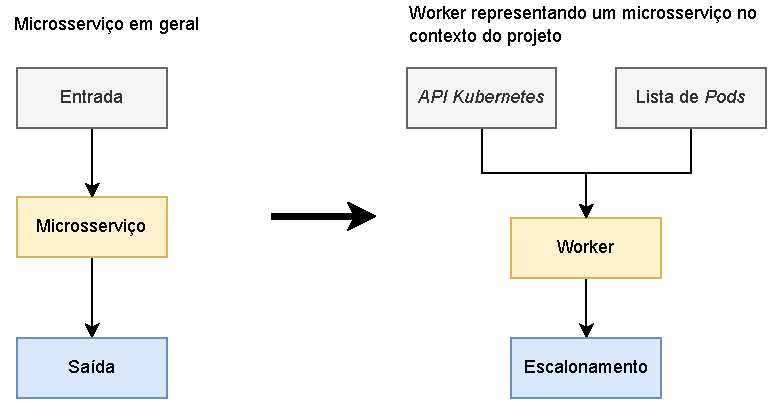
\includegraphics[width=\linewidth]{assets/microsservico-worker.pdf}
%DIFDELCMD < 	\legend{Fonte: O autor}
%DIFDELCMD < \end{figure}
%DIFDELCMD < 

%DIFDELCMD < %%%
\DIFdelend No \ac{KMS}, o \textit{Worker} é um componente com réplicas, e todas ativas. A ideia é que cada instância gerencie uma partição do \textit{cluster} \textit{Kubernetes}. Por exemplo, considere um \textit{cluster} com \textit{n} nós computacionais e \textit{w} \textit{Workers}, nesse contexto, cada instância do \textit{Worker} será responsável por $m/n$ nós do \textit{cluster}. Isto é, a instância executará o escalonamento no conjunto de nós que pertencem a sua partição.

Ao executar o \ac{KMS} em um \textit{cluster} com 6 nós computacionais e 2 instâncias do componente \textit{Worker}, o \textit{cluster} será seccionado em 2 conjuntos de nós de tamanho 3 (\textit{Tamanho Cluster} / \textit{quantidade réplicas Worker}). Logo, cada instância do \textit{Worker} será responsável por processar o escalonamento da sua respectiva partição, como demonstra a \DIFdelbegin \DIFdel{figura \ref{fig:particionamento-worker}.
}%DIFDELCMD < 

%DIFDELCMD < \begin{figure}[h!]
%DIFDELCMD < 	%%%
%DIFDELCMD < \caption{%
{%DIFAUXCMD
%DIFDELCMD < \label{fig:particionamento-worker} %%%
\DIFdelFL{particionamento do }\textit{\DIFdelFL{cluster}} %DIFAUXCMD
\DIFdelFL{entre }\textit{\DIFdelFL{workers}}%DIFAUXCMD
}
	%DIFAUXCMD
%DIFDELCMD < \centering
%DIFDELCMD < 	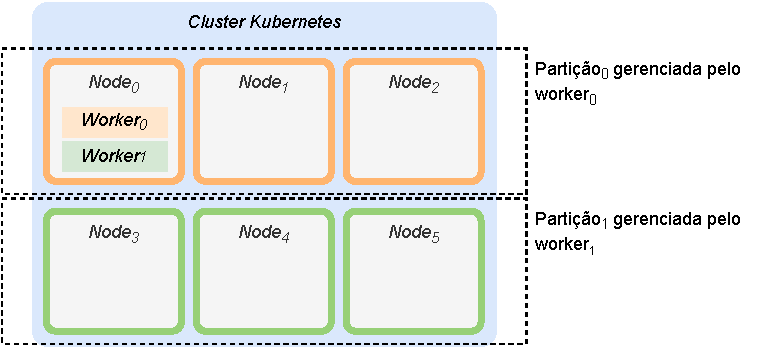
\includegraphics[width=\linewidth]{assets/particionamento-worker.pdf}
%DIFDELCMD < 	\legend{Fonte: O autor}
%DIFDELCMD < \end{figure}
%DIFDELCMD < 

%DIFDELCMD < %%%
\DIFdel{Na Figura anterior, notou-se que }\DIFdelend \DIFaddbegin \DIFadd{Figura \ref{fig:particionamento-worker}.
Especificamente, }\DIFaddend tanto o \textit{Worker$_0$} quanto o \textit{Worker$_1$} residem em \textit{Node$_0$}\DIFdelbegin \DIFdel{. Deve-se }\DIFdelend \DIFaddbegin \DIFadd{, o que deve-se }\DIFaddend ao fato que ambas as \DIFdelbegin \DIFdel{instancias }\DIFdelend \DIFaddbegin \DIFadd{instâncias }\DIFaddend foram escalonadas pelo escalonador padrão do \textit{Kubernetes}, que tomou a decisão, neste exemplo de forma hipotética, de escalonar as duas réplicas no mesmo nó computacional. Os componentes internos do \ac{KMS} são escalonados pelo escalonador padrão do \textit{Kubernetes}.

\DIFaddbegin \begin{figure}[h!]
	\caption{\label{fig:particionamento-worker} \DIFaddFL{particionamento do }\textit{\DIFaddFL{cluster}} \DIFaddFL{entre }\textit{\DIFaddFL{workers}}}
	\centering
	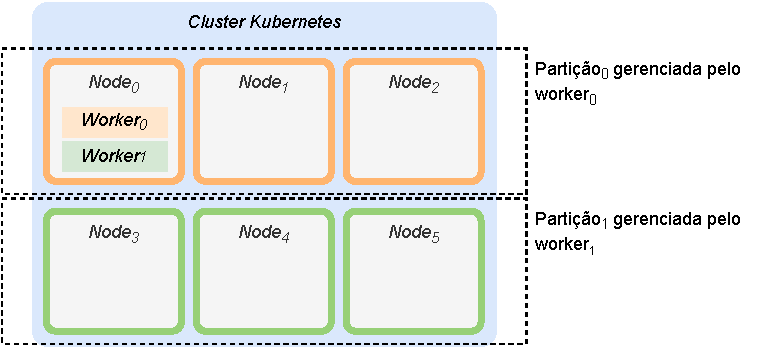
\includegraphics[width=\linewidth]{assets/particionamento-worker.pdf}
	\legend{Fonte: O autor}
\end{figure}


\DIFaddend \subsection{Relação \textit{Master}-\textit{Worker}}
As subseções anteriores se encarregaram de apresentar os componentes de forma isolada, nesta subseção objetiva-se sintetizar o funcionamento do \ac{KMS} como um todo\DIFdelbegin \DIFdel{, aqui }\DIFdelend \DIFaddbegin \DIFadd{.
Aqui, }\DIFaddend o principal objetivo é relacionar os componentes \textit{Master} e \textit{Worker}. Em resumo, o \ac{KMS} consiste em 3 passos objetivos: (1) Buscar os \textit{Pods} na fila de escalonamento interna do \textit{Kubernetes}, (2) Distribuir as cargas de trabalho entre os \textit{Workers} e (3) \DIFdelbegin \DIFdel{executar }\DIFdelend \DIFaddbegin \DIFadd{Executar }\DIFaddend o escalonamento.

\DIFdelbegin \DIFdel{Considere }\DIFdelend %DIF > no formato de microsserviço, a ideia é que cada unidade execute o escalonamento em uma partição específica do \textit{cluster}. Dessa forma, ao se executar \textit{n} \textit{workers} então o \textit{cluster} será particionado em \textit{n} partes, como esboça a Figura \ref{fig:worker}.
\DIFaddbegin 

%DIF > \begin{figure}[h!]
%DIF > 	\caption{\label{fig:worker} particionamento do \textit{cluster} entre \textit{workers}}
%DIF > 	\centering
%DIF > 	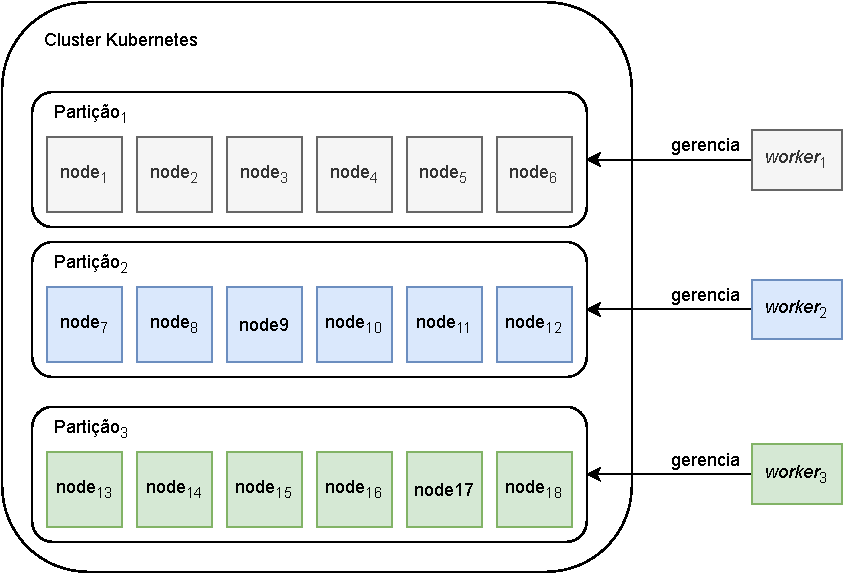
\includegraphics[width=.80\linewidth]{assets/worker.pdf}
%DIF > 	\legend{Fonte: O autor}
%DIF > \end{figure}

%DIF > A comunicação entre o sistema distribuído proposto e o \textit{Kubernetes} é efetuada pelo protocolo \ac{HTTP}, em resumo, o \textit{Kubernetes} expõe um servidor \textit{Web} que pode ser consumido por qualquer componente interno. No contexto do presente trabalho, o \textit{Master} consumirá a \textit{API} para buscar os contêineres que estão na fila de escalonamento. Na mesma linha de pensamento, o componente \textit{Worker} se comunicará com a \textit{API} para enviar ordens de escalonamento. Por outro lado, a comunicação entre o componente \textit{master} e \textit{worker} será efetivada via protocolo \textit{gRPC}. Protocolo de comunicação projetado pela \textit{Google}, a principal característica é a performance de alta velocidade entre \textit{microsserviços}.
%DIF > O fluxo de execução do sistema distribuído proposto é representado pelo diagrama de fluxo esboçado pela Figura \ref{fig:flow_diagram}.

\begin{figure}[h!]
	\caption{\label{fig:relacao-master-worker}\DIFaddFL{Diagrama de Fluxo}}
	\centering
	%DIF >  \includegraphics[width=0.3\linewidth]{figuras/schedule-proposal.png}
	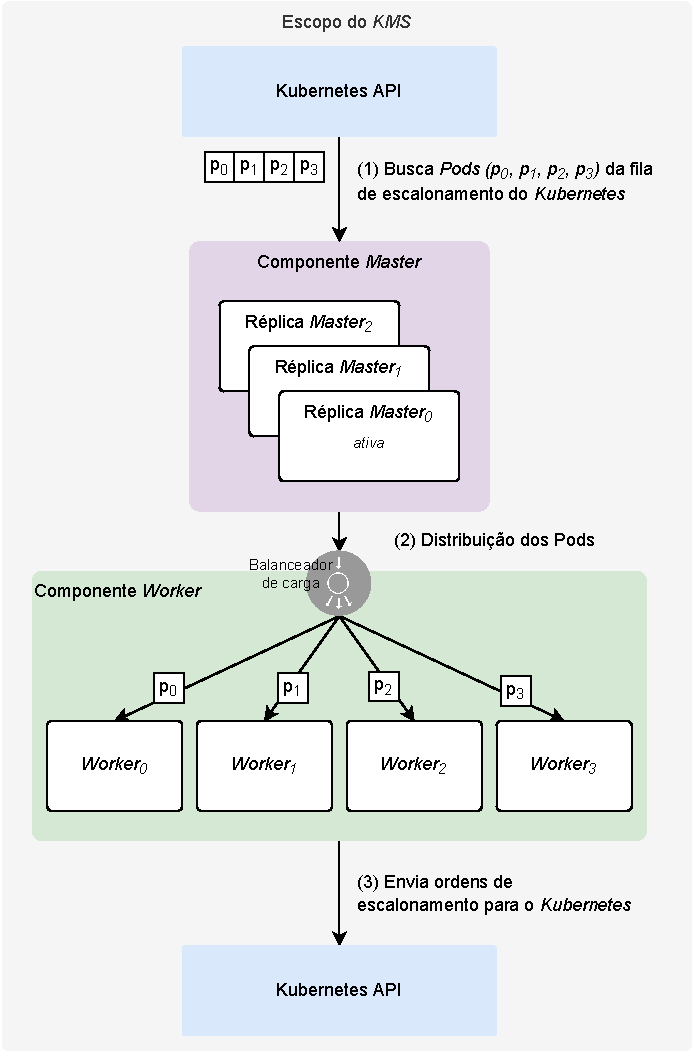
\includegraphics[width=.60\linewidth]{assets/relacao-master-worker.pdf}
	\legend{Fonte: O autor}
\end{figure}

\DIFadd{Considerando }\DIFaddend um cenário do \ac{KMS} com 3 réplicas \textit{Master} e 4 réplicas \textit{Worker}, o funcionamento do sistema distribuído proposto pode ser visualizado na Figura \ref{fig:relacao-master-worker}.
\DIFdelbegin %DIFDELCMD < 

%DIFDELCMD < %%%
%DIF < no formato de microsserviço, a ideia é que cada unidade execute o escalonamento em uma partição específica do \textit{cluster}. Dessa forma, ao se executar \textit{n} \textit{workers} então o \textit{cluster} será particionado em \textit{n} partes, como esboça a Figura \ref{fig:worker}.
%DIFDELCMD < 

%DIFDELCMD < %%%
%DIF < \begin{figure}[h!]
%DIF < 	\caption{\label{fig:worker} particionamento do \textit{cluster} entre \textit{workers}}
%DIF < 	\centering
%DIF < 	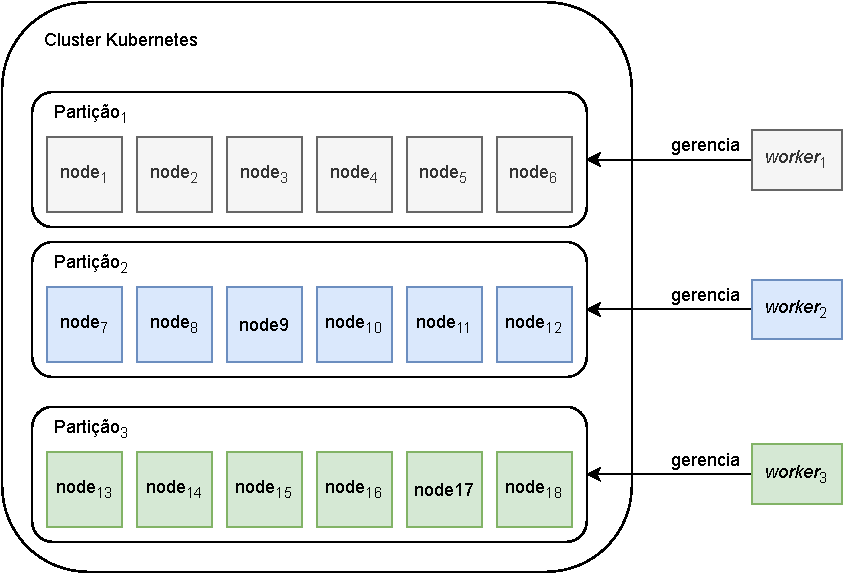
\includegraphics[width=.80\linewidth]{assets/worker.pdf}
%DIF < 	\legend{Fonte: O autor}
%DIF < \end{figure}
%DIFDELCMD < 

%DIFDELCMD < %%%
%DIF < A comunicação entre o sistema distribuído proposto e o \textit{Kubernetes} é efetuada pelo protocolo \ac{HTTP}, em resumo, o \textit{Kubernetes} expõe um servidor \textit{Web} que pode ser consumido por qualquer componente interno. No contexto do presente trabalho, o \textit{Master} consumirá a \textit{API} para buscar os contêineres que estão na fila de escalonamento. Na mesma linha de pensamento, o componente \textit{Worker} se comunicará com a \textit{API} para enviar ordens de escalonamento. Por outro lado, a comunicação entre o componente \textit{master} e \textit{worker} será efetivada via protocolo \textit{gRPC}. Protocolo de comunicação projetado pela \textit{Google}, a principal característica é a performance de alta velocidade entre \textit{microsserviços}.
%DIF < O fluxo de execução do sistema distribuído proposto é representado pelo diagrama de fluxo esboçado pela Figura \ref{fig:flow_diagram}.
%DIFDELCMD < 

%DIFDELCMD < \newpage
%DIFDELCMD < \begin{figure}[h!]
%DIFDELCMD < 	%%%
%DIFDELCMD < \caption{%
{%DIFAUXCMD
%DIFDELCMD < \label{fig:relacao-master-worker}%%%
\DIFdelFL{Diagrama de Fluxo}}
	%DIFAUXCMD
%DIFDELCMD < \centering
%DIFDELCMD < 	%%%
%DIF <  \includegraphics[width=0.3\linewidth]{figuras/schedule-proposal.png}
	%DIFDELCMD < 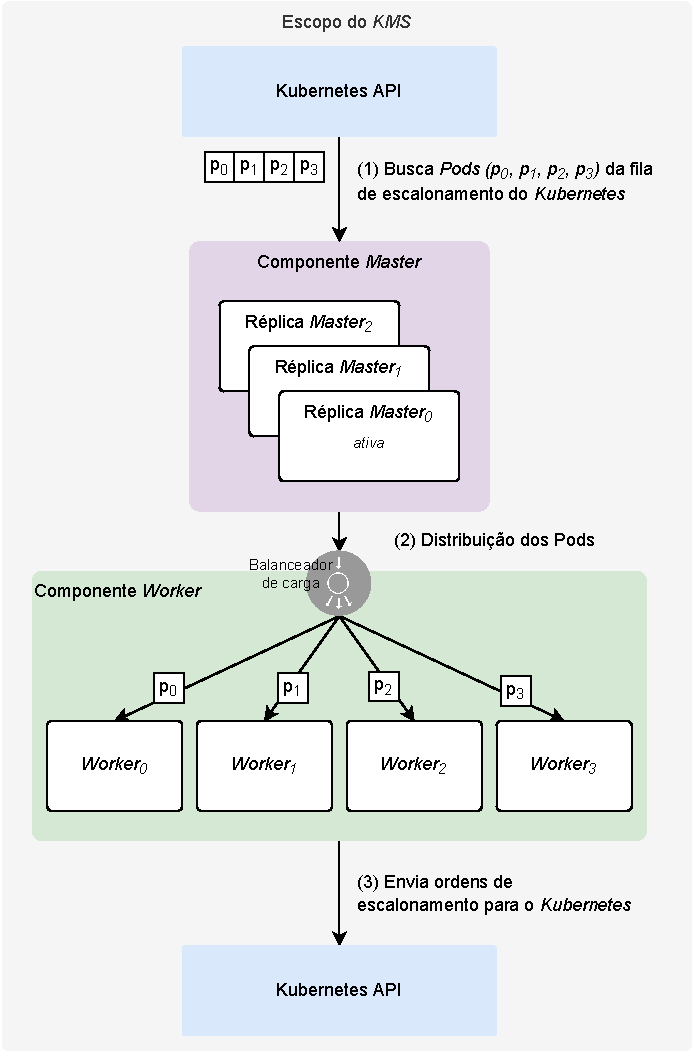
\includegraphics[width=.60\linewidth]{assets/relacao-master-worker.pdf}
%DIFDELCMD < 	\legend{Fonte: O autor}
%DIFDELCMD < \end{figure}
%DIFDELCMD < 

%DIFDELCMD < %%%
\DIFdel{O diagrama anterior }\DIFdelend %DIF > 
\DIFaddbegin \DIFadd{O diagrama }\DIFaddend apresenta a interação completa entre os módulos do \ac{KMS}, desde a coleta do \textit{Pod} pelo \textit{Master}, até o envio da ordem de escalonamento pelo \textit{Worker} para a \textit{API} do \textit{Kubernetes}. Além disso, é possível verificar que no topo do componente \textit{Worker} há um balanceador de carga, que é responsável por distribuir as requisições de escalonamento de \textit{Pods}. Com isso, o componente \textit{Master} não necessita guardar estado das instâncias do \textit{Worker}, \DIFaddbegin \DIFadd{uma vez que }\DIFaddend comunicar-se diretamente com o balanceador de carga é o suficiente. No \textit{Kubernetes} o balanceador de carga pode ser configurado tanto para a estratégia \textit{Binpack} quanto para \textit{Round-Robin}\DIFdelbegin \DIFdel{, no exemplo da imagem anterior }\DIFdelend \DIFaddbegin \DIFadd{. No exemplo da figura, }\DIFaddend a estratégia executada foi \textit{Round-Robin}. 
Outro ponto de destaque são as réplicas do componente \textit{Master}, considerado o \textbf{Produtor} do sistema distribuído, as instâncias do \textit{Master} necessitam executar algoritmo de eleição para manter apenas uma ativa executando a tarefa de \textbf{Produtor}. O algoritmo de eleição será explicitado na Seção \ref{eleicao-master}.

%Na Figura \ref{fig:flow_diagram} é exemplificado o fluxo de execução da arquitetura proposta e os papéis dos dois módulos principais: \textit{master} e \textit{worker}. O \textit{master} é responsável por buscar fila de \textit{pods} não escalonados (1) -- na figura é esboçado por $p_1, p_2, p_3, p_4, p_5, p_6, p_{n-1}, p_n$ -- e também por distribuí-los (2) aos \textit{workers} -- na figura é esboçado por $w_1, w_2, w_{n-1}, w_{n}$ --, nesta etapa foi utilizado o método de espalhamento para enviar a carga de trabalho para os \textit{workers}. Entretanto, o presente trabalho busca modularizar a arquitetura proposta de forma que possibilite intercambiar a técnica de escalonamento e utilizar, por exemplo, agrupamento ou até mesmo métodos refinados. Na etapa (2) será utilizado comunicação via \textit{gRPC}.

%No \textit{worker} há duas funções principais. A primeira é o recebimento das cargas de trabalho como é notado na figura em (2). Para isso cada unidade \textit{worker} gerencia uma fila interna que representa em ordem de chegada as cargas de trabalho enviadas pelo \textit{master}. A segunda função, a principal, é a execução do algoritmo de escalonamento que vinculará o \textit{pod} a um \textit{node}. O método de escalonamento será modular, ou seja, haverá uma lista de implementações de escalonamento pré-definida (\textit{spread, binpack, backfilling}), mas o objetivo é que seja extensível e possa executar até métodos refinados de escalonamento.

\section{Trocas de Mensagens}

A comunicação entre o sistema distribuído proposto e o \textit{Kubernetes} é efetuada pelo protocolo \ac{HTTP}\DIFdelbegin \DIFdel{, em }\DIFdelend \DIFaddbegin \DIFadd{.
Em }\DIFaddend resumo, o \textit{Kubernetes} expõe um servidor \textit{Web} que pode ser consumido por qualquer componente interno. No contexto do presente trabalho, o \textit{Master} consumirá a \textit{API} para buscar os contêineres que estão na fila de escalonamento. Na mesma linha de pensamento, o componente \textit{Worker} se comunicará com a \textit{API} para enviar ordens de escalonamento. A comunicação entre o componente \textit{Master} e \textit{Worker} também será efetivada via protocolo \ac{HTTP}, em síntese, cada instância do \textit{Worker} abrirá um servidor \textit{Web} para consumir as cargas de trabalho enviadas pelo \textit{Master}. Ao utilizar essa arquitetura, \DIFdelbegin \DIFdel{será }\DIFdelend \DIFaddbegin \DIFadd{é }\DIFaddend possível definir novas rotas para o servidor \textit{Web} do \textit{Worker}, além daquelas relacionadas ao escalonamento, como por exemplo, rotas para verificar a saúde do próprio contêiner da instância do \textit{Worker} com o objetivo de checar sobrecarga. Para elucidar as trocas de mensagens foi elaborado um diagrama de sequência com os eventos principais do \ac{KMS}, pode ser visualizado na Figura \ref{fig:sequencia}. 

\begin{figure}[h!]
	\caption{\label{fig:sequencia}Diagrama de Sequência \ac{KMS}}
	\centering
	% \includegraphics[width=0.3\linewidth]{figuras/schedule-proposal.png}
	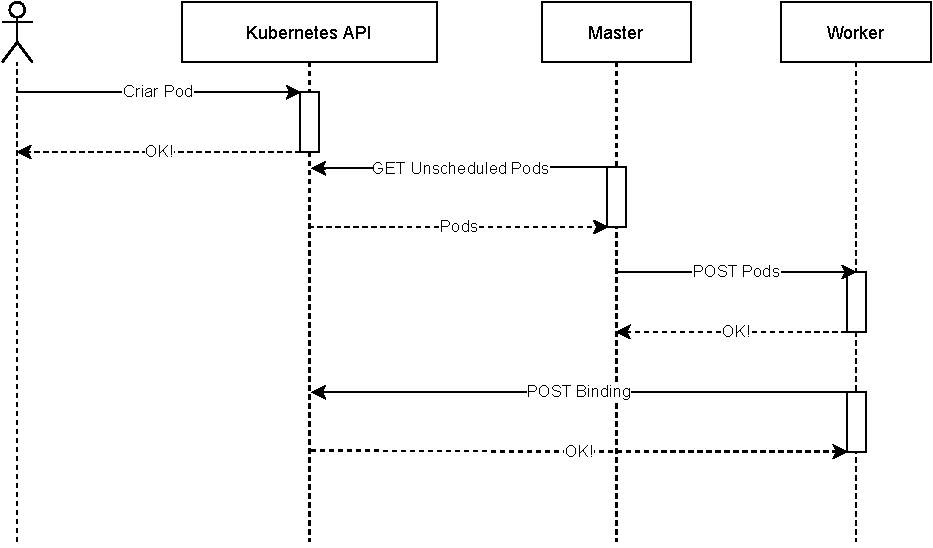
\includegraphics[width=\linewidth]{assets/sequencia.pdf}
	\legend{Fonte: O autor}
\end{figure}

Como todos os módulos do \ac{KMS} se comunicam por \textit{HTTP}, o diagrama de sequência foi elaborado utilizando a nomenclatura padrão de requisições \textit{Web} - \textit{POST e GET}. O ponto de partida é no momento em que um novo \textit{Pod} é inserido na plataforma pelo usuário, \DIFdelbegin \DIFdel{isso deve }\DIFdelend \DIFaddbegin \DIFadd{devendo }\DIFaddend ser executado obrigatoriamente pela \textit{API} do \textit{Kubernetes} \DIFdelbegin \DIFdel{, }\DIFdelend \DIFaddbegin \DIFadd{(}\DIFaddend na figura corresponde ao evento \textit{Criar Pod}\DIFaddbegin \DIFadd{)}\DIFaddend . 
Este \textit{Pod} permanecerá na fila de escalonamento interna até algum escalonador requisitar os \textit{Pods} não escalonados, que é observado no evento \textit{GET Unscheduled Pods}. O próximo passo é distribuir os \textit{Pods} para os \textit{Workers} por meio do evento \textit{POST Pods}, que é executado pelo \textit{Master}. Ao fim, o \textit{Worker} executa o escalonamento e envia uma ordem do tipo \textit{binding} para a \textit{API} do \textit{Kubernetes}, que vinculará o \textit{Pod} à algum nó eleito pelo \textit{Worker} no processo de escalonamento. Essa última etapa é representada pelo evento \textit{POST binding}.


\section{Eleição do Componente \textit{Master} \label{eleicao-master}}

Um dos princípios do \ac{KMS} é desenvolver uma aplicação distribuída sem \DIFaddbegin \DIFadd{um }\DIFaddend único ponto de falha\DIFdelbegin \DIFdel{, isso influência }\DIFdelend \DIFaddbegin \DIFadd{.
Essa abordagem influencia }\DIFaddend que todos os módulos do sistema necessitem algum tipo de controle de falhas. O módulo \textit{Worker} é representado no formato de microsserviço, e todas as suas réplicas trabalham simultaneamente, a sua natureza por sí só já possui controle de falhas. Entretanto, o módulo \textit{Master}, mencionado nas seções anteriores como \textbf{Produtor} do sistema distribuído, demanda que apenas uma réplica esteja em execução trabalhando no escalonamento. Dado o contexto, verificou-se que uma das formas de resolver este problema é utilizar algoritmo de eleição para manter apenas uma réplica do \textit{Master} executando o escalonamento enquanto o restante permaneçam em espera.

Visando simplificar o desenvolvimento, neste trabalho foi utilizado \textit{Redis}, um banco de dados em memória e distribuído, para executar o ambiente de eleição. O principal objetivo da escolha dessa tecnologia é se beneficiar da funcionalidade de \textit{Locks Distribuídos} \cite{redisDistributedLocks}. Os \textit{Locks Distribuídos} são considerados uma primitiva de banco de dados, que auxiliam em cenários onde diferentes processos operam recursos compartilhados de forma mutuamente exclusiva.

\subsection{Algoritmo de eleição apoiado no \textit{Redis}}

Em síntese, o processo de eleição, baseado em \textit{Locks Distribuídos}, consiste em reproduzir um cenário de corrida entre os processos, o primeiro que conseguir escrever a sua identificação no recurso compartilhado do \textit{Redis} será eleito líder. O campo que o líder escreveu a própria identificação possui tempo de expiração (\textit{TTL - Time To Live}), no momento em que a informação for perdida resultará em uma nova corrida entre os processos. Os passos a seguir demonstram a execução do algoritmo na prática.

\newpage
\subparagraph{Passo 1:} Todos os \textit{Masters} tentarão escrever no campo \textit{current} do Redis o próprio \textit{id}. Por exemplo, \textit{Master$_2$} tentará escrever \textit{m2} em \textit{current}. O campo \textit{current} foi configurado para ser compartilhado de forma mutuamente exclusiva. Este passo é visualizado na figura \ref{fig:eleicao-passo-1}

\begin{figure}[h!]
	\caption{\label{fig:eleicao-passo-1}Passo 1 eleição}
	\centering
	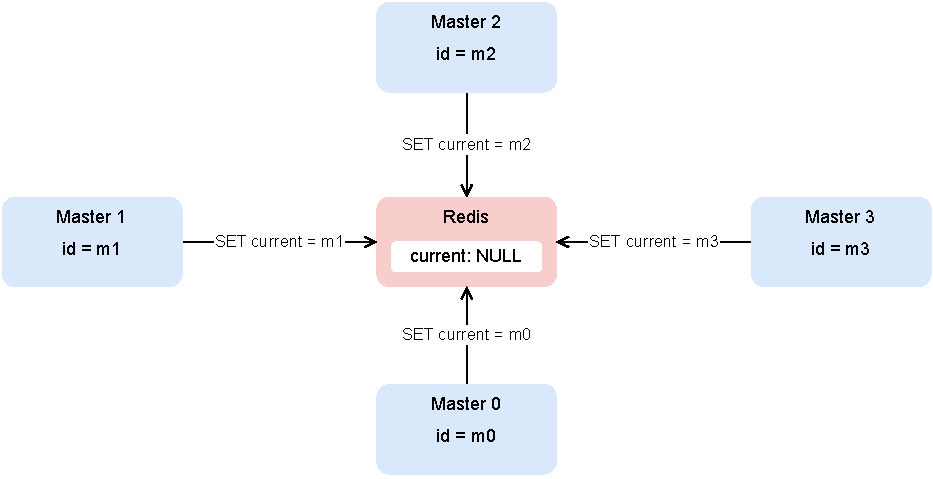
\includegraphics[width=.6\linewidth]{assets/eleicao-passo-1.pdf}
	\legend{Fonte: O autor}
\end{figure}

\subparagraph{Passo 2:} \textit{Redis} vai utilizar \textit{lock} interno e apenas uma instância do \textit{Master} vai conseguir escrever o id no campo \textit{current}. Só é possível escrever se o campo current for nulo. Nesse exemplo, \textit{Master$_2$} foi premiado e tournou-se líder. Este passo é visualizado na figura \ref{fig:eleicao-passo-2}.

\begin{figure}[h!]
	\caption{\label{fig:eleicao-passo-2}Passo 2 eleição}
	\centering
	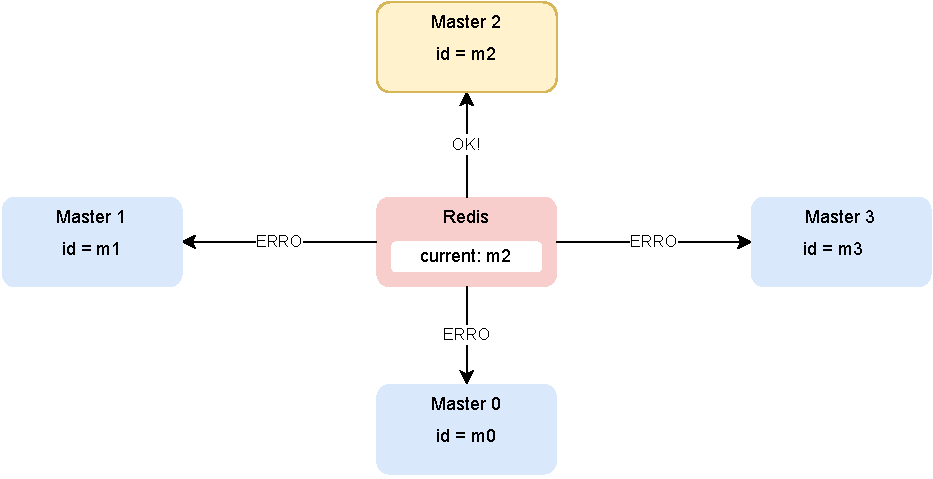
\includegraphics[width=.6\linewidth]{assets/eleicao-passo-2.pdf}
	\legend{Fonte: O autor}
\end{figure}

\subparagraph{Passo 3:} O \textit{Redis} está configurado para cada 4 segundos o campo \textit{current} voltar a ser nulo e permitir a corrida entre os \textit{Masters}. Entretanto, o líder, no caso \textit{Master$_2$}, a cada intervalo de 2 segundos aumentará o \textit{TTL} do campo \textit{current} em 4 segundos. Este passo é visualizado na figura \ref{fig:eleicao-passo-3}.

\begin{figure}[h!]
	\caption{\label{fig:eleicao-passo-3}Passo 3 eleição}
	\centering
	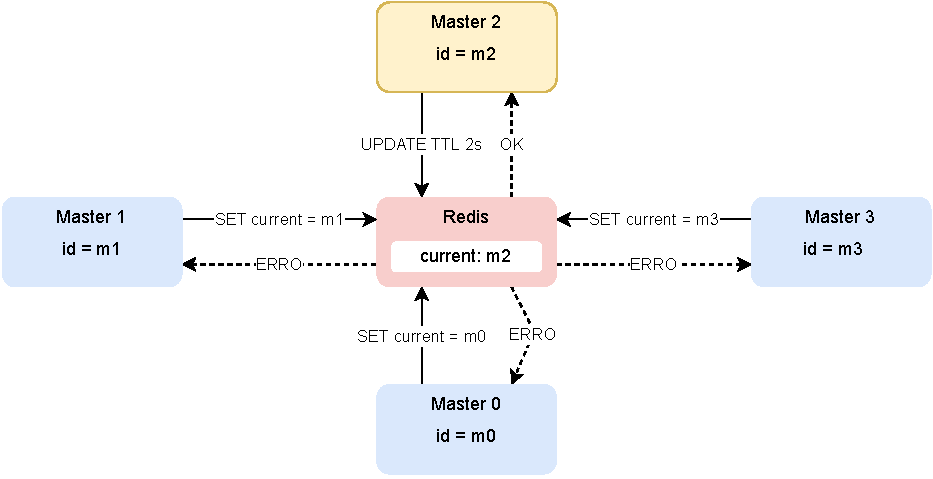
\includegraphics[width=.6\linewidth]{assets/eleicao-passo-3.pdf}
	\legend{Fonte: O autor}
\end{figure}

\subparagraph{Passo 4:} Considere que o \textit{Master$_2$} perdeu a conexão ou foi derrubado. Ou seja, não irá conseguir atualizar o \textit{TTL} do valor \textit{current}. Portanto, em 4 segundos o valor \textit{current} voltará a ser nulo e permitira a corrida entre os \textit{Masters}. Este passo é visualizado na figura \ref{fig:eleicao-passo-4}.

\begin{figure}[h!]
	\caption{\label{fig:eleicao-passo-4}Passo 4 eleição}
	\centering
	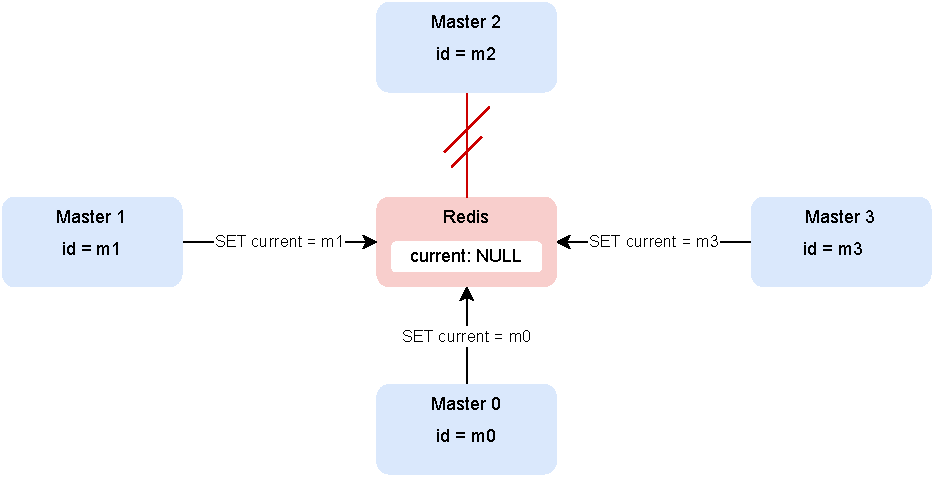
\includegraphics[width=.6\linewidth]{assets/eleicao-passo-4.pdf}
	\legend{Fonte: O autor}
\end{figure}

\subparagraph{Passo 5:} Como o campo \textit{current} voltou a ser nulo, uma nova corrida é executada. Considere que o \textit{Master$_1$} conseguiu escrever \textit{m1} em \textit{current} e será o novo líder e responsável por atualizar o \textit{TTL} enquanto ainda estiver disponível. Este passo é visualizado na figura \ref{fig:eleicao-passo-5}.

\begin{figure}[h!]
	\caption{\label{fig:eleicao-passo-5}Passo 5 eleição}
	\centering
	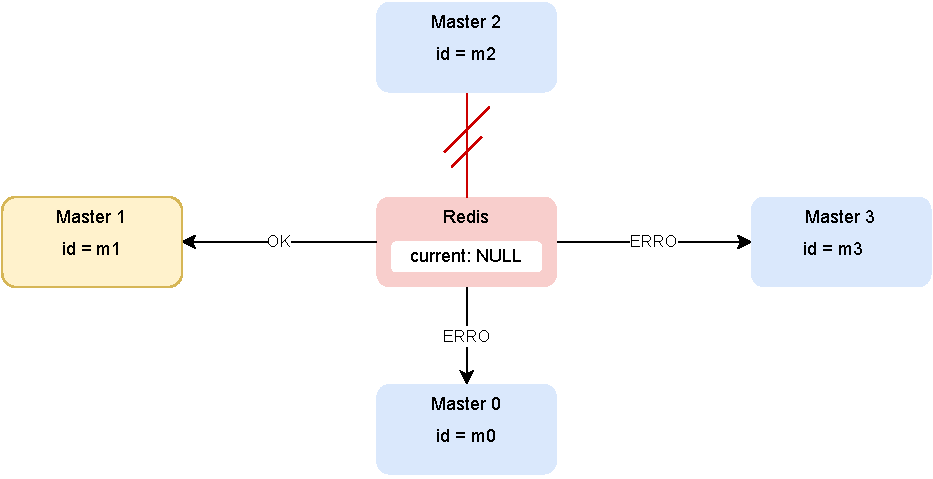
\includegraphics[width=.6\linewidth]{assets/eleicao-passo-5.pdf}
	\legend{Fonte: O autor}
\end{figure}



\newpage
\section{Implantação em \textit{Kubernetes}}
A arquitetura proposta é executada no topo do \textit{Kubernetes}, dessa forma, os componentes principais são conteinerizados e provisionados pelo próprio \textit{Kubernetes}. Na Seção 2.2.4 foram apresentadas 4 formas distintas de customizar o escalonador padrão, após analisar a viabilidade, chegou-se a conclusão que o método \textbf{Múltiplos escalonadores} é o ideal para a implementação do projeto. Essa abordagem consiste no desenvolvimento de um escalonador que é executado no formato de \textit{Pod} e toda a comunicação com o \textit{Kubernetes} é realizada via troca de mensagens por meio da \textit{API}. Com isso, o componente \textit{Worker} torna-se completamente \textit{stateless}, pois o estado do \textit{cluster} é mantido pelo próprio \textit{Kubernetes}. Neste contexto, o problema de escalonamento, na visão do \textit{Worker}, é da forma entrada e saída: a entrada é o estado do \textit{cluster} que é informado pela \textit{API}, a saída é a ação de escalonamento efetuada pelo \textit{Worker}. Portanto, o escalonador proposto será executado ao lado do escalonador padrão e representado por um conjunto de \textit{pods}. A Figura \ref{fig:proposta_kubernetes} demonstra um caso de uso com 2 instâncias de \textit{Workers} que coordenam o escalonamento de 2 \textit{Nodes} do \textit{Kubernetes}, o \textit{Worker$_0$} é responsável pelo \textit{Node$_0$} e \textit{Node$_2$} (cor roxa) já o \textit{Worker$_1$} pelo \textit{Node$_1$} e \textit{Node$_3$} (cor amarela).

\begin{figure}[h!]
	\caption{\label{fig:proposta_kubernetes}Exemplo de implantação.}
	\centering
	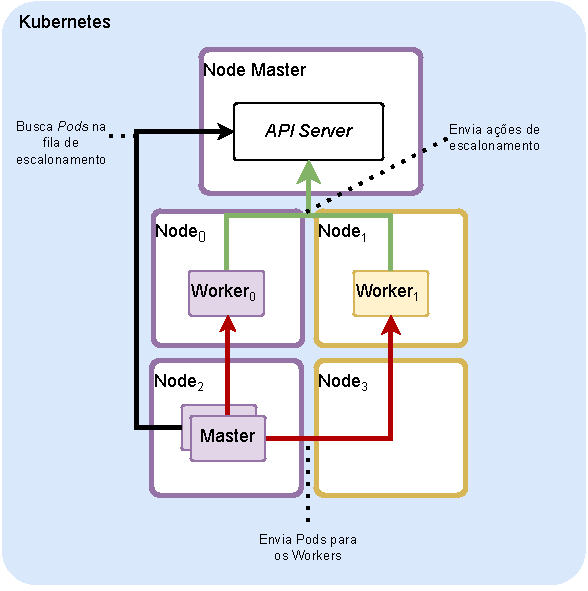
\includegraphics[width=.7\linewidth]{assets/arquitetura-worker.pdf}
	\legend{Fonte: O autor}
\end{figure}

Na figura percebe-se que as instâncias do componente \textit{Master} residem no \textit{Node$_2$}, isso se deve ao fato que as instâncias dos componentes do \ac{KMS} são conteinerizados e escalonadas pelo escalonador padrão do \textit{Kubernetes}. Logo, não é tarefa do escalonador proposto pré definir os nodes em que as próprias instâncias serão executadas, isso é tarefa do \textit{Kubernetes} por meio do escalonador padrão.

Ao utilizar o método de múltiplos escalonadores, no momento de provisionar um novo \textit{pod} para a plataforma é necessário discriminar o escalonador desejado, que é possível por meio do atributo \textit{schedulerName}. Isso é alterado facilmente no arquivo de manifesto do \textit{pod}, como ilustra a Figura \ref{fig:pod_custom_scheduler}.

\begin{figure}[h!]
	\caption{\label{fig:pod_custom_scheduler}Direcionamento do \textit{pod} para o escalonador \textit{my-scheduler}}
	\centering
	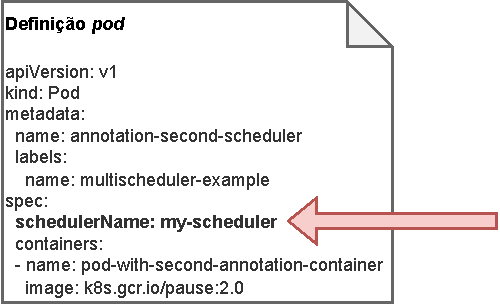
\includegraphics[width=0.6\linewidth]{assets/pod-custom-scheduler.pdf}
	\legend{Fonte: O autor}
\end{figure}

\newpage
\section{Representação por Diagramas de Classes}

O diagrama de classes da proposta é visualizado pelas figuras \ref{fig:worker_class_diagram} e \ref{fig:master_class_diagram}. No diagrama do \textit{Worker} é utilizado o padrão de projeto \textit{strategy} para alternar o método de escalonamento, além disso, há também outros dois métodos -- \textit{solve} e \textit{binding}. \textit{Solve} é responsável por resolver o escalonamento de acordo com a estratégia escolhida, e \textit{binding} tem como objetivo enviar uma ordem de escalonamento para \textit{Kubernetes} utilizando a \textit{API}.

\subsection{Worker}
\begin{figure}[h!]
	\caption{\label{fig:worker_class_diagram}Diagrama de Classes \textit{worker}}
	\centering
	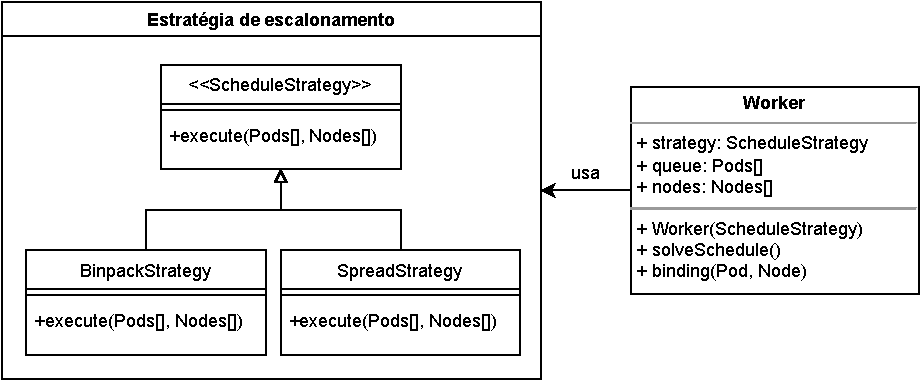
\includegraphics[width=1\linewidth]{assets/worker-class-diagram.pdf}
	\legend{Fonte: O autor}
\end{figure}

\subparagraph{Interface \textit{ScheduleStrategy}:}
Implementação do padrão de projeto \textit{Strategy}, permite intercambiar o método de escalonamento.

\subparagraph{Classe \textit{BinpackStrategy}:}
Executa o escalonamento utilizando técnica de agrupamento.

\subparagraph{Classe \textit{SpreadStrategy}:}
Executa o escalonamento utilizando técnica de espalhamento.

\subparagraph{Classe \textit{Worker}:}
Executa o escalonamento a partir da estratégia selecionada. A estratégia é escolhida no método de construção da classe \textit{Worker(ScheduleStrategy)}. Também há a especificação da fila de escalonamento representado pelo atributo \textit{queue} e dos nós -- \textit{nodes} -- que o \textit{Worker} está gerenciando. O método \textit{solveSchedule} executa o escalonamento a partir da estratégia selecionada e \textit{binding} envia ordem de escalonamento para \textit{API} do \textit{Kubernetes}.

\subsection{Master}
\begin{figure}[h!]
	\caption{\label{fig:master_class_diagram}Diagrama de Classes \textit{Master}}
	\centering
	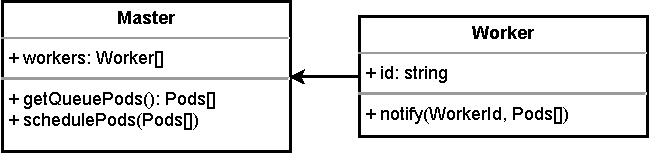
\includegraphics[width=0.65\linewidth]{assets/master-class-diagram.pdf}
	\legend{Fonte: O autor}
\end{figure}

\subparagraph{Classe \textit{Worker}:}
Representa a entidade \textit{Worker} no escopo do \textit{Master}. Em resumo, consiste em um atributo para identificação -- \textit{id} -- e um método para a comunicação de envio dos \textit{Pod} denominado \textit{notify}.

\subparagraph{Classe \textit{Master}:}
Possui uma lista de \textit{Workers} vinculado, é responsável por buscar os \textit{Pods} que estão na fila de escalonamento do \textit{Kubernetes} -- \textit{getQueuePods}. Já o método \textit{schedulePods} objetiva-se executar o particionamento e direcionar cada parte da fila de escalonamento para um \textit{Worker} específico.

\section{Considerações parciais}
A proposta aqui elucidada visa o projeto de uma arquitetura distribuída, fundamentada em microsserviços, para a plataforma \textit{Kubernetes}. Isso caracteriza um projeto multidisciplinar, pois fundamentos de engenharia de software são essenciais para levantamento de requisitos, documentação em \textit{UML} e na identificação e construção dos microsserviços. Além disso, o desenvolvimento de sistemas hierárquicos está relacionado com a grande área de sistemas distribuídos, conceitos esses, essenciais na construção da arquitetura replicável dos módulos \textit{master}-\textit{worker}. Classifica-se também um projeto em redes de computadores, pois todas as interações entre os serviços se dão via comunicação, seja entre os microsserviços utilizando o protocolo \textit{gRPC} e até mesmo com o próprio \textit{Kubernetes} que é utilizado \ac{HTTP}.






% ----------------------------------------------------------

% ----------------------------------------------------------
% Análise Experimental
% ----------------------------------------------------------
\chapter{Análise Experimental}
Nesta seção objetiva-se definir os detalhes de infraestrutura do ambiente de testes, isso inclui as versões dos sistemas que serão utilizados, tanto o \textit{Kubernetes} quanto sistema operacional das unidades computacionais. Outro ponto a salientar é a definição dos parâmetros e as métricas de interesse, como também a carga de trabalho que irá estressar a arquitetura no ambiente de testes.

\section{Ambiente experimental}
Para ambiente experimental será utilizada a Nuvem da UDESC, com isso, os \textit{nodes} serão máquinas virtuais gerenciadas pelo \textit{Openstack}. Quanto ao sistema operacional não há muita influência no decorrer do presente trabalho, pois o único requisito do \textit{Kubernetes} na versão \textit{v1.23} é que o \textit{node} seja executado em ambiente \textit{linux}, portanto, o \ac{SO} escolhido será \textit{ubuntu cloud} que é projetado para nuvem. A princípio, os \textit{nodes} serão munidos por máquinas virtuais com recurso limitado em 4 núcleos e 4 gigas de memória \textit{RAM}. A principal motivação para a escolha dessa configuração está nos testes, os quais projetaremos com foco em cargas de trabalho com processamento exaustivo.

\section{}{Parâmetros e métricas}
Um dos principais desafios do presente trabalho é investigar e definir os parâmetros da arquitetura proposta. A princípio, há dois parâmetros inicias os quais serão desenvolvidos: (1) variação no número de réplicas do escalonador e (2) quantidade de \textit{nodes} do \textit{cluster} que cada \textit{worker} gerenciará. No contexto do presente trabalho, em (1) será variado em diversas rodadas de testes, será considerado de início apenas 2 réplicas e subir a quantidade gradativamente até atingir o limite físico da arquitetura. Já (2) possui um nível de complexidade maior que (1), a forma natural é dividir de forma proporcional, por exemplo, em um \textit{cluster} com 10 \textit{nodes} e 5 \textit{workers} então cada \textit{worker} gerenciará 2 \textit{nodes}. Contudo, de acordo com a literatura, esse é um parâmetro que há margem de refinamento. Considera-se o trabalho de \citeonline{vaucher2018sgxaware}, o qual consiste em escalonamento em \textit{cluster} heterogêneo -- máquinas com diferentes arquiteturas e capacidades de processamento. Neste cenário, não seria interessante utilizar o método proporcional de divisão entre \textit{workers} e \textit{nodes}. Outro exemplo é o trabalho de \citeonline{Wang2019Pigeon}, o qual consiste em particionar o \textit{cluster} de acordo com a complexidade das cargas de trabalho. Este trabalho considerou que cargas de trabalho menores deveriam ser executadas em um segmento do \textit{cluster} diferente que cargas de trabalhos consideradas complexas. Neste cenário houve acréscimo do desempenho na métrica de tempo de espera.

As métricas de interesse do presente trabalho estão relacionadas com o desempenho de escalonamento, assim, o desempenho está diretamente relacionado com o tempo de espera de escalonamento. Quanto menos tempo uma carga de trabalho permanecer na fila maior é o desempenho da proposta de escalonamento. Portanto, há duas métricas que serão avaliadas de acordos com os parâmetros propostos: tempo de espera de escalonamento e \textit{makespan}. As métricas de sobrecarga também serão importantes, principalmente relacionadas a sobrecarga do \textit{node}, seja de espaço ou processamento.
% ----------------------------------------------------------

% ----------------------------------------------------------
% Proposta
% ----------------------------------------------------------
\chapter{Conclusão}

Escalonamento é considerado um processo de tomada de decisão, em resumo, no contexto do presente trabalho, o objetivo é alocar contêineres em nós computacionais denominados \textit{nodes} com recursos finito. Há diversos parâmetros a ser considerados, por consequência, é possível alcançar as mais divergentes funções objetivos -- reduzir consumo energético, otimizar utilização de recursos do \textit{data center}. Logo, de maneira geral, os algoritmos de otimização de escalonamento se enquadram na classe \textit{NP-difícil} \cite{ullman1975np}, visto que, a natureza do problema de escalonamento é combinatória.

A explosão da demanda de poder computacional dos \textit{data centers} uniram, ainda mais, as áreas entre escalonamento e sistemas distribuídos. O objetivo desse trabalho, é, a partir da intersecção entre as duas áreas, resolver de forma elegante o problema de escalonamento para \textit{data centers} de larga escala. De acordo com a literatura, \textit{data centers} de larga escala necessitam de componentes internos sofisticados e adaptáveis que lidam com o gerenciamento de centenas de milhares de cargas de trabalho. Assim, a construção de uma arquitetura de escalonamento distribuída, até o momento, é a solução para que as empresas, como \textit{Google} e \textit{Microsoft}, tratem um grande volume de requisições de escalonamento \cite{Wang2019Pigeon, Google2015Borg}.

Ao unir as áreas entre sistemas distribuídos e escalonamento encontra-se quantidade significativa de estudos explorados, entretanto, a intersecção entre essas áreas junto com orquestradores de contêineres é escasso na literatura como visto no Capítulo 3. Este trabalho possui como objetivo suprir essa carência, uma vez que a principal arquitetura de escalonamento encontrada em \textit{data centers} de larga escala, atualmente, é distribuída. Para validação da proposta, os resultados da arquitetura aqui desenvolvida serão comparados com o escalonador padrão do \textit{Kubernetes}. Com isso, objetiva-se chegar no resultado positivo, cujo as métricas de tempo de espera de escalonamento e \textit{makespan} sejam reduzidas. Além disso, haverá um estudo relacionado ao comportamento da métrica de \textit{slowdown} nos dois cenários propostos: escalonamento padrão e distribuído.


\section{Trabalhos futuros}
\noindent
A seguir é exposto as etapas de desenvolvimento do projeto, considerando em \textbf{\textcolor{green}{verde}} as etapas que já foram concluída no período esperado e em \textbf{preto} as etapas a ser desenvolvidas. 

\begin{enumerate}
	\item Revisão bibliográfica sobre contêineres e escalonamento;
	\item Estudo sobre orquestração de contêineres;
	\item Elaboração teórica do algoritmo de escalonamento proposto;
	\item Implementação do algoritmo desenvolvido no gerenciador de contêiner;

	\item Redação TCC-I;
	\item Ajustes de implementação;
	\item Desenvolver definições de análise;
	\item Análise e comparação dos resultados; e
	\item Redação TCC-II.
\end{enumerate}
% Please add the following required packages to your document preamble:
% \usepackage{multirow}
% \usepackage[table,xcdraw]{xcolor}
% If you use beamer only pass "xcolor=table" option, i.e. \documentclass[xcolor=table]{beamer}
% Please add the following required packages to your document preamble:
% \usepackage{multirow}
% \usepackage[table,xcdraw]{xcolor}
% If you use beamer only pass "xcolor=table" option, i.e. \documentclass[xcolor=table]{beamer}
\begin{table}[h]
\centering
	\caption{\label{tab:calendario_cronograma}Calendário cronograma}
	\begin{tabular}{|c|cccccccccccc|cccccccccccc|}
		\hline
		& \multicolumn{12}{c|}{2021/2}                                                                                                                                                                                                                                                                                                                                                                                                                                                                                                                     & \multicolumn{12}{c|}{2022/1}                                                                                                                                                                                                                                                                                                                                                                                                                                                                                                                     \\ \cline{2-25} 
		\multirow{-2}{*}{Etapas} & \multicolumn{2}{c|}{O}                                                & \multicolumn{2}{c|}{N}                                                                        & \multicolumn{2}{c|}{D}                                                                        & \multicolumn{2}{c|}{J}                                                                        & \multicolumn{2}{c|}{F}                                                                        & \multicolumn{2}{c|}{M}                                                   & \multicolumn{2}{c|}{A}                                                                        & \multicolumn{2}{c|}{M}                                                                        & \multicolumn{2}{c|}{J}                                                                        & \multicolumn{2}{c|}{J}                                                                        & \multicolumn{2}{c|}{A}                                                                        & \multicolumn{2}{c|}{S}                           \\ \hline
		1                        & \multicolumn{1}{c|}{} & \multicolumn{1}{c|}{\cellcolor[HTML]{009901}} & \multicolumn{1}{c|}{\cellcolor[HTML]{009901}} & \multicolumn{1}{c|}{\cellcolor[HTML]{009901}} & \multicolumn{1}{c|}{\cellcolor[HTML]{009901}} & \multicolumn{1}{c|}{}                         & \multicolumn{1}{c|}{}                         & \multicolumn{1}{c|}{}                         & \multicolumn{1}{c|}{}                         & \multicolumn{1}{c|}{}                         & \multicolumn{1}{c|}{}                         &                          & \multicolumn{1}{c|}{}                         & \multicolumn{1}{c|}{}                         & \multicolumn{1}{c|}{}                         & \multicolumn{1}{c|}{}                         & \multicolumn{1}{c|}{}                         & \multicolumn{1}{c|}{}                         & \multicolumn{1}{c|}{}                         & \multicolumn{1}{c|}{}                         & \multicolumn{1}{c|}{}                         & \multicolumn{1}{c|}{}                         & \multicolumn{1}{c|}{}                         &  \\ \hline
		2                        & \multicolumn{1}{c|}{} & \multicolumn{1}{c|}{}                         & \multicolumn{1}{c|}{\cellcolor[HTML]{009901}} & \multicolumn{1}{c|}{\cellcolor[HTML]{009901}} & \multicolumn{1}{c|}{\cellcolor[HTML]{009901}} & \multicolumn{1}{c|}{\cellcolor[HTML]{009901}} & \multicolumn{1}{c|}{}                         & \multicolumn{1}{c|}{}                         & \multicolumn{1}{c|}{}                         & \multicolumn{1}{c|}{}                         & \multicolumn{1}{c|}{}                         &                          & \multicolumn{1}{c|}{}                         & \multicolumn{1}{c|}{}                         & \multicolumn{1}{c|}{}                         & \multicolumn{1}{c|}{}                         & \multicolumn{1}{c|}{}                         & \multicolumn{1}{c|}{}                         & \multicolumn{1}{c|}{}                         & \multicolumn{1}{c|}{}                         & \multicolumn{1}{c|}{}                         & \multicolumn{1}{c|}{}                         & \multicolumn{1}{c|}{}                         &  \\ \hline
		3                        & \multicolumn{1}{c|}{} & \multicolumn{1}{c|}{}                         & \multicolumn{1}{c|}{}                         & \multicolumn{1}{c|}{\cellcolor[HTML]{009901}} & \multicolumn{1}{c|}{\cellcolor[HTML]{009901}} & \multicolumn{1}{c|}{\cellcolor[HTML]{009901}} & \multicolumn{1}{c|}{\cellcolor[HTML]{009901}} & \multicolumn{1}{c|}{\cellcolor[HTML]{009901}} & \multicolumn{1}{c|}{\cellcolor[HTML]{343434}} & \multicolumn{1}{c|}{}                         & \multicolumn{1}{c|}{}                         &                          & \multicolumn{1}{c|}{}                         & \multicolumn{1}{c|}{}                         & \multicolumn{1}{c|}{}                         & \multicolumn{1}{c|}{}                         & \multicolumn{1}{c|}{}                         & \multicolumn{1}{c|}{}                         & \multicolumn{1}{c|}{}                         & \multicolumn{1}{c|}{}                         & \multicolumn{1}{c|}{}                         & \multicolumn{1}{c|}{}                         & \multicolumn{1}{c|}{}                         &  \\ \hline
		4                        & \multicolumn{1}{c|}{} & \multicolumn{1}{c|}{}                         & \multicolumn{1}{c|}{}                         & \multicolumn{1}{c|}{}                         & \multicolumn{1}{c|}{}                         & \multicolumn{1}{c|}{}                         & \multicolumn{1}{c|}{}                         & \multicolumn{1}{c|}{\cellcolor[HTML]{FFFFFF}} & \multicolumn{1}{c|}{\cellcolor[HTML]{343434}} & \multicolumn{1}{c|}{\cellcolor[HTML]{343434}} & \multicolumn{1}{c|}{\cellcolor[HTML]{343434}} & \cellcolor[HTML]{343434} & \multicolumn{1}{c|}{\cellcolor[HTML]{343434}} & \multicolumn{1}{c|}{\cellcolor[HTML]{343434}} & \multicolumn{1}{c|}{\cellcolor[HTML]{343434}} & \multicolumn{1}{c|}{\cellcolor[HTML]{343434}} & \multicolumn{1}{c|}{}                         & \multicolumn{1}{c|}{}                         & \multicolumn{1}{c|}{}                         & \multicolumn{1}{c|}{}                         & \multicolumn{1}{c|}{}                         & \multicolumn{1}{c|}{}                         & \multicolumn{1}{c|}{}                         &  \\ \hline
		5                        & \multicolumn{1}{c|}{} & \multicolumn{1}{c|}{\cellcolor[HTML]{009901}} & \multicolumn{1}{c|}{\cellcolor[HTML]{009901}} & \multicolumn{1}{c|}{\cellcolor[HTML]{009901}} & \multicolumn{1}{c|}{\cellcolor[HTML]{009901}} & \multicolumn{1}{c|}{\cellcolor[HTML]{009901}} & \multicolumn{1}{c|}{\cellcolor[HTML]{009901}} & \multicolumn{1}{c|}{\cellcolor[HTML]{009901}} & \multicolumn{1}{c|}{\cellcolor[HTML]{FFFFFF}} & \multicolumn{1}{c|}{\cellcolor[HTML]{FFFFFF}} & \multicolumn{1}{c|}{\cellcolor[HTML]{FFFFFF}} & \cellcolor[HTML]{FFFFFF} & \multicolumn{1}{c|}{}                         & \multicolumn{1}{c|}{}                         & \multicolumn{1}{c|}{}                         & \multicolumn{1}{c|}{}                         & \multicolumn{1}{c|}{}                         & \multicolumn{1}{c|}{}                         & \multicolumn{1}{c|}{}                         & \multicolumn{1}{c|}{}                         & \multicolumn{1}{c|}{}                         & \multicolumn{1}{c|}{}                         & \multicolumn{1}{c|}{}                         &  \\ \hline
		6                        & \multicolumn{1}{c|}{} & \multicolumn{1}{c|}{}                         & \multicolumn{1}{c|}{}                         & \multicolumn{1}{c|}{}                         & \multicolumn{1}{c|}{}                         & \multicolumn{1}{c|}{}                         & \multicolumn{1}{c|}{}                         & \multicolumn{1}{c|}{}                         & \multicolumn{1}{c|}{}                         & \multicolumn{1}{c|}{}                         & \multicolumn{1}{c|}{}                         &                          & \multicolumn{1}{c|}{}                         & \multicolumn{1}{c|}{}                         & \multicolumn{1}{c|}{}                         & \multicolumn{1}{c|}{}                         & \multicolumn{1}{c|}{\cellcolor[HTML]{343434}} & \multicolumn{1}{c|}{\cellcolor[HTML]{343434}} & \multicolumn{1}{c|}{\cellcolor[HTML]{343434}} & \multicolumn{1}{c|}{}                         & \multicolumn{1}{c|}{}                         & \multicolumn{1}{c|}{}                         & \multicolumn{1}{c|}{}                         &  \\ \hline
		7                        & \multicolumn{1}{c|}{} & \multicolumn{1}{c|}{}                         & \multicolumn{1}{c|}{}                         & \multicolumn{1}{c|}{}                         & \multicolumn{1}{c|}{}                         & \multicolumn{1}{c|}{}                         & \multicolumn{1}{c|}{}                         & \multicolumn{1}{c|}{}                         & \multicolumn{1}{c|}{}                         & \multicolumn{1}{c|}{}                         & \multicolumn{1}{c|}{}                         &                          & \multicolumn{1}{c|}{}                         & \multicolumn{1}{c|}{}                         & \multicolumn{1}{c|}{}                         & \multicolumn{1}{c|}{}                         & \multicolumn{1}{c|}{}                         & \multicolumn{1}{c|}{}                         & \multicolumn{1}{c|}{\cellcolor[HTML]{343434}} & \multicolumn{1}{c|}{\cellcolor[HTML]{343434}} & \multicolumn{1}{c|}{\cellcolor[HTML]{343434}} & \multicolumn{1}{c|}{}                         & \multicolumn{1}{c|}{}                         &  \\ \hline
		8                        & \multicolumn{1}{c|}{} & \multicolumn{1}{c|}{}                         & \multicolumn{1}{c|}{}                         & \multicolumn{1}{c|}{}                         & \multicolumn{1}{c|}{}                         & \multicolumn{1}{c|}{}                         & \multicolumn{1}{c|}{}                         & \multicolumn{1}{c|}{}                         & \multicolumn{1}{c|}{}                         & \multicolumn{1}{c|}{}                         & \multicolumn{1}{c|}{}                         &                          & \multicolumn{1}{c|}{}                         & \multicolumn{1}{c|}{}                         & \multicolumn{1}{c|}{}                         & \multicolumn{1}{c|}{}                         & \multicolumn{1}{c|}{}                         & \multicolumn{1}{c|}{}                         & \multicolumn{1}{c|}{}                         & \multicolumn{1}{c|}{\cellcolor[HTML]{343434}} & \multicolumn{1}{c|}{\cellcolor[HTML]{343434}} & \multicolumn{1}{c|}{\cellcolor[HTML]{343434}} & \multicolumn{1}{c|}{}                         &  \\ \hline
		9                        & \multicolumn{1}{c|}{} & \multicolumn{1}{c|}{}                         & \multicolumn{1}{c|}{}                         & \multicolumn{1}{c|}{}                         & \multicolumn{1}{c|}{}                         & \multicolumn{1}{c|}{}                         & \multicolumn{1}{c|}{}                         & \multicolumn{1}{c|}{}                         & \multicolumn{1}{c|}{}                         & \multicolumn{1}{c|}{}                         & \multicolumn{1}{c|}{}                         &                          & \multicolumn{1}{c|}{\cellcolor[HTML]{343434}} & \multicolumn{1}{c|}{\cellcolor[HTML]{343434}} & \multicolumn{1}{c|}{\cellcolor[HTML]{343434}} & \multicolumn{1}{c|}{\cellcolor[HTML]{343434}} & \multicolumn{1}{c|}{\cellcolor[HTML]{343434}} & \multicolumn{1}{c|}{\cellcolor[HTML]{343434}} & \multicolumn{1}{c|}{\cellcolor[HTML]{343434}} & \multicolumn{1}{c|}{\cellcolor[HTML]{343434}} & \multicolumn{1}{c|}{\cellcolor[HTML]{343434}} & \multicolumn{1}{c|}{\cellcolor[HTML]{343434}} & \multicolumn{1}{c|}{\cellcolor[HTML]{343434}} &  \\ \hline
	\end{tabular}
\end{table}

% ----------------------------------------------------------

% ----------------------------------------------------------
% ELEMENTOS PÓS-TEXTUAIS
% ----------------------------------------------------------
\postextual
% ----------------------------------------------------------

% ----------------------------------------------------------
% Referências bibliográficas
% ----------------------------------------------------------
\providecommand{\abntreprintinfo}[1]{%
 \citeonline{#1}}
\setlength{\labelsep}{0pt}\begin{thebibliography}{}
\providecommand{\abntrefinfo}[3]{}
\providecommand{\abntbstabout}[1]{}
\DIFdelbegin %DIFDELCMD < \abntbstabout{v-1.9.7 }
%DIFDELCMD < %%%
\DIFdelend \DIFaddbegin \abntbstabout{v-1.9.6 }
\DIFaddend 

\bibitem[Aceto et al. 2013]{aceto2013cloud}
\abntrefinfo{Aceto et al.}{ACETO et al.}{2013}
{ACETO, G. et al. Cloud monitoring: A survey.
\emph{Computer Networks}, Elsevier, v.~57, n.~9, p. 2093--2115, 2013.}

\bibitem[Arundel 2019]{Arundel}
\abntrefinfo{Arundel}{ARUNDEL}{2019}
{ARUNDEL, J. \emph{Cloud Native DevOps with Kubernetes: Building, Deploying,
  and Scaling Modern Applications in the Cloud}. [S.l.]: O'Reilly Media, 2019.}

\bibitem[Assun{\c{c}}{\~{a}}o, Veith e Buyya 2018]{Assuno}
\abntrefinfo{Assun{\c{c}}{\~{a}}o, Veith e Buyya}{ASSUN{\c{C}}{\~{A}}O; VEITH;
  BUYYA}{2018}
{ASSUN{\c{C}}{\~{A}}O, M.~D. de; VEITH, A. da S.; BUYYA, R. Distributed data
  stream processing and edge computing: A survey on resource elasticity and
  future directions.
\emph{Journal of Network and Computer Applications}, Elsevier {BV}, v.~103, p.
  1--17, fev. 2018.
Dispon{\'\i}vel em: \url{https://doi.org/10.1016/j.jnca.2017.12.001}.}

\bibitem[Berg, Cramp e Siegel 2016]{berg2016guidelines}
\abntrefinfo{Berg, Cramp e Siegel}{BERG; CRAMP; SIEGEL}{2016}
{BERG, T.; CRAMP, A.; SIEGEL, B. Guidelines and best practices for using docker
  in support of hla federations.
SISO-Simulation Interoperability Standards Organization, 2016.}

\bibitem[{Bernstein} 2014]{Bersten2014}
\abntrefinfo{{Bernstein}}{{Bernstein}}{2014}
{{Bernstein}, D. Containers and cloud: From lxc to docker to kubernetes.
\emph{IEEE Cloud Computing}, 2014.}

\bibitem[Brucker et al. 1999]{brucker1999resource}
\abntrefinfo{Brucker et al.}{BRUCKER et al.}{1999}
{BRUCKER, P. et al. Resource-constrained project scheduling: Notation,
  classification, models, and methods.
\emph{European journal of operational research}, Elsevier, v.~112, n.~1, p.
  3--41, 1999.}

\bibitem[Carastan-Santos et al. 2019]{CarastanSantos2019}
\abntrefinfo{Carastan-Santos et al.}{CARASTAN-SANTOS et al.}{2019}
{CARASTAN-SANTOS, D. et al. One can only gain by replacing {EASY} backfilling:
  A simple scheduling policies case study. In:  \emph{2019 19th {IEEE}/{ACM}
  International Symposium on Cluster, Cloud and Grid Computing ({CCGRID})}.
  {IEEE}, 2019. Dispon{\'\i}vel em:
  \url{https://doi.org/10.1109/ccgrid.2019.00010}.}

\bibitem[Casalicchio e Iannucci 2020]{casalicchio2020state}
\abntrefinfo{Casalicchio e Iannucci}{CASALICCHIO; IANNUCCI}{2020}
{CASALICCHIO, E.; IANNUCCI, S. The state-of-the-art in container technologies:
  Application, orchestration and security.
\emph{Concurrency and Computation: Practice and Experience}, Wiley Online
  Library, p. e5668, 2020.}

\bibitem[{DDD Community} 2007]{DDD}
\abntrefinfo{{DDD Community}}{{DDD Community}}{2007}
{{DDD Community}. \emph{What is DDD}. 2007.
\url{https://www.dddcommunity.org/learning-ddd/what_is_ddd/}, 28 mar. 2007.}

\bibitem[Evans 2014]{evans2014domain}
\abntrefinfo{Evans}{EVANS}{2014}
{EVANS, E. \emph{Domain-Driven Design Reference: Definitions and Pattern
  Summaries}. [S.l.]: Dog Ear Publishing, 2014.}

\bibitem[Fazio et al. 2016]{Fazio2016}
\abntrefinfo{Fazio et al.}{FAZIO et al.}{2016}
{FAZIO, M. et al. Open issues in scheduling microservices in the cloud.
\emph{{IEEE} Cloud Computing}, Institute of Electrical and Electronics
  Engineers ({IEEE}), v.~3, n.~5, p. 81--88, set. 2016.
Dispon{\'\i}vel em: \url{https://doi.org/10.1109/mcc.2016.112}.}

\bibitem[Feitelson 1998]{Feitelson98}
\abntrefinfo{Feitelson}{FEITELSON}{1998}
{FEITELSON, D.~G. \emph{Metrics and Benchmarking for Parallel Job Scheduling}.
  1998.}

\bibitem[Fowler Martin e~Lewis 2014]{FowlerMicrosservice}
\abntrefinfo{Fowler Martin e~Lewis}{FOWLER MARTIN E~LEWIS}{2014}
{FOWLER MARTIN E~LEWIS, J. Microservices.
2014.
Dispon{\'\i}vel em: \url{http://martinfowler.com/articles/microservices.html}.}

\bibitem[Fritzsch et al. 2019]{Fritzsch}
\abntrefinfo{Fritzsch et al.}{FRITZSCH et al.}{2019}
{FRITZSCH, J. et al. From monolith to microservices: A classification of
  refactoring approaches. In:  BRUEL, J.-M.; MAZZARA, M.; MEYER, B. (Ed.).
  \emph{Software Engineering Aspects of Continuous Development and New
  Paradigms of Software Production and Deployment}. Cham: Springer
  International Publishing, 2019. p. 128--141.
ISBN 978-3-030-06019-0.}

\bibitem[{GOOGLE KUBERNETES} 2019]{KubernetesAPI}
\abntrefinfo{{GOOGLE KUBERNETES}}{{GOOGLE KUBERNETES}}{2019a}
{{GOOGLE KUBERNETES}. \emph{Access Clusters Using the Kubernetes API}. 2019.
\url{https://kubernetes.io/docs/tasks/administer-cluster/access-cluster-api/},
  21 ago. 2019.}

\bibitem[{GOOGLE KUBERNETES} 2019]{Google}
\abntrefinfo{{GOOGLE KUBERNETES}}{{GOOGLE KUBERNETES}}{2019b}
{{GOOGLE KUBERNETES}. \emph{Production-grade container orchestration}. 2019.
\url{https://www.kubernetes.io}, 22 ago. 2019.}

\bibitem[{GOOGLE KUBERNETES} 2020]{Kubescheduler}
\abntrefinfo{{GOOGLE KUBERNETES}}{{GOOGLE KUBERNETES}}{2020a}
{{GOOGLE KUBERNETES}. \emph{Kubernetes Scheduler}. 2020.
\url{https://kubernetes.io/docs/concepts/scheduling/kube-scheduler/}, 7 mar.
  2020.}

\bibitem[{GOOGLE KUBERNETES} 2020]{Kubeha}
\abntrefinfo{{GOOGLE KUBERNETES}}{{GOOGLE KUBERNETES}}{2020b}
{{GOOGLE KUBERNETES}. \emph{Set up High-Availability Kubernetes Masters}. 2020.
\url{https://kubernetes.io/docs/tasks/administer-cluster/highly-available-master/},
  7 mar. 2020.}

\bibitem[{Jason McGee} 2016]{ibm-ciclo}
\abntrefinfo{{Jason McGee}}{{Jason McGee}}{2016}
{{Jason McGee}. \emph{The 6 steps of the container lifecycle}. 2016.
\url{https://www.ibm.com/blogs/cloud-computing/2016/02/08/the-6-steps-of-the-container-lifecycle/},
  5 mar. 2020.}

\bibitem[Krauter, Buyya e Maheswaran 2002]{krauter2002taxonomy}
\abntrefinfo{Krauter, Buyya e Maheswaran}{KRAUTER; BUYYA; MAHESWARAN}{2002}
{KRAUTER, K.; BUYYA, R.; MAHESWARAN, M. A taxonomy and survey of grid resource
  management systems for distributed computing.
\emph{Software: Practice and Experience}, Wiley Online Library, v.~32, n.~2, p.
  135--164, 2002.}

\bibitem[{Kubernetes Documentation} 2019]{kubernetesCoreComponentes}
\abntrefinfo{{Kubernetes Documentation}}{{Kubernetes Documentation}}{2019}
{{Kubernetes Documentation}. \emph{Kubernetes Components}. 2019.
\url{www.kubernetes.io/docs/concepts/overview/components/}, 26 nov. 2021.}

\bibitem[{Kubernetes Documentation} 2020]{schedulerframework}
\abntrefinfo{{Kubernetes Documentation}}{{Kubernetes Documentation}}{2020}
{{Kubernetes Documentation}. \emph{Kubernetes Components}. 2020.
\url{https://kubernetes.io/docs/concepts/scheduling-eviction/scheduling-framework},
  1 fev. 2022.}

\bibitem[Kubiak 1993]{Kubiak1993}
\abntrefinfo{Kubiak}{KUBIAK}{1993}
{KUBIAK, W. Completion time variance minimization on a single machine is
  difficult.
\emph{Operations Research Letters}, Elsevier {BV}, v.~14, n.~1, p. 49--59, ago.
  1993.
Dispon{\'\i}vel em: \url{https://doi.org/10.1016/0167-6377(93)90019-d}.}

\bibitem[Lewis 2012]{lewis2012microservices}
\abntrefinfo{Lewis}{LEWIS}{2012}
{LEWIS, J. Microservices-java, the unix way. In:  \emph{Proceedings of the 33rd
  Degree Conference for Java Masters}. [S.l.: s.n.], 2012.}

\bibitem[Liu et al. 2018]{liu2018new}
\abntrefinfo{Liu et al.}{LIU et al.}{2018}
{LIU, B. et al. A new container scheduling algorithm based on multi-objective
  optimization.
\emph{Soft Computing}, Springer, v.~22, n.~23, p. 7741--7752, 2018.}

\bibitem[Loch et al. 2021]{loch2021novel}
\abntrefinfo{Loch et al.}{LOCH et al.}{2021}
{LOCH, W.~J. et al. A novel blockchain protocol for selecting microservices
  providers and auditing contracts.
\emph{Journal of Systems and Software}, Elsevier, p. 111030, 2021.}

\bibitem[Lu e Zeng 2014]{lu2014cloud}
\abntrefinfo{Lu e Zeng}{LU; ZENG}{2014}
{LU, G.; ZENG, W.~H. Cloud computing survey. In:  TRANS TECH PUBL.
  \emph{Applied Mechanics and Materials}. [S.l.], 2014. v.~530, p. 650--661.}

\bibitem[Maccio, Hogg e Down 2018]{Maccio2018}
\abntrefinfo{Maccio, Hogg e Down}{MACCIO; HOGG; DOWN}{2018}
{MACCIO, V.~J.; HOGG, J.; DOWN, D.~G. On slowdown variance as a measure of
  fairness.
\emph{Operations Research Perspectives}, Elsevier {BV}, v.~5, p. 133--144,
  2018.
Dispon{\'\i}vel em: \url{https://doi.org/10.1016/j.orp.2018.05.001}.}

\bibitem[Mell, Grance et al. 2011]{mell2011nist}
\abntrefinfo{Mell, Grance et al.}{MELL; GRANCE et al.}{2011}
{MELL, P.; GRANCE, T. et al. The nist definition of cloud computing.
Computer Security Division, Information Technology Laboratory, National, 2011.}

\bibitem[Menouer e Darmon 2019]{menouer2019new}
\abntrefinfo{Menouer e Darmon}{MENOUER; DARMON}{2019}
{MENOUER, T.; DARMON, P. New scheduling strategy based on multi-criteria
  decision algorithm. In:  IEEE. \emph{2019 27th Euromicro International
  Conference on Parallel, Distributed and Network-Based Processing (PDP)}.
  [S.l.], 2019. p. 101--107.}

\bibitem[Menouer et al. 2019]{menouer2019power}
\abntrefinfo{Menouer et al.}{MENOUER et al.}{2019}
{MENOUER, T. et al. Power efficiency containers scheduling approach based on
  machine learning technique for cloud computing environment. In:  SPRINGER.
  \emph{International Symposium on Pervasive Systems, Algorithms and Networks}.
  [S.l.], 2019. p. 193--206.}

\bibitem[Merson e Yoder 2020]{merson2020modeling}
\abntrefinfo{Merson e Yoder}{MERSON; YODER}{2020}
{MERSON, P.; YODER, J. Modeling microservices with ddd. In:  IEEE. \emph{2020
  IEEE International Conference on Software Architecture Companion (ICSA-C)}.
  [S.l.], 2020. p.~7--8.}

\bibitem[Nesi et al. 2018]{Nesi2018ScheduleGPU}
\abntrefinfo{Nesi et al.}{NESI et al.}{2018}
{NESI, L.~L. et al. Tackling virtual infrastructure allocation in cloud data
  centers: a gpu-accelerated framework. In:  \emph{2018 14th International
  Conference on Network and Service Management (CNSM)}. [S.l.: s.n.], 2018. p.
  191--197.}

\bibitem[Newman 2015]{newman2015building}
\abntrefinfo{Newman}{NEWMAN}{2015}
{NEWMAN, S. \emph{Building microservices: designing fine-grained systems}.
  [S.l.]: " O'Reilly Media, Inc.", 2015.}

\bibitem[Pinedo 2012]{pinedo2012scheduling}
\abntrefinfo{Pinedo}{PINEDO}{2012}
{PINEDO, M. \emph{Scheduling}. [S.l.]: Springer, 2012. v.~29.}

\bibitem[Raymond 2003]{ericraymond2003}
\abntrefinfo{Raymond}{RAYMOND}{2003}
{RAYMOND, E.~S. \emph{The Art of UNIX Programming (The Addison-Wesley
  Professional Computng Series)}. Addison-Wesley, 2003.
ISBN 0131429019. Dispon{\'\i}vel em:
  \url{https://www.xarg.org/ref/a/0131429019/}.}

\bibitem[{RED HAT} 2019]{Redhat-lxc}
\abntrefinfo{{RED HAT}}{{RED HAT}}{2019a}
{{RED HAT}. \emph{What is container Linux?} 2019.
\url{https://www.redhat.com/pt-br/topics/containers/whats-a-linux-container},
  15 abr. 2020.}

\bibitem[{RED HAT} 2019]{Redhat}
\abntrefinfo{{RED HAT}}{{RED HAT}}{2019b}
{{RED HAT}. \emph{What is DOCKER?} 2019.
\url{https://www.redhat.com/en/topics/containers/what-is-docker}, 19 ago.
  2019.}

\bibitem[{RED HAT} 2020]{Redhat-virtualization-vs-cloud}
\abntrefinfo{{RED HAT}}{{RED HAT}}{2020}
{{RED HAT}. \emph{What's the difference between cloud and virtualization?}
  2020.
\url{redhat.com/pt-br/topics/cloud-computing/cloud-vs-virtualization}.}

\bibitem[{Redis Documentation} 2022]{redisDistributedLocks}
\abntrefinfo{{Redis Documentation}}{{Redis Documentation}}{2022}
{{Redis Documentation}. \emph{Distributed Locks with Redis}. 2022.
\url{https://redis.io/docs/reference/patterns/distributed-locks/}.}

\bibitem[Rodriguez 2018]{Rodriguez2018}
\abntrefinfo{Rodriguez}{RODRIGUEZ}{2018}
{RODRIGUEZ, M.~A. Container-based cluster orchestration systems: A taxonomy and
  future directions.
\emph{Software: Practice and Experience}, Wiley, v.~49, n.~5, p. 698--719, nov.
  2018.
Dispon{\'\i}vel em: \url{https://doi.org/10.1002/spe.2660}.}

\bibitem[Scheepers 2014]{scheepers2014virtualization}
\abntrefinfo{Scheepers}{SCHEEPERS}{2014}
{SCHEEPERS, M.~J. Virtualization and containerization of application
  infrastructure: A comparison. In:  \emph{21st twente student conference on
  IT}. [S.l.: s.n.], 2014. v.~21.}

\bibitem[Sureshkumar e Rajesh 2017]{sureshkumar2017optimizing}
\abntrefinfo{Sureshkumar e Rajesh}{SURESHKUMAR; RAJESH}{2017}
{SURESHKUMAR, M.; RAJESH, P. Optimizing the docker container usage based on
  load scheduling. In:  IEEE. \emph{2017 2nd International Conference on
  Computing and Communications Technologies (ICCCT)}. [S.l.], 2017. p.
  165--168.}

\bibitem[Th{\"o}nes 2015]{thones2015microservices}
\abntrefinfo{Th{\"o}nes}{TH{\"O}NES}{2015}
{TH{\"O}NES, J. Microservices.
\emph{IEEE software}, IEEE, v.~32, n.~1, p. 116--116, 2015.}

\bibitem[Ullman 1975]{ullman1975np}
\abntrefinfo{Ullman}{ULLMAN}{1975}
{ULLMAN, J.~D. Np-complete scheduling problems.
\emph{Journal of Computer and System sciences}, Academic Press, v.~10, n.~3, p.
  384--393, 1975.}

\bibitem[Vaucher et al. 2018]{vaucher2018sgxaware}
\abntrefinfo{Vaucher et al.}{VAUCHER et al.}{2018}
{VAUCHER, S. et al. {SGX}-aware container orchestration for heterogeneous
  clusters. In:  \emph{2018 IEEE 38th International Conference on Distributed
  Computing Systems (ICDCS)}. [S.l.: s.n.], 2018. p. 730--741.
ISSN 2575-8411.}

\bibitem[Verma et al. 2015]{Google2015Borg}
\abntrefinfo{Verma et al.}{VERMA et al.}{2015}
{VERMA, A. et al. Large-scale cluster management at {Google} with {Borg}. In:
  \emph{Proceedings of the European Conference on Computer Systems (EuroSys)}.
  Bordeaux, France: [s.n.], 2015.}

\bibitem[Wang et al. 2016]{Wang2016LoadbalancedAL}
\abntrefinfo{Wang et al.}{WANG et al.}{2016}
{WANG, K. et al. Load‐balanced and locality‐aware scheduling for
  data‐intensive workloads at extreme scales.
\emph{Concurrency and Computation: Practice and Experience}, v.~28, p. 70 --
  94, 2016.}

\bibitem[Wang et al. 2019]{Wang2019Pigeon}
\abntrefinfo{Wang et al.}{WANG et al.}{2019}
{WANG, Z. et al. Pigeon: An effective distributed, hierarchical datacenter job
  scheduler. In:  \emph{Proceedings of the ACM Symposium on Cloud Computing}.
  New York, NY, USA: Association for Computing Machinery, 2019.  (SoCC '19), p.
  246–258.
ISBN 9781450369732. Dispon{\'\i}vel em:
  \url{https://doi.org/10.1145/3357223.3362728}.}

\bibitem[{Wei Huang} 2019]{ibm-sched}
\abntrefinfo{{Wei Huang}}{{Wei Huang}}{2019}
{{Wei Huang}. \emph{Create a custom Kubernetes scheduler}. 2019.
\url{https://developer.ibm.com/technologies/containers/articles/creating-a-custom-kube-scheduler/},
  5 mar. 2020.}

\bibitem[Ye et al. 2007]{Ye2007}
\abntrefinfo{Ye et al.}{YE et al.}{2007}
{YE, N. et al. Job scheduling methods for reducing waiting time variance.
\emph{Computers {\&} Operations Research}, Elsevier {BV}, v.~34, n.~10, p.
  3069--3083, out. 2007.
Dispon{\'\i}vel em: \url{https://doi.org/10.1016/j.cor.2005.11.015}.}

\bibitem[Zhang, Cheng e Boutaba 2010]{Zhang2010}
\abntrefinfo{Zhang, Cheng e Boutaba}{ZHANG; CHENG; BOUTABA}{2010}
{ZHANG, Q.; CHENG, L.; BOUTABA, R. Cloud computing: state-of-the-art and
  research challenges.
\emph{Journal of Internet Services and Applications}, Springer Science and
  Business Media {LLC}, v.~1, n.~1, p. 7--18, abr. 2010.
Dispon{\'\i}vel em: \url{https://doi.org/10.1007/s13174-010-0007-6}.}

\end{thebibliography}


%---------------------------------------------------------------------
% INDICE REMISSIVO
%---------------------------------------------------------------------
\phantompart
\printindex
%---------------------------------------------------------------------

\end{document}
